\documentclass[12pt,letterpaper]{article}
\usepackage[margin=1in]{geometry}
\usepackage[utf8]{inputenc}
\usepackage{longtable}
\usepackage{graphicx}
\usepackage{caption}
\usepackage{subcaption}
\usepackage{svg}
\usepackage{amsmath}
\usepackage{amssymb}

\usepackage[table,xcdraw]{xcolor} % Add this in the preamble

\usepackage{float}
\usepackage{array}
\usepackage{xr}
\usepackage[nottoc,numbib]{tocbibind}
\usepackage{csvsimple}
\usepackage{algpseudocode}
\usepackage{hyperref}
\usepackage{soul}
\usepackage{multicol}
\usepackage{acronym}  % Add this line
\usepackage[acronym,toc]{glossaries}  % Add this line
\usepackage{multirow}
\setcounter{secnumdepth}{4}
\maxdeadcycles=1000
\renewcommand{\topfraction}{.85}
\renewcommand{\textfraction}{.1}
\renewcommand{\floatpagefraction}{.85}
% Create glossaries
\makeglossaries

% Glossary entries

\newglossaryentry{wetland}{
  name=wetland,
  description={land consisting of marshes or swamps; saturated land}
}

\newglossaryentry{marsh}{
  name=marsh,
  description={a wetland that is dominated by herbaceous rather than woody plant species}
}

\newglossaryentry{bog}{
  name=bog,
  description={a wetland that accumulates peat, a deposit of dead plant material—often mosses, and in a majority of cases, sphagnum moss}
}

\newglossaryentry{fen}{
  name=fen,
  description={a type of peat-accumulating wetland that receives some drainage from surrounding mineral soils and usually supports marsh-like vegetation}
}

\newglossaryentry{swamp}{
  name=swamp,
  description={a wetland that is forested, often with standing or slow-moving water}
}





% Remove paragraphs automatic indentation
\setlength{\parindent}{0pt}

% Add an empty line after a paragraph
\usepackage{parskip}

\title{\textbf{UMoncton CCNB-Innov Project} 
\textit{Technical Report}}
\author{M-A. Blais, M. Akhloufi \\
Perception, Robotics and Intelligent Machines (PRIME), \\
Université de Moncton, \\
18 Antonine Maillet Ave. \\
Moncton, NB E1A 3E9}
\date{TBD 2024}

\externaldocument{./class_all_section/featred_graphs}
\externaldocument{./class_all_section/class_features_acc_small}
\externaldocument{./class_all_section/featred_ensemble_acc}


\externaldocument{./class_specific_section/featred_graphs}
\externaldocument{./class_specific_section/class_features_acc_small}
\externaldocument{./class_specific_section/featred_ensemble_acc}


\externaldocument{./reg_section_all/training_mse}
\externaldocument{./reg_section_all/ensemble_learning}
\externaldocument{./reg_section_all/class_grouping}
\externaldocument{./reg_section_all/featred_ensemble_learning}
\externaldocument{./reg_section_all/featred_class_grouping}


\externaldocument{./reg_section_specific/training_mse}
\externaldocument{./reg_section_specific/ensemble_learning}
\externaldocument{./reg_section_specific/class_grouping}
\externaldocument{./reg_section_specific/featred_ensemble_learning}
\externaldocument{./reg_section_specific/featred_class_grouping}


\begin{document}

\maketitle
\thispagestyle{empty}



\clearpage 
\thispagestyle{plain}
\tableofcontents % This will create the Table of Contents

\section*{Executive Summary}

\clearpage
\printglossaries

\clearpage
\section*{List of Acronyms}
\begin{acronym}
\acro{ML}[ML]{Machine Learning}
\acro{WESP-AC}[WESP-AC]{Wetland Ecosystem Services Protocol for Atlantic Canada}
\acro{PCA}[PCA]{Principal Component Analysis}
\acro{CNN}[CNN]{Convolutional Neural Network}
\acro{CI}[CI]{Causal Inference}
\acro{EF}[EF]{\ac{EF}}
\acro{NB}[NB]{New-Brunswick}
\acro{NRNB}[NRNB]{Natural ressources NB}
\acro{WS}[WS]{Water Storage \& Delay}
\acro{PR}[PR]{Phosphorus Retention}
\acro{SR}[SR]{Sediment Retention \& Stabilization}
\acro{NR}[NR]{Nitratre Remove \& Retention}
\acro{SFST}[SFST]{Stream Flow Support}
\acro{VT}[VT]{Variance Threshold}
\acro{SKB}[SKB]{SelectKBest}
\acro{FS}[FS]{Function Score}
\acro{BS}[BS]{Benefit Score}


% Add more acronyms here
\end{acronym}



\section{Introduction}

Wetlands are semi-aquatic ecosystems that are often flooded, either permanently or seasonally.
Their unique characteristics enable them to support a large and complex biodiversity \cite{junk2006comparative}.
Wetlands support a diversity of plants \cite{pott2011plant}, animals \cite{wetlands_conservancy}, birds \cite{kavcergyte2021evaluating} and fishes \cite{das2018fish}.
Plants benefit from an abundance of nutrients in wetlands, such as nitrate.
Wetland provides a diverse environment which supports different types of plants such as aquatic plants, grasses, sedges and trees.
Plant diversity is crucial for \acf{EF}s and sustainability \cite{grime1998benefits}.
Similarly, wetlands provide critical habitat for a large diversity of animals.
Furthermore, many animals depend on wetlands for breeding and feeding.
Birds similarly benefit from wetlands for breeding but also as stopover points for migratory birds.
Many fish species use wetlands for breeding due to shallow waters which protect younger fish.
Various types of wetlands exists, such as marshes, bogs, fens and Swamps.
Each wetland is unique in their biodiversity and functions to our planet.

However, wetlands are at risk due to human factors such as climate change, logging, urban expansion and pollution.
Climate change, one of the biggest impact of wetland health, deeply affect wetlands.
Coastal wetlands are some of the most at-risk wetlands due to rising tides and erosion \cite{wa_ecology_wetlands_climate_change}.
Climate changte also impacts the diversity of plants and animals by changing the fragile balance of the ecosystem.
Logging can have a significant impact by destroying the vegetation of a wetland.
In fact, even logging near a wetland can negatively impact a wetland for the long term \cite{batzer2000influences}.
Urban expansion and pollution can reduce or even destroy wetlands permanently \cite{mao2018china,li2022heavy}.


In the world of wetlands, water conservation and the retention of nutrients such as nitrates, phosphorus and sediments play a crucial role in its health.
The ability of wetlands to store water and retain nutrients is essential for maintaining ecological balance and water quality in surrounding areas.
Nitrates and phosphorus, often originating from agricultural and urban sources, can lead to harmful eutrophication in waterways if their flow is not regulated by wetlands.
Similarly, suspended sediments can clog waterways and affect aquatic biodiversity.
Evaluating these \ac{EF}, such as nitrate retention, enable researchers to determine the overall health of a wetland.
This can provide insightful information to conservation expert.
It can provide information such as the performance of a function and its benefit to surrounding communities.
This information can then be used to determine how important wetlands are for the health of our planet.
This can be used to limit urban expansion, create conservation areas and enable our climate change reduction effort to be placed efficiently.

However, determining a wetlands health and importance is a non-trivial task.
Fully evaluating a wetland would require thousands, if not more, data points and decades.

To optimize the performance of evaluating wetlands, sophisticated tools, such as \acf{WESP-AC}, have been proposed.
It is an Excel tool that analyzes data from questionnaires to evaluate the functionality of wetlands compared to calibration sites.
By comparing wetlands using calibration sites, it enables researches to quickly determine how relatively healthy a wetland is.
However, to improve the efficiency of this tool and reduce the number of necessary questions, we turn to innovative approaches such as \acf{ML} and \acf{CI}.
By using \ac{ML} algorithms and techniques, we can identify the most influential variables of various \ac{EF}s of wetlands
Our goal is to simplify the evaluation process, thereby reducing the burden of questionnaires.
We employ multiple \ac{ML} techniques such as classification, regression and \ac{CI}.
We also explore path analysis using Tetrad as a \ac{CI} approach.
Using our \ac{ML} techniques, we were able to achieve an accuracy of 90\% of most \ac{EF}s using only two features from the questionnaire.
This would enable researches to quickly access wetlands in minutes rather than hours.
As this project is exploratory, we recommend further exploration in these results.
Due to the low quantity of data, adding more data from difference province would be ideal.

In conclusion, the combination of advanced technologies such as \ac{ML} and path analysis with traditional tools like WESP-AC opens up exciting new prospects for the sustainable management of wetlands.
By optimizing the performance of water and nutrient retention, we can better protect these precious ecosystems and ensure a quality water supply for future generations.


\section{Data}\label{sec:data}

\subsection{Data Origin}
The data used for this project consisted of data extracted from a local version of Wetland Ecosystem Services Protocol, known as WESP.
The WESP, created by Dr. Paul Adamus, is defined as a technique to rapidly asses import natural functions of non-tidal wetlands.
Non-tidal wetlands are freshwater areas inland that are not influenced by tides, contrary to tidal wetlands.
A regionalised version of WESP for Atlantic Canada, known as \ac{WESP-AC}, was adapted for our region.
Using various features, both in the field and in the office, the \acs{WESP-AC} generates scores for a multitude of wetlands attributes; Water Storage \textbf{(WS)}; Stream Flow and Temperature Support \textbf{(SFST)}; Water Cooling; Sediment Retention \& Stabilisation \textbf{(SR)}; Phosphorus Retention \textbf{\textbf{(PR)}}; Nitrate Removal and Retention \textbf{\textbf{(NR)}}; Carbon Sequestration; Organic Nutrient Export; Invertebrate Habitat; Anadromous Fish Habitat; Resident Fish Habitat; Amphibian \& Reptile Habitat; Feeding Waterbird Habitat; Nesting Waterbird Habitat; Songbird, Raptor, \& Mammal Habitat; Pollinator Habitat; Native Plant Habitat; Public Use \& Recognition; Ecological Condition; Wetland Sensitivity; and Stressors.
Each attribute is given a function score and a benefit score, each with their own features.
The WESP-AC features are a series of multiple-choice questions about the wetlands such as the type of vegetation.
The questions are divided in three types, office forms \textbf{(OF)}, field forms \textbf{(F)} and stressors \textbf{(S)}.
A total of 111 features exist with 38 OF, 68 F and Five 'S.
These features are then used to generate a score for each attribute using different features and weighting systems.
Both function and benefit scores are between the range of 0 and 10 before normalization.
Once normalized to calibration sites, they represent how effective wetlands are compared to previously assessed wetlands.
The function score represents how effective an attribute is for a specific wetlands while the benefit score represents how beneficial the attribute is for humans.
For example, a wetland may be highly effective but extremely isolated from any human settlement.
In this case, the wetland would have a high function score but low benefit score.
The scores are normalized using the minimum and maximum scores achieved by the previously accessed wetlands.
This in turn may created scenarios where a score is lower than 0 or higher than 10.
Ratings are also provided for both scores ranging from lower, moderate and higher.
Using the previously accessed wetlands, two statistical bounds were generated for each attribute using the Jenks natural breaks optimization.
Each score was then given a rating depending if the score was lower than the first bound (lower) , higher than the second bound (higher) or in between both bounds (moderate).
These ratings can be modified to include more bounds or fewer bounds depending on the applications.
The scores and ratings are generated to provide local, regional and national authorities with information about wetlands.
We focused on WESP-AC from wetlands situated in \acf{NB} and normalizatied using 98 wetlands.
WS,\ac{SFST},\ac{NR},\ac{PR} and\ac{SR} were choosen as attribute for this project.
As defined in the WESP-AC manual, the functions are:
\begin{enumerate}
    \item \textbf{Hydrologic Functions:}

    \begin{enumerate}
        \item \textbf{Water Storage \& Delay (WS)}
        \begin{itemize}
            \item \textbf{Definition:} The effectiveness for storing runoff or delaying the downslope movement of surface water for long or short periods.
            \item \textbf{Potential Benefits:} Flood control, maintain ecological systems
        \end{itemize}

        \item \textbf{Stream Flow Support (SFST)}
        \begin{itemize}
            \item \textbf{Definition:} The effectiveness for contributing water to streams especially during the driest part of a growing season.
            \item \textbf{Potential Benefits:} Support fish and other aquatic life
        \end{itemize}

        \item \textbf{Sediment Retention \& Stabilization (SR)}
        \begin{itemize}
            \item \textbf{Definition:} The effectiveness for intercepting and filtering suspended inorganic sediments thus allowing their deposition, as well as reducing energy of waves and currents, resisting excessive erosion, and stabilizing underlying sediments or soil.
            \item \textbf{Potential Benefits:} Maintain quality of receiving waters, protect shoreline structures from erosion
        \end{itemize}

        \item \textbf{Phosphorus Retention (PR)}
        \begin{itemize}
            \item \textbf{Definition:} The effectiveness for retaining phosphorus for long periods (>1 growing season)
            \item \textbf{Potential Benefits:} Maintain quality of receiving waters
        \end{itemize}

        \item \textbf{Nitrate Removal \& Retention (NR)}
        \begin{itemize}
            \item \textbf{Definition:} The effectiveness for retaining particulate nitrate and converting soluble nitrate and ammonium to nitrogen gas while generating little or no nitrous oxide (a potent greenhouse gas).
            \item \textbf{Potential Benefits:} Maintain quality of receiving waters
        \end{itemize}

    \end{enumerate}

\end{enumerate}

Nonetheless, other attributes can be used using the same algorithms and techniques.
For this project, a total of 210 wetlands were used to train and validate our approaches.
More information about the WESP-AC, the choosen attributes and features can be found in the \textbf{Manual for Wetland Ecosystem Services Protocol for Atlantic Canada (WESP-AC): Non-tidal Wetlands}.


\subsection{Data Modification}\label{sec:data_mod}
Due to minor errors in the WESP-AC 3.3, a newer version, named 3.4, was created for this project.
A major difference is the change in the normalized benefit score formula due to a slight error.
Trivial errors, such as formatting and clarity, were also fixed for clarity.
More information about these changes can be found within the WESP-AC 3.4.

The data used for this project was provided by Marc-Antoine from \acf{NRNB}, named MA data.
It consisted of the agglomeration of the questionnaire answers for 210 non-tidal wetlands in NB.
The questionnaire data was provided as an excel file with a sheet for each feature types (OF/F/S).
The rows were reserved for features while each column was a specific site, defined with a unique id.
However, the scores and ratings were not provided in the excel, hence a solution to generate WESP-AC 3.4 files for each site was needed.
A code was generated to create the various WESP-AC 3.4 files based on the MA data, which can be adapted for newer versions.
To train algorithms and techniques, the created WESP-ACs had to be combined into a single file with the features, scores and ratings.
Two datasets were created, one for scores and one for ratings, by combining the newly created WESP-AC 3.4 files.
In both dataset generation code, features had to processed using different techniques depending on their format.
A list of these techniques can be found and explained below.
\begin{enumerate}
    \item \textbf{Binary Encoding:}
    \begin{itemize}
        \item \emph{Converts a sequence of binary values (0s and 1s) to an integer based on the position of the '1'.} 
    \end{itemize}

    \item \textbf{Float Extraction:}
    \begin{itemize}
        \item \emph{Directly extracts floating-point values from specified cells.} 
    \end{itemize}

    \item \textbf{F3 Split:}
    \begin{itemize}
        \item \emph{Custom method to split data from specific rows and columns into separate values. This method created multiple feature columns for the F3 feature.} 
    \end{itemize}

    \item \textbf{Binary to Integer:}
    \begin{itemize}
        \item \emph{Converts a sequence of binary values (0s and 1s) to an integer.} 
    \end{itemize}

    \item \textbf{Score Extraction:}
    \begin{itemize}
        \item \emph{This method is used for specific cells in the 'Scores' sheet to accurately extract and round values. It uses the Xlwings library to generate and save the scores.} 
    \end{itemize}

    \item \textbf{Ratings Extraction:}
    \begin{itemize}
        \item \emph{The classification technique is used to convert textual categorical data into numeric values for easier processing and analysis. This is particularly useful when the data contains qualitative categories like "lower," "moderate," and "higher," which need to be transformed into numeric representations for further computations.} 
    \end{itemize}
    
\end{enumerate}

The ratings dataset is used for classification while the regression uses the scores.
Once generated using their appropriate code, each dataset contained the features and either the scores or ratings for each site.
The files were also parsed manually to remove any unnecessary features.
Features that contained only a single value (OF1,OF12,F60,F61), mostly the same values (OF32,F12,F27) or was mostly empty (OF35,OF36,F66A,S3,S6) were removed for this project.
In future iterations of this project, adding more site could add variety to the features and enable them to be used.

Some features were empty due to WESP-AC questionnaire format, these empty cells had to be filled before being used for \ac{ML}.
Nine methods were used to fill the missing data for both dataset which each generated nine sub-dataset.
The methods can be found and explained below.

\begin{enumerate}
    \item \textbf{KNN Imputation:}
    \begin{itemize}
        \item Impute missing values based on the values of the nearest neighbors.

    \end{itemize}

    \item \textbf{Mean Imputation:}
    \begin{itemize}
        \item Fill missing values with the mean of the respective column.

    \end{itemize}

    \item \textbf{Median Imputation:}
    \begin{itemize}
        \item  Fill missing values with the median of the respective column.

    \end{itemize}

    \item \textbf{Mode Imputation:}
    \begin{itemize}
        \item Fill missing values with the mode (most frequent value) of the respective column.

    \end{itemize}

    \item \textbf{Forward Fill:}
    \begin{itemize}
        \item  Fill missing values by propagating the last valid observation forward.

    \end{itemize}

    \item \textbf{Backward Fill:}
    \begin{itemize}
        \item Fill missing values by propagating the next valid observation backward.

    \end{itemize}

    \item \textbf{Linear Interpolation:}
    \begin{itemize}
        \item  Fill missing values by interpolating between known values.

    \end{itemize}

    \item \textbf{Iterative Imputation (MICE):}
    \begin{itemize}
        \item  Impute missing values using an iterative process that models each feature with missing values as a function of other features.

    \end{itemize}

    \item \textbf{Custom Imputation:}
    \begin{itemize}
        \item  Impute missing values using a custom-defined rule or value  (-1).
    \end{itemize}
    
\end{enumerate}

In the final nine datasets for each the scores and ratings, each row contained an id, 32 OF features, 69 F features and 4 S features.
It also contained either the scores or ratings for specific ecosystem attributes.
It contained \ac{WS}, \ac{NR}, \ac{PR}, \ac{SR} and \ac{SFST} for both their functions and benefits.
More information can be found in the GITHUB and within the comments in the code.

\subsection{Input Features}
Three types of data was used to generate our datasets for training.
We used all features, the specific features for an \ac{EF} and the extra features.

All features consists of suing all 32 OF, 69 F and 4 S features generated in section \ref{sec:data_mod}.
 The specific features were the features used to generate the scores and rating for the different \ac{EF}.
 These features are presented in table \ref{tab:data_spec_features}.

 \begin{table}[h]
    \centering
    \begin{tabular}{|c|c|m{8cm}|}
        \hline
        \textbf{EF} & \textbf{Feature Count} & \textbf{Specific Features} \\
        \hline
       \ac{PR} & 22 & OF22, OF26, OF27, F17, F20, F21, F23, F24, OF28, OF29, F31, F33, F34, F35, F36, F38, F43, F44, F45, F49, F63, F65 \\
        \hline
       \ac{PR} Benefit & 11 & OF18, OF19, OF20, OF21, OF22, OF23, OF24, F41, F48, F50, F52 \\
        \hline
       \ac{SR} & 19 & OF22, OF26, OF27, F9, F17, F20, F22, F28, OF29, F31, F33, F34, F35, F36, F43, F44, F45, F49, S5 \\
        \hline
       \ac{SR} Benefit & 14 & OF18, OF19, OF20, OF21, OF22, OF23, OF24, F24, OF28, F41, F50, F52, F55, S4 \\
        \hline
       \ac{NR} & 33 & OF16, OF18, OF22, OF25, OF26, OF27, F1, F3, F6, F17, F18, F20, F21, F22, F23, F24, OF28, F31, F33, F34, F36, F43, F44, F45, F48, F49, F54, F65, S5 \\
        \hline
       \ac{NR} Benefit & 14 & OF9, OF10, OF11, OF19, OF20, OF21, OF22, OF23, OF24, F13, F41, F50, F51, F52 \\
        \hline
       \ac{WS} & 13 & OF22, OF26, F3, F20, F21, F22, OF28, F31, F43, F44, F45, F48, F49 \\
        \hline
       \ac{WS} Benefit & 6 & OF8, OF17, OF18, OF23, OF24, F51 \\
        \hline
       \ac{SFST} & 14 & F1, F3, F14, F17, F21, F24, F25, OF29, F31, F33, F34, F43, F47, F48 \\
        \hline
       \ac{SFST} Benefit & 6 & OF18, OF22, OF25, OF27, OF28, F42, F50 \\
        \hline
    \end{tabular}
    \caption{Selected Features for EFs}
    \label{tab:data_spec_features}
\end{table}

Our extra data consists of using data collected outside the WESP-AC.
This data is a collection of various sources and agglomerates all 210 sites.
In the annex, table \ref{tab:data_xtra_features} show the data and a quick description.



We combined them to create various datasets which are presented in table \ref{table:subdatasets}.
After preliminary analysis, we decided to present D2 and D4 in our final report due to their pertinence.
However, we also present the D1,D3 and D5 datasets in a supplementary document.

\begin{table}[h!]
\centering
\begin{tabular}{|c|c|c|c|}
\hline
\textbf{Dataset Name} & \textbf{WESP-AC Features} & \textbf{Specific Features} & \textbf{Extra Features} \\
\hline
\textit{D1} & $\checkmark$ &  &  \\
\hline
\textbf{D2} &  & $\checkmark$ &  \\ 
\hline
\textit{D3} &  & & $\checkmark$\\
\hline
\textbf{D4} &$\checkmark$ &  & $\checkmark$ \\
\hline
\textit{D5} &  & $\checkmark$ & $\checkmark$ \\
\hline
\end{tabular}
\caption{Dataset and Subset Tables}
\label{table:subdatasets}
\end{table}




An overview of the classes for each \ac{EF} can be seen in \ref{tab:classification_statistics}.

\begin{table}[ht]
\centering
\begin{tabular}{lccc}
\hline
& \textbf{Lower} & \textbf{Moderate} & \textbf{Higher} \\
\hline
\textbf{PR}            & 12  & 102 & 96  \\
\textbf{SR}            & 95  & 63  & 52  \\
\textbf{NR}            & 65  & 67  & 78  \\
\textbf{WS}            & 85  & 70  & 55  \\
\textbf{SFST}          & 74  & 48  & 88  \\
\textbf{PR Benefit}   & 109 & 9   & 92  \\
\textbf{SR Benefit}   & 118 & 75  & 17  \\
\textbf{NR Benefit}   & 76  & 89  & 45  \\
\textbf{WS Benefit}   & 144 & 41  & 25  \\
\textbf{SFST Benefit} & 80  & 48  & 82  \\
\hline
\end{tabular}
\caption{Classification statistics for PR, SR, NR, WS, SFST and their respective benefits}
\label{tab:classification_statistics}
\end{table}



Table \ref{tab:class_groupin_stats} shows our boundaries and normalization data used for class grouping.

\begin{table}[H]
\centering
\begin{tabular}{|c|c|c|c|c|}
\hline
\textbf{Feature} & \textbf{Min} & \textbf{Max} & \textbf{Lower} & \textbf{Higher} \\
\hline
WS & 1.58 & 8.61 & 3.07 & 6.17 \\
\hline
PR & 2.07 & 10.00 & 3.66 & 6.11 \\
\hline
NR & 4.10 & 10.00 & 2.06 & 4.42 \\
\hline
SR & 2.29 & 10.00 & 3.02 & 6.67 \\
\hline
SFST & 0.00 & 7.71 & 1.05 & 6.51 \\
\hline
WS\_Benefit & 0.08 & 10.00 & 2.65 & 6.50 \\
\hline
PR\_Benefit & 0.49 & 10.00 & 3.29 & 6.68 \\
\hline
NR\_Benefit & 0.71 & 10.00 & 4.10 & 7.76 \\
\hline
SR\_Benefit & 0.49 & 8.79 & 2.94 & 6.19 \\
\hline
SFST\_Benefit & 0.00 & 7.19 & 1.86 & 5.30 \\
\hline
\end{tabular}
\caption{Configuration Values for Each Feature}
\label{config_values_table}
\end{table}


Table \ref{tab:class_groupin_stats} shows our boundaries and normalization data used for class grouping.


\section{Proposed Approach}\label{sec:PA}
We propose multiple directions for this project, mostly based on \ac{ML} with some based on \ac{CI}.
Our two axis for this project are feature reduction and feature comprehension.
For feature reduction, we propose using \ac{ML}, more specifically classification and regression, to determine the ratings of \ac{EF}s.
Our goal for this axis is reducing the amount of features required to analyze a wetland.
By reducing the required features, researchers could visit and analyze sites more quickly.
First, we propose directly classifying each site into their respective ratings.
\ac{EF}s have three ratings possible, \textit{lower}, \textit{moderate} and \textit{higher} which represent how well they perform against the calibration wetlands.
During this project we generated multiple datasets using various data sources and configurations.
In this report, we compare using specific features and using all features combined with the extra features.
These datasets, respectively named \textbf{D2} and \textbf{D4}, demonstrated the most promise.
Our goal of using all features and specific features is to compare the effect of providing more or less data.
We also present three additional datasets in the supplementary document: D1, D3 and D5.
We train various classification algorithms using a grid search to determine which algorithms, hyperparameters and data filling method achieved the best results.
As for our main goal of reducing the workload, we implement feature reduction techniques.
These techniques reduce the amount of features by determining which are most important.
Ensemble learning was also implemented in this section in the aim of increasing the overall performance.
Using the results from both datasets, we compare their impact on the final classification results.
We also compare the effect of different feature reduction techniques, ensemble learning and more.

Similarly, we propose using regression to predict the raw scores of each \ac{EF}, rather than predicting the classes directly.
Our goal for this section is to propose a method that can predict the score directly and subsequently the ratings of wetlands.
Similar to classification, we compare the results using the D2 and D4 datasets.
We also compare using both non-normalized scores and pre-normalized scores during training.
Our aim for using non-normalized score is to enable our models to not rely on calibration sites.
However, we also compare training our algorithms using scores that were already normalized.
Similar to classification, we use feature reduction techniques and ensemble learning.
To compare our results against classification, we provide class grouping using the regression predictions.
Class grouping consists of using the predicted scores to classify the wetland.
To be able to compare non-normalized and pre-normalized scores, we normalize the predictions of  the non-normalized scores.
Finally, we compare the overall best algorithms that used few features, for both classification and regression.

Three feature reduction techniques were used for the feature reduction axis: two variation of 'SelectKBest' and a variance threshold.

\begin{enumerate}
    \item \textbf{Select K Best (f\_classif)}: This technique uses the `SelectKBest` class from `sklearn. feature\_selection` with the `f\_classif` score function. It selects the top k features that have the highest ANOVA F-value.
    
    \item \textbf{Select K Best (mutual\_info\_classif)}: This method utilizes the `SelectKBest` class with the `mutual\_info\_classif` score function. It selects features based on the mutual information between each feature and the target variable, which measures the dependency between the variables.

    \item \textbf{VarianceThreshold}: This technique uses the `VarianceThreshold` class from `sklearn. feature\_selection`. It removes all features whose variance does not meet the specified threshold. In this case, a threshold of 0.1 is used as an example, but it can be adjusted based on the dataset.
\end{enumerate}



For our feature comprehension, our goal is to provide information about features and their relations with others.
By understanding the impact of features and their interactions, researchers could create better models.
We  propose using a combination of \ac{ML} and \ac{CI} by implementing the CausalML library in Python.
By using CausalML, we aim to determine which feature has the most influence on the various \ac{EF}s.
By determining important features, it can enable researchers to prioritize them.
We also propose \ac{CI} using Tetrad which yielded poor results.
Since both approaches provided limited initial results, we concentrated our effort on feature reduction.
However, we also interpreted some feature comprehension results using our feature reduction sections.

\section{Classification}\label{sec:class}
In \ac{ML}, classification consists of predicting the class, given a set of features.
We use Python with the SkLearn library to train various \ac{ML} classification algorithms.
We performed a grid search on each algorithm to find the most optimal hyperparameters.
A list of algorithms and their hyperparameters can be found in section \ref{sec:algorithms}.
First, in section \ref{sec:class_all} we use all features while we use only specific features in section \ref{sec:class_spec}.


\subsection{All Features}\label{sec:class_all}
First, we train our approach using various algorithms, hyperparameters and data filling methods.
Using the best combination for each \ac{EF}, we further analyze the model.
We use feature reduction techniques to find a model capable of achieving a high performance with few features.

\subsubsection{Training Results}\label{sec:class_all_results}
Table \ref{tab_class_all:model_accuracies_best} provides an overview of some of the best performing algorithms with specific filling methods.


\begin{table}[H]
\centering
\begin{tabular}{|c|c|p{4cm}|c|}
\hline
\textbf{Function} & \textbf{Model} & \textbf{Data} & \textbf{Accuracy} \\
\hline
PR & KNeighbors & All Data & 95.24\% \\
\hline
NR    & LogisticReg. & All Data & 80.95\% \\
\hline
SR    & GradientBoosting & BFill & 90.48\% \\
\hline
WS    & GradientBoosting & FFill, Mode, Interpolated & 95.24\% \\
\hline
SFST  & GradientBoosting & All data & 95.24\% \\
\hline
PR Ben. & GradientBoosting & Custom, FFill, KNN, Median, Mode & 95.24\% \\
\hline
NR Ben. & GradientBoosting & All Data & 95.24\% \\
\hline
SR Ben.& Ridge, GradientBoosting & All Data & 100.0\% \\
\hline
WS Ben. & AdaBoost & BFill, Custom, FFill, Iterative, KNN, Mode & 95.24\% \\
\hline
SFST Ben. & AdaBoost,KNeighbors & FFill & 95.24\% \\
\hline
\end{tabular}
\caption{Best Model Accuracies}
\label{tab_class_all:model_accuracies_best}
\end{table}

In this table, each \ac{EF} is shown with the accuracy of the best performing model and data filling method.
This table shows the accuracy achieved using all features in the D2 dataset.
Most \ac{EF}s were classified with an accuracy of 95.24\% or above.
An exception is \ac{NR}, which seems to have difficulties being classified.
Furthermore, the data filling method does not seem to have a major impact.
In fact, most data filling methods achieved similar results.
In terms of algorithm, GradientBoosting seems to be slightly more beneficial than others.
However, other algorithms were able to perform similarly such as Ridge Classifier.


To increase the performance of our algorithms, we propose using ensemble learning to combine multiple models.
We combine the top five models using the five highest accuracies.
Overall, the ensemble learning did not increase the performance of our algorithms, as shown in table \ref{tab_class_all:class_ensemble}.
\begin{table}[H]
\centering
\begin{tabular}{|c|c|c|}
\hline
\textbf{Function} & \textbf{Accuracy} & \textbf{Ensemble Accuracy} \\
\hline
PR      & 95.24\% & 95.24\% \\
\hline
NR      & 80.95\% & 80.95\%\\
\hline
SR      & 90.48\% & 85.71\%\\
\hline
WS      & 95.24\% & 95.24\%\\
\hline
SFST    & 95.24\% & 95.24\%\\
\hline
PR Ben. & 95.24\% & 90.48\%\\
\hline
NR Ben. & 95.24\% & 95.24\%\\
\hline
SR Ben. & 100.0\% & 100.0\%\\
\hline
WS Ben. & 95.24\% & 95.24\%\\
\hline
SFST Ben. & 95.24\% & 85.71\%\\
\hline
\end{tabular}
\caption{Ensemble Model Accuracies}
\label{tab_class_all:class_ensemble}
\end{table}

In fact, some \ac{EF}s had their accuracies reduced such as \ac{SFST} Benefit which was reduced from 95.24\% to 85.71\%.
To better understand why ensemble learning can reduce the performance, we compare confusion matrices.
Figure \ref{fig_class_all:EL_SFST} show the confusion matrices for the top two algorithms and ensemble learning for SFST Benefit. 

\begin{figure}
    \centering
    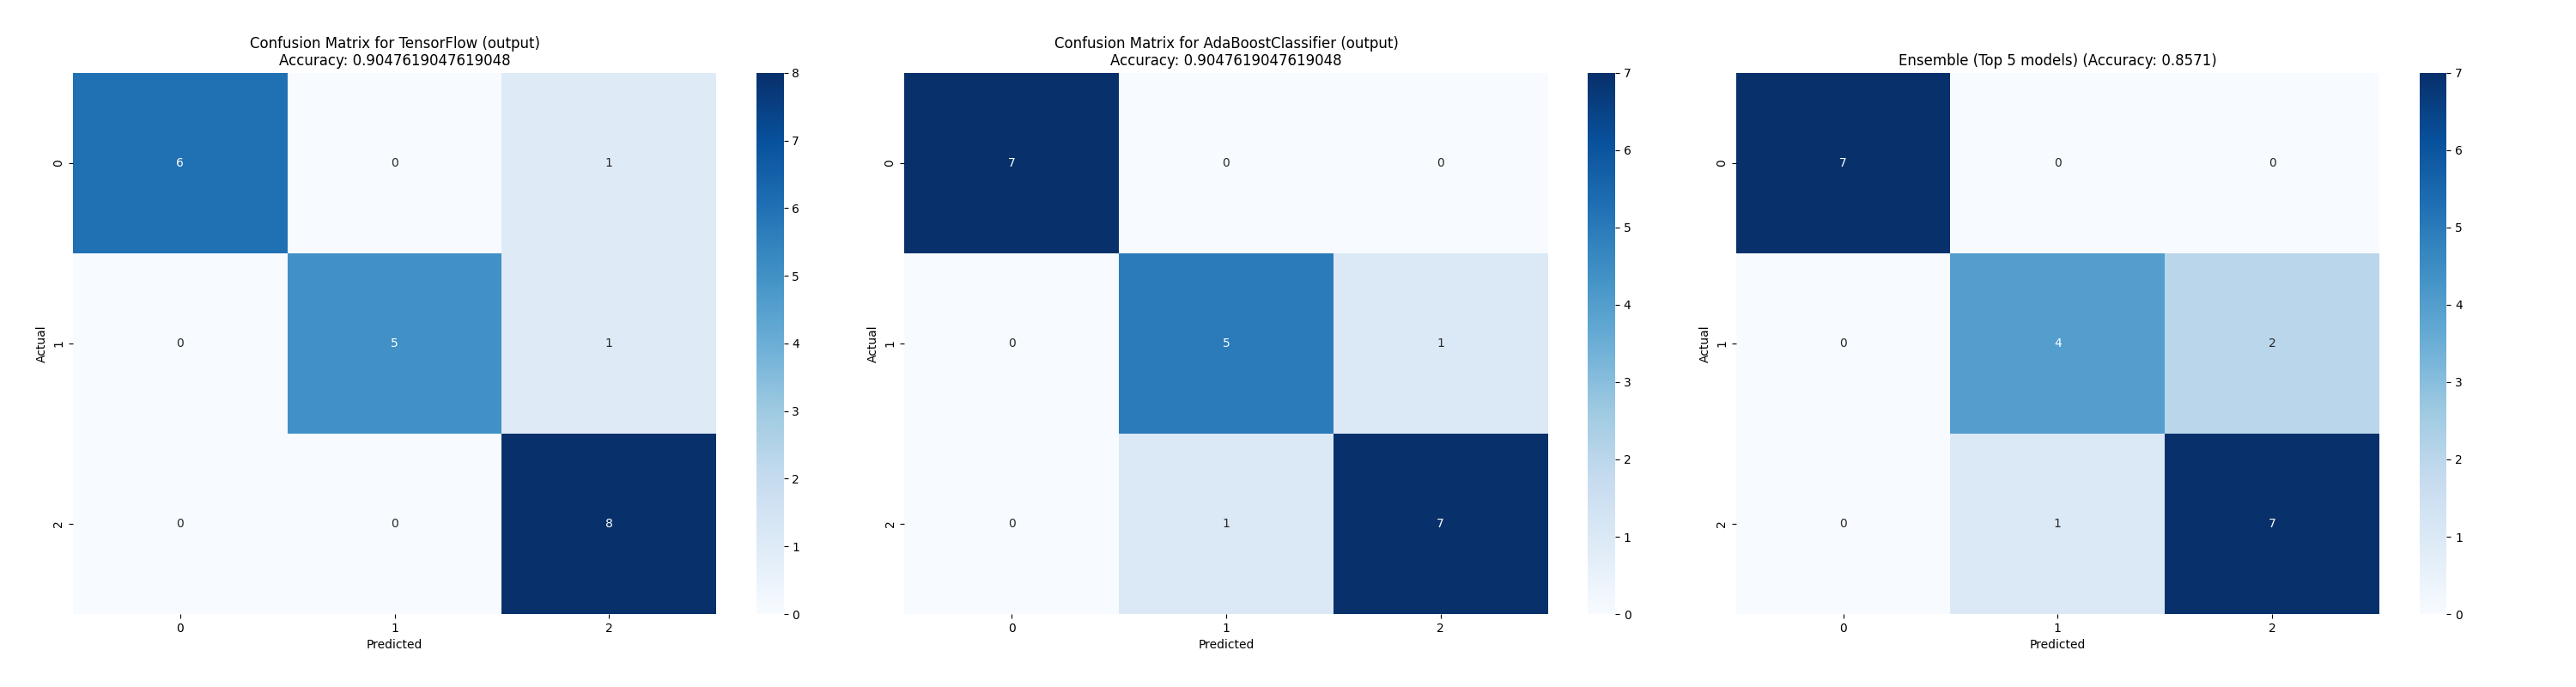
\includegraphics[width=0.95\linewidth]{class_all_section/top_2_and_ensemble_confusion_matrices_SFST_Benefit.png}
    \caption{Effect of EL on SFST Benefit using Classification and All Features}
    \label{fig_class_all:EL_SFST}
\end{figure}

This figure better demonstrate why ensemble learning can reduce the performance.
In this figure, the left most image represents the best model while the middle show the second best.
In the rightmost image we show the ensemble learning approach using the top five models.
Since the top models have few errors which differ from model to model, when combined the errors are more impactful.
This example demonstrates the negative side of ensemble learning.
Overall, these results demonstrate that \ac{ML} can be used to classify wetlands using the WESP-AC features.
Our next section delves into feature reduction techniques to reduce the input vector.


\subsubsection{Feature Reduction}\label{sec:class_all_featred}
Feature reduction consists of using techniques to reduce the input vector size.
In this section we explore the three feature reduction techniques, presented in section \ref{sec:PA}.

Using the accuracy as metric, we compare the algorithms for each \ac{EF} trained with reduced features.
The best performing algorithm for each function was selected based on accuracy from table \ref{tab_class_all:model_accuracies_best}.
Each algorithm was trained with the three reduction techniques with features ranging from two features all features.
We use graphical results and numerical results to analyze and compare our results.
In the annexe, figures \ref{fig_class_all:pr_featred_graph} to \ref{fig_class_all:sfst_ben_featred_graph} show the results for each \ac{EF} with the three reduction techniques.
In these figures, each \ac{EF} is showm with the accuracy for a varying number of features.
They provide us with better insight on the effect of the reducing the input features.
When looking closely such as figures \ref{class_all_tab:featred_sfst} and \ref{class_all_tab:featred_nr}, we better understand the results.
They respectively show the effect of feature reduction techniques for \ac{SR} Benefit and \ac{NR} Benefit.
In figure \ref{class_all_tab:featred_nr}, we can see how increasing the number of features has a proportionate effect on the accuracy.
It also shows the difference between the SelectKBest and \ac{VT} reduction techniques.
SelectKBest with the f classifier achieved maximum accuracy around 45 features while the other achieved it around 70 features.
\ac{VT} performed the worst and only achieved convergence using over 100 features.
We can see similar effects on \ac{SFST} Benefit when looking at figure \ref{class_all_tab:featred_nr}.

\begin{figure}[h]
    \centering
    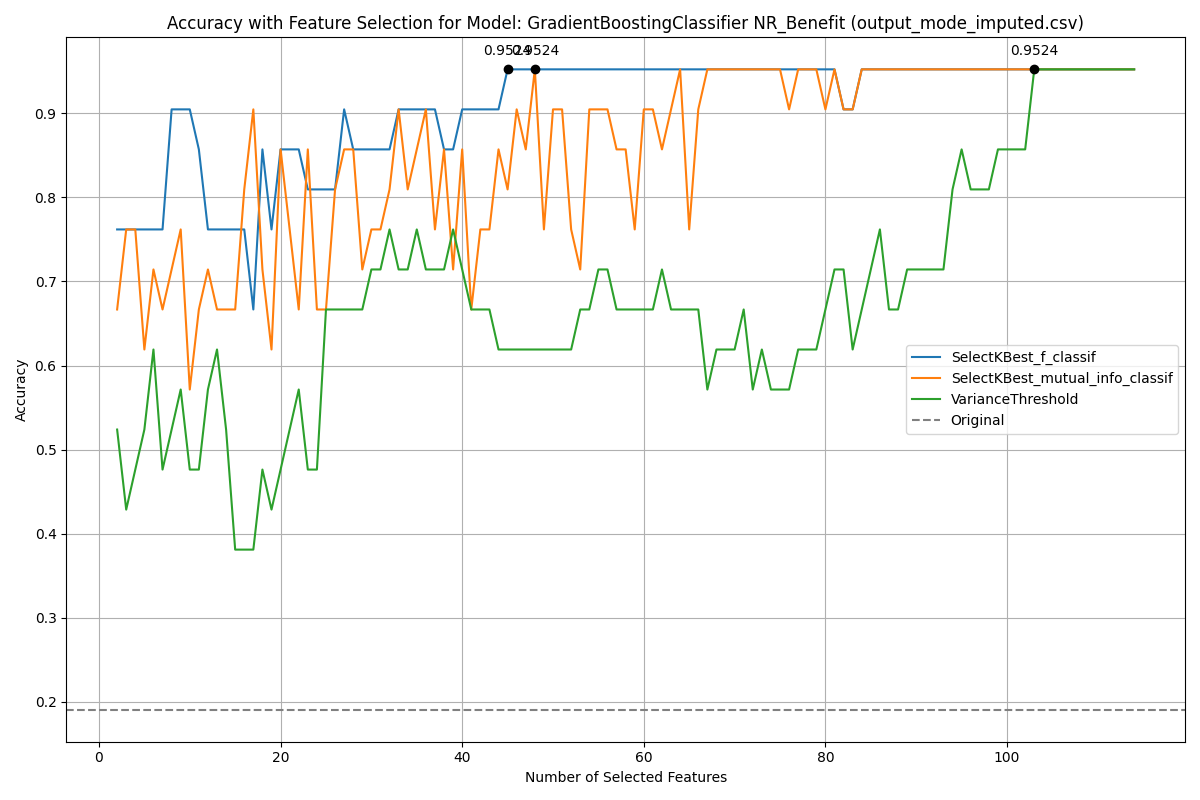
\includegraphics[width=0.85\linewidth]{class_all_section/feature_selection_accuracy_plot_output_mode_imputed.csv_GradientBoostingClassifier_NR_Benefit.png}
    \caption{NR Benefit Feature Reduction D4}
    \label{class_all_tab:featred_nr}
\end{figure}



\begin{figure}[h]
    \centering
    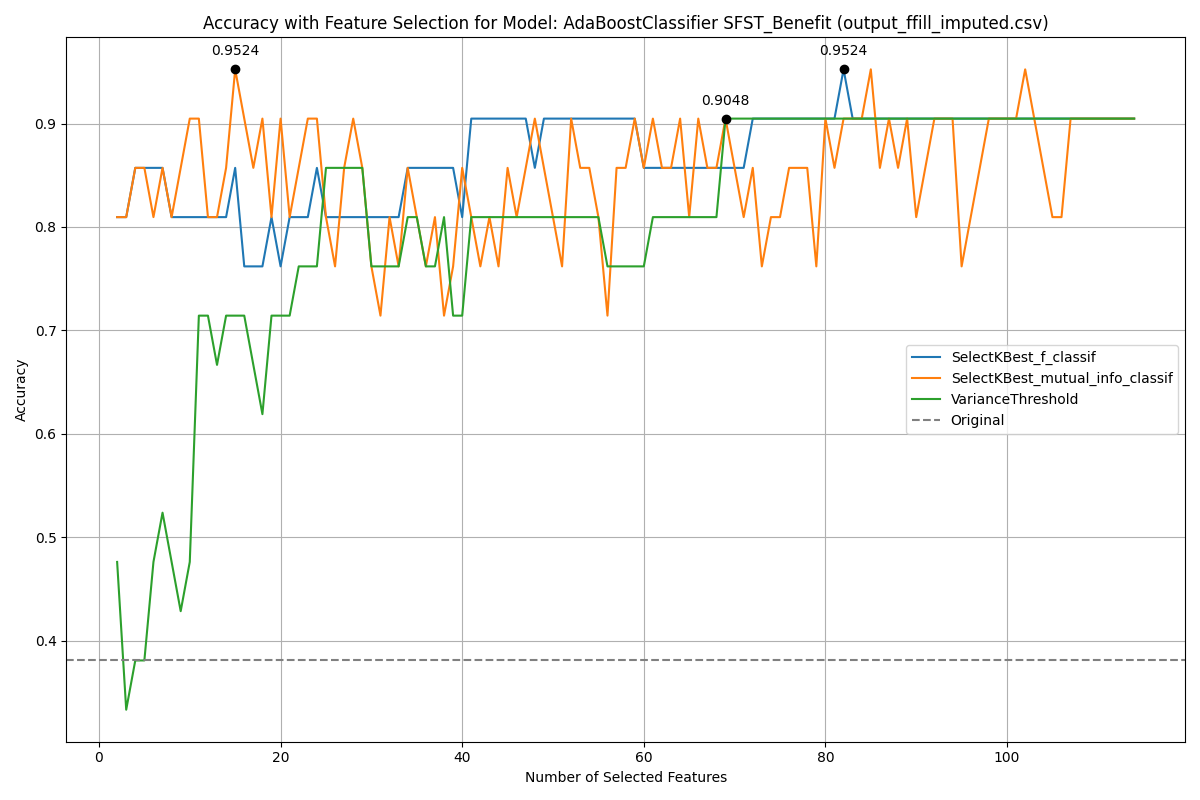
\includegraphics[width=0.85\linewidth]{class_all_section/feature_selection_accuracy_plot_output_ffill_imputed.csv_AdaBoostClassifier_SFST_Benefit.png}
    \caption{SFST Benefit Feature Reduction D4}
    \label{class_all_tab:featred_sfst}
\end{figure}

These results demonstrate that the SelectKBest technique significantly outperforms \ac{VT}.
It also shows how, using SelectKBest, the number of input features can be considerably reduced.
These hypothesis is further confirmed when looking at table \ref{tab_class_all:featred_small}.
This table shows the two best overall models that have considerably reduced features.
\begin{longtable}{|p{3cm}|p{3cm}|p{2cm}|p{2cm}|p{2cm}|}
\hline
\textbf{Function} & \textbf{Accuracy} &  \textbf{ Features} & \textbf{2nd Accuracy} &  \textbf{2nd Features}\\ \hline
\endfirsthead
\hline
\textbf{Function} & \textbf{Accuracy} &  \textbf{ Features} & \textbf{2nd Accuracy} &  \textbf{2nd Features}\\ \hline
\endhead

PR & 85.71\% & F43, F45 & 90.45\% &  F21, F23, F24, F28, F29, F31, F43, F44, F45 \\ \hline
NR & 80.85\% & F43, F44, F45 & 76.19\% &  F43, F44 \\ \hline
SR & 71.42\% & OF22, F35, F43, F45, F49 & 61.90\% & F43, F44 \\ \hline
WS & 85.71\% & F43, F44 & 85.71\% & F31, F43 \\ \hline
SFST & 95.24\% & F1, F43 & 95.24\% & F1, F24, F43 \\ \hline
PR Benefit & 85.71\% & OF22, F41 & 90.47\% & OF22, F41, F48, F50 \\ \hline
NR Benefit & 90.48\% & OF9, OF10, OF19, OF21, F41 & 80.95 \% & OF10, OF20, F41 \\ \hline
SR Benefit & 95.24\% & OF19, F41 & 100.0\% & OF19, OF21, F41\\ \hline
WS Benefit & 80.95\% & OF17, OF23 & 95.24\% & OF17, OF24, F51\\ \hline
SFST Benefit & 57.14\% & OF22, OF28 & 57.14\% & OF18, OF22, OF28 \\ \hline
\caption{Maximum Proportionate Accuracy}
\label{tab_class_spec:featred_small}
\end{longtable}

This table show our first interesting results for feature reduction of our \ac{ML} algorithms.
Using limited features, all of our \ac{EF}s achieved an accuracy anove 80\%.
In fact, all but three \ac{EF}s achieved an accuracy above 90\%.
\ac{SR}, \ac{NR} and \ac{PR} respectively achieved accuracies of 80.95\%, 80.95\% and 85.71\%.
When looking at our initial training results, both \ac{SR} and \ac{NR} achieved lower accuracies than other \ac{EF}s.
In fact, \ac{NR} achieved 80.95\% and \ac{SR} achieved 90.48\%.
These results explain why the accuracies are slightly lower than other \ac{EF}s during feature reduction.
However, even with lower results these models achieved impressive results.
Using only F43 and F44, we weer able to achieve accuracies of 80.95\% and 85.71\% for both \ac{NR} and \ac{PR}.
\ac{SR} required slightly more features and used F30, F31, F43, F44 and F45 to achieved an accuracy of 80.95\%.
\ac{WS} and \ac{SFST} performed very well and achieved respective accuracies of 90.45\% and 95.24\% using only two features.
\ac{WS} used F43 and F46 while \ac{SFST} used F43 and F44.
When looking at these results, a clear pattern can be seen in the choosen features.
The features F43 to F46 seem to play a major role in the ratings of wetlands.
F43 seems to be the most impactful with that feature appearing in all \ac{EF}s.

When looking at the Benefit ratings, the achieved accuracies are above the function ratings.
In fact, the accuracy range from 90.45\% to 100.00\% for the ratings.
However, they require slightly more features than the function scores.
An important note, the function ratings (e.g \ac{NR}, \ac{PR}) did not achieve higher scores with more features.
The accuracy was rarely higher than the results presented in table \ref{tab_class_all:featred_small}.
If rare case where accuracy was higher, the number of features used was considerably higher.
In terms of classifying the \ac{EF}s Benefit ratings, \ac{SR} Benefit achieved the best performance.
In fact, we achieved 100\% using four features (OF19, OF21, F21,F43) and 95.24\% using only OF19 and F41.
\ac{WS} Benefit also achieved good results with an accuracy of 95.24\% using only OF17 and OF23.
The results for \ac{WS} Benefit are exceptionally interesting due to our model using only OF features.
This would enable researchers to analyze the \ac{WS} \ac{EF} of wetlands without the need to ever go in the field.
\ac{NR} Benefit struggled to achieve good results with fewer features.
In fact, we only achieved an accuracy of 76.19\% when using three features (OF10, F43, F44).
When using eight features, we were able to achieved an accuracy of 90.45\%.
This \ac{EF} Benefit demonstrate that some may require considerably more features due to its complexity.
Similarly, \ac{PR} Benefit achieved 90.45\% using six features and 85.71\% using only F41 and F43.
Finally, \ac{SFST} Beneift achieved 90.45\% using 10 features and 80.95\% using both F43 and F44.
These results further demonstrate the difference between Function and Benefit ratings.
Both the Function and Benefit ratings achieved good performances using only a few features.
However, the Benefit ratings were able to be classified very well using four to eight features.
Overall when looking at the results, F41 to F46 seem to play a major role for both Function and Benefit ratings.
The Benefit ratings also seem to be more influenced by OF features than the Function ratings.
Both the Pronvicial and Federal classes seem to play a role in predicting certain \ac{EF}s.
This can be explained by the fact that those features could represent multiple features.


\paragraph{Ensemble Learning}
To increase the performance of our feature reduction approach, we propose implementing ensemble learning.
This is proposed to average out errors to increase the performance without retraining or the need for complex algorithms.
Our ensemble model, for each \ac{EF}, is based on the top five models achieved from the feature reduction with no more than 10 features per model.
Table \ref{tab_class_all:featred_ensemble} show the performance for each function before and after the ensemble learning.
\begin{longtable}{|p{2cm}|p{2cm}|p{2cm}|p{2cm}|p{4cm}|}
\hline
\textbf{Function} & \textbf{Best Acc.} & \textbf{2nd Best Acc.} & \textbf{Ensemble Learning Acc.} & \textbf{Features Used} \\ \hline
PR & 90.48\% & 85.71\% & 85.71\% & F1, F14, F28, F29, F43, F44, F45, FedClass, ProvClass \\ \hline
NR & 80.95\% & 80.95\% & 76.19\% & F43, F44, F45, F46 \\ \hline
SR & 80.95\% & 80.95\% & 80.95\% & F1, F14, F24, F28, F29, F30, F31, F3e, F41, F43, F44, F45, F46, FedClass, OF22, ProvClass \\ \hline
WS & 90.48\% & 90.48\% & 90.48\% & F43, F44, F45, F46 \\ \hline
SFST & 95.24\% & 95.24\% & 95.24\% & F43, F44, F45, F46 \\ \hline
PR Benefit & 90.48\% & 85.71\% & 85.71\% & F14, F24, F41, F43, F44, F46, F47 \\ \hline
NR Benefit & 90.48\% & 90.48\% & 85.71\% & F1, F14, F31, F3d, F41, F43, F44, F46, MossCover, OF10, OF19, OF9 \\ \hline
SR Benefit & 100.00\% & 100.00\% & 95.24\% & F14, F28, F29, F41, F43, F44, OF19, OF21 \\ \hline
WS Benefit & 95.24\% & 95.24\% & 95.24\% & F50, F52, F54, OF17, OF23, OF7 \\ \hline
SFST Benefit & 90.48\% & 85.71\% & 85.71\% & F1, F14, F23, F31, F43, F44, F45, F46, F5, Moss Cover, ProvClass \\ \hline
\caption{Ensemble Learning Accuracy}
\label{tab_class_all:featred_ensemble}
\end{longtable}


The top two models in this table are not necessarily the two models presented in table \ref{tab_class_all:featred_small}.
The five models choosen for ensemble learning were solely based on the highest accuracy with less than 10 features.
We choose using this approach rather than manually selecting models to remove any possible bias.
In this table, the first column represents the \ac{EF}, while the second and third represent the best and second best accuracy from section \ref{sec:class_all_featred}.
The fourth column represent the accuracy of the ensemble learning model while the last column consists of the features of all five models used for ensemble learning.
In this table, our earlier mention of ensemble learning reducing the accuracy is further confirmed.
In fact, seven out of ten \ac{EF}s were reduced by approximately 5\% while the others remain unchanged.
Furthermore, the number of features used was significantly increased.
However, ensemble learning could be beneficial if more training data was added.
Ensemble learning requires models to have datasets larger than our datasets.
Due to the smaller size of our dataset, our validation data was limited to 20 sites.
This means that a single error removes 5\% of the overall accuracy.
It also signifies that the ensemble learning approach can be significantly affected by a single missclassification.
For this reason ensemble learning does not benefit our algorithms as wanted.
Nonetless, without ensemble learning, our feature reduction techniques performed well.

\clearpage
\subsection{Specific Features}\label{sec:class_spec}
This section uses our D2 datasets which consists of only features specific to each \ac{EF}.
This considerably reduces the input vector from over 100 features to a range of six to 33.
Similar to the previous section, we compare our results using multiple data filling methods, however only the best is presented.
First, we present the training results and the ensemble learning approach using all D2 features in section \ref{sec:class_specific_results}.
Our ensemble learning algorithm consists of combining the top five best performing algorithms and average out the predictions.
Section \ref{sec:class_specific_featred} presents a feature reduction approach using the results from section \ref{sec:class_specific_results}.
In this section we compare the performance of our approach for \ac{EF} based on the prediction accuracy.
Our goal, as for the previous section, is to achieve good performance with minimum features.
We also explore ensemble learning on the reduced feature models.

\subsubsection{Training Results}\label{sec:class_specific_results}
We performed a grid search of our algorithms, hyperparameters data filling method of our D2 dataset.
Table \ref{tab_class_specific:model_accuracies_best} provides an overview of the best performing algorithms for each \ac{EF}.

\begin{table}[H]
\centering
\begin{tabular}{|c|c|p{4cm}|c|}
\hline
\textbf{Function} & \textbf{Model} & \textbf{Data} & \textbf{Accuracy} \\
\hline
PR & Ridge & All Data & 95.24\% \\
\hline
NR    & SGD. & Mean & 90.48\% \\
\hline
SR    & Tensorflow & Median & 100.00\% \\
\hline
WS    & GradientBoosting & All Data & 100.00\% \\
\hline
SFST  & GradientBoosting & All data & 95.24\% \\
\hline
PR Ben. & KNeighbors & All Data & 95.24\% \\
\hline
NR Ben. & SVC & All Data & 100.00\% \\
\hline
SR Ben.& Ridge, GradientBoosting & All Data & 100.0\% \\
\hline
WS Ben. & RandomForest & BFill, Custom, Interpolated, Iterative, Mean, Median, Mode & 95.24\% \\
\hline
SFST Ben. &  RandomForest & Custom, Mean & 71.42\% \\
\hline
\end{tabular}
\caption{Best Model Accuracies}
\label{tab_class_specific:model_accuracies_best}
\end{table}

In this table, each \ac{EF} is shown with the accuracy of the best performing model and data filling method.
A slight increase in performance can be observed when comparing these results with the results from using D4, found in table \ref{tab_class_all:model_accuracies_best}.
In fact, the accuracy has increased for five \ac{EF}s, remained unchanged for four and was reduced for one \ac{EF}.
Most impressively, using only specific features we achieved an accuracy of 100\% on five \ac{EF}.
Most impressively, \ac{SR} was increased from 90.48\% to 100.00\% and \ac{NR} from 80.95\% to 90.48\%.
However, \ac{SFST} Benefit was considerably reduced from 95.24\% in the previous section to 71.42\%.
We verified these results thoroughly and determined that a feature present in D4. but not D2, is important for this \ac{EF}.
Comparing the features for \ac{SFST} Benefit in table \ref{tab:data_spec_features} and the results from feature reduction using all features in table \ref{tab_class_all:featred_small}.
\ac{SFST} Benefit seems to mostly be based on OF questions while using all features demonstrated that F features are some of the most important.
Questions remain on why our models using specific features did not perform well for \ac{SFST} Benefit.
The data may be highly uncorrelated using specific features which could hinder the ability to learn.
Nonetheless, we achieved a very good performance on all other \ac{EF}s.


To increase the performance of our algorithms, we propose using ensemble learning to combine multiple models.
Overall, the ensemble learning did not increase the performance of our algorithms, as shown in table \ref{tab_class_specific:class_ensemble}.
\begin{table}[H]
\centering
\begin{tabular}{|c|c|c|}
\hline
\textbf{Function} & \textbf{Accuracy} & \textbf{Ensemble Accuracy} \\
\hline
PR      & 95.24\% & 95.24\% \\
\hline
NR      & 90.46\% & 85.71\%\\
\hline
SR      & 100.00\% & 100.00\%\\
\hline
WS      & 100.00\% & 100.00\%\\
\hline
SFST    & 95.24\% & 95.24\%\\
\hline
PR Ben. & 95.24\% & 100.00\%\\
\hline
NR Ben. & 100.00\% & 100.00\%\\
\hline
SR Ben. & 100.0\% & 100.0\%\\
\hline
WS Ben. & 95.24\% & 95.24\%\\
\hline
SFST Ben. & 71.42\% & 76.19\%\\
\hline
\end{tabular}
\caption{Ensemble Model Accuracies}
\label{tab_class_specific:class_ensemble}
\end{table}

\ac{SFST} Benefit was slightly improved from ensemble learning and was increased to 76.19\%, from 71.42\%.
Similarly, \ac{PR} Benefit was increased from 95.24\% to 100.00\%.

Figure \ref{fig_class_specific:EL_PR} and \ref{fig_class_specific:EL_SFST_ben} \ac{PR} Benefit and \ac{SFST} Benefit using the top two models and the ensemble learning using confusion matrices.

\begin{figure}
    \centering
    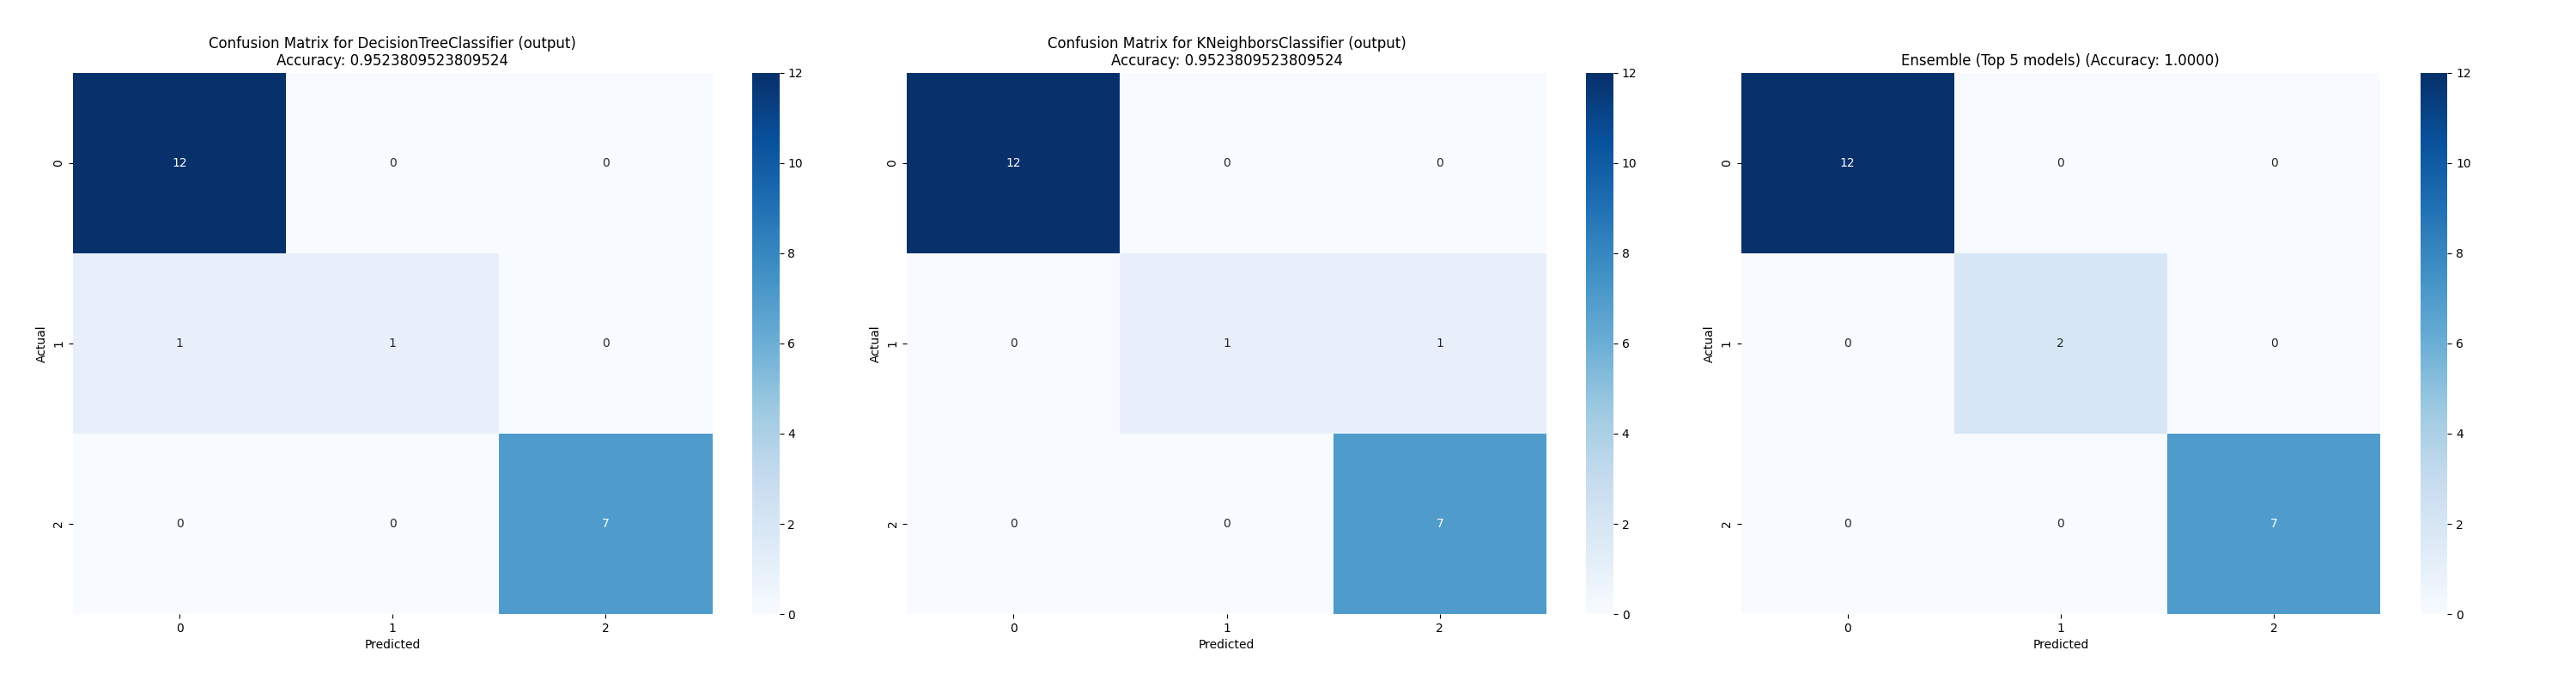
\includegraphics[width=0.95\linewidth]{class_specific_section/top_2_and_ensemble_confusion_matrices_PR_Benefit.png}
    \caption{Effect of EL on PR Benefit using Classification and Specific Features}
    \label{fig_class_specific:EL_PR}
\end{figure}

\begin{figure}
    \centering
    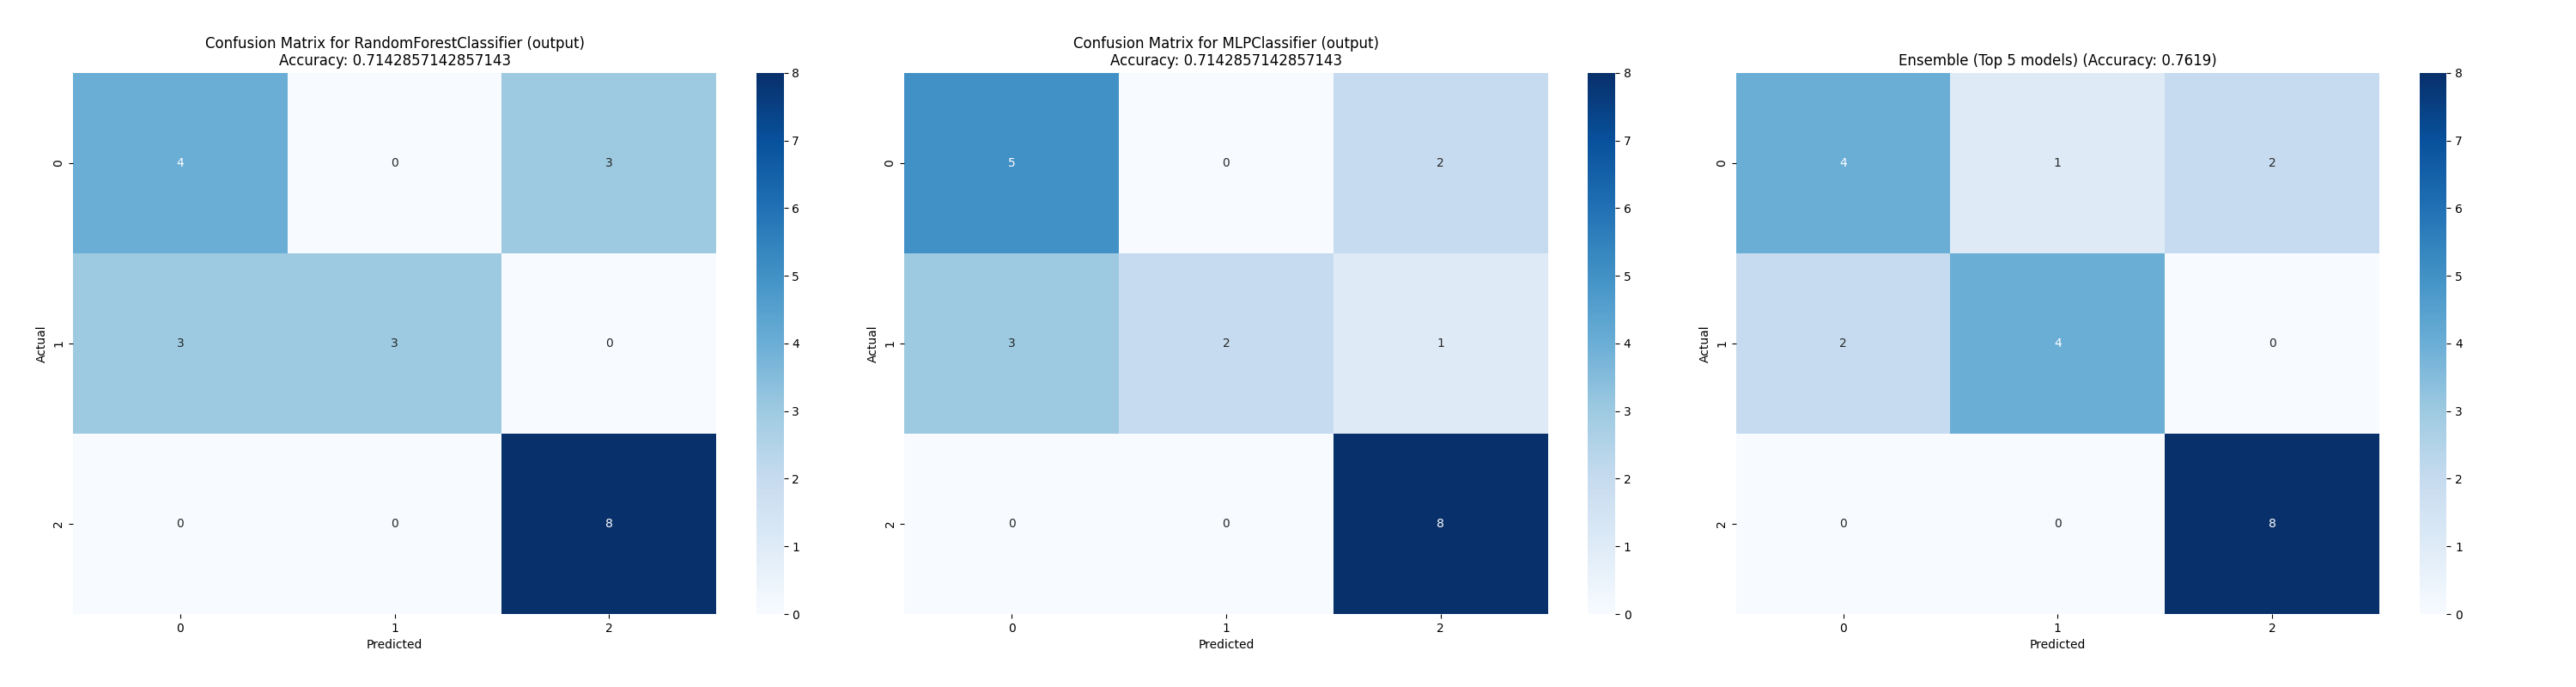
\includegraphics[width=0.95\linewidth]{class_specific_section/top_2_and_ensemble_confusion_matrices_SFST_Benefit.png}
    \caption{Effect of EL on SFST Benefit using Classification and Specific Features}
    \label{fig_class_specific:EL_SFST_ben}
\end{figure}

In these figures, we see how ensemble learning can increase the results by averaging missclassifications into their proper class.



\subsubsection{Feature Reduction}\label{sec:class_specific_featred}
As with D4, we use feature reduction techniques to reduce the input feature vector of our D2 dataset.
In this section we explore the three feature reduction techniques, presented earlier in section \ref{sec:PA}.
Using the accuracy as metric, we compare the algorithms for each \ac{EF} trained with reduced features.
The best performing algorithm for each function was selected based on the training accuracy from table \ref{tab_class_specific:model_accuracies_best}.
Each algorithm was trained with the three reduction techniques with features ranging from two to all features specific to the \ac{EF}.

Table \ref{tab_class_spec:featred_small} show the two best overall model for each \ac{EF} with reduced features.
\begin{longtable}{|p{3cm}|p{3cm}|p{2cm}|p{2cm}|p{2cm}|}
\hline
\textbf{Function} & \textbf{Accuracy} &  \textbf{ Features} & \textbf{2nd Accuracy} &  \textbf{2nd Features}\\ \hline
\endfirsthead
\hline
\textbf{Function} & \textbf{Accuracy} &  \textbf{ Features} & \textbf{2nd Accuracy} &  \textbf{2nd Features}\\ \hline
\endhead

PR & 85.71\% & F43, F45 & 90.45\% &  F21, F23, F24, F28, F29, F31, F43, F44, F45 \\ \hline
NR & 80.85\% & F43, F44, F45 & 76.19\% &  F43, F44 \\ \hline
SR & 71.42\% & OF22, F35, F43, F45, F49 & 61.90\% & F43, F44 \\ \hline
WS & 85.71\% & F43, F44 & 85.71\% & F31, F43 \\ \hline
SFST & 95.24\% & F1, F43 & 95.24\% & F1, F24, F43 \\ \hline
PR Benefit & 85.71\% & OF22, F41 & 90.47\% & OF22, F41, F48, F50 \\ \hline
NR Benefit & 90.48\% & OF9, OF10, OF19, OF21, F41 & 80.95 \% & OF10, OF20, F41 \\ \hline
SR Benefit & 95.24\% & OF19, F41 & 100.0\% & OF19, OF21, F41\\ \hline
WS Benefit & 80.95\% & OF17, OF23 & 95.24\% & OF17, OF24, F51\\ \hline
SFST Benefit & 57.14\% & OF22, OF28 & 57.14\% & OF18, OF22, OF28 \\ \hline
\caption{Maximum Proportionate Accuracy}
\label{tab_class_spec:featred_small}
\end{longtable}

At first glance, this dataset unperformed D4 with this dataset achieving accuracies ranging from 71.42\% to 95.24\%. 
using D2, all \ac{EF}s achieved lower accuracies than the reduced features using the D4 dataset.
\ac{SFST} Benefit was the most affected with its accuracy reduced from 80.95\% using two features to 57.14\%.
Overall, it seem that using all available features and then reducing them using algorithms achieve better results than using specific features.
This could be explained by the fact that certain features, that are not found in D2, combine the uniqueness of specific features.


In the annex, figures \ref{fig_class_spec:pr_featred_graph} to \ref{fig_class_spec:sfst_ben_featred_graph} who the effect of the various feature reduction techniques.
Figure \ref{class_spec_tab:featred_pr} below show the effect of feature reduction techniques for \ac{WS}.

\begin{figure}
    \centering
    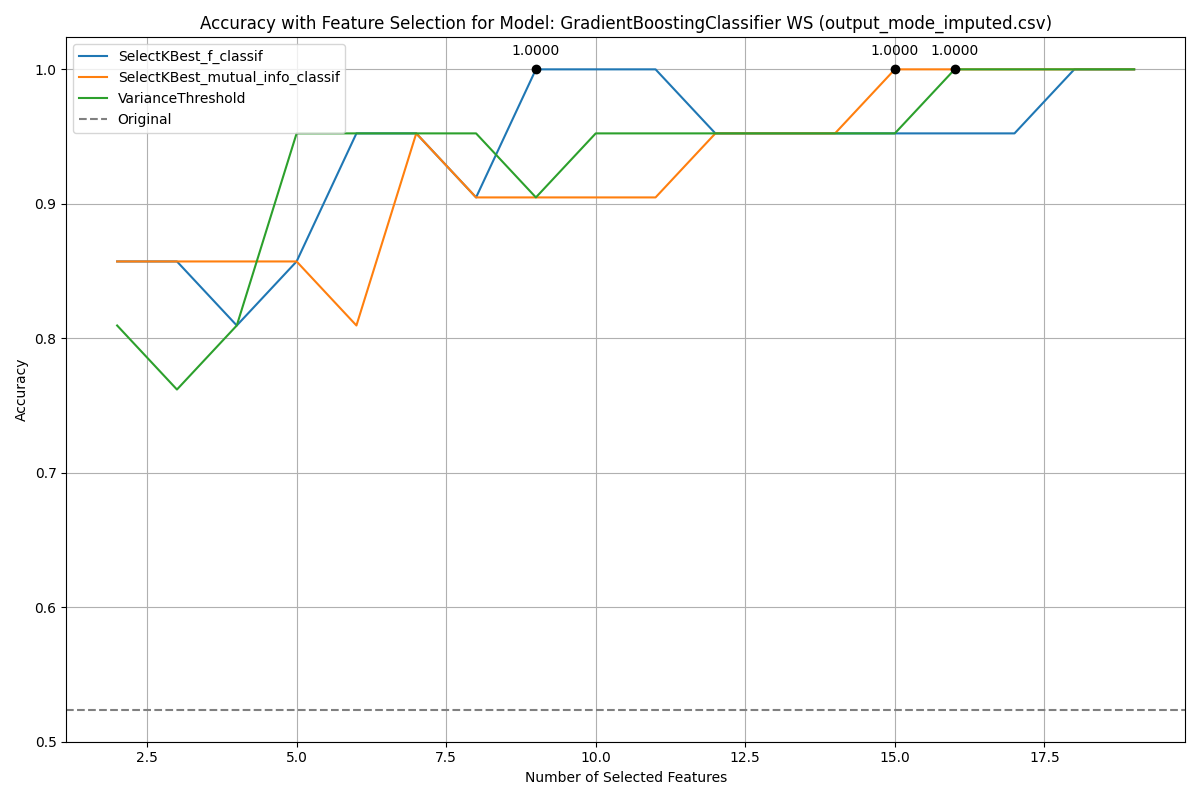
\includegraphics[width=0.85\linewidth]{class_specific_section//images_class_ensemble_reduction/feature_selection_accuracy_plot_output_mode_imputed.csv_GradientBoostingClassifier_WS.png}
    \caption{WS Feature Reduction D4}
    \label{class_spec_tab:featred_pr}
\end{figure}


In this figure, the difference mentioned earlier between \ac{SKB} and \ac{VT} can be seen again.
\ac{SKB} outperformed \ac{VT} significantly and converged more quickly and efficiently.
In fact, \ac{SKB} with F classifier achieved 100.00\% accuracy using nine features while \ac{VT} required 15.
This figure demonstrates the importance of analyzing our results to better understand its behavior.



\paragraph{Ensemble Learning}
To increase the performance of our feature reduction approach, we propose using ensemble learning.
This is proposed to average out errors to increase the performance without retraining or the need for complex algorithms.
Our ensemble model, for each \ac{EF}, is based on the top five models achieved from the feature reduction with no more than 10 features per model.
Table \ref{tab_class_spec:featred_ensemble} show the performance for each function before and after the ensemble learning.

\begin{longtable}{|p{2cm}|p{2cm}|p{2cm}|p{2cm}|p{4cm}|}
\hline
\textbf{Function} & \textbf{Best Acc.} & \textbf{2nd Best Acc.} & \textbf{Ensemble Learning Acc.} & \textbf{Features Used} \\ \hline
PR & 90.48\% & 85.71\% & 85.71\% & F1, F14, F28, F29, F43, F44, F45, FedClass, ProvClass \\ \hline
NR & 80.95\% & 80.95\% & 76.19\% & F43, F44, F45, F46 \\ \hline
SR & 80.95\% & 80.95\% & 80.95\% & F1, F14, F24, F28, F29, F30, F31, F3e, F41, F43, F44, F45, F46, FedClass, OF22, ProvClass \\ \hline
WS & 90.48\% & 90.48\% & 90.48\% & F43, F44, F45, F46 \\ \hline
SFST & 95.24\% & 95.24\% & 95.24\% & F43, F44, F45, F46 \\ \hline
PR Benefit & 90.48\% & 85.71\% & 85.71\% & F14, F24, F41, F43, F44, F46, F47 \\ \hline
NR Benefit & 90.48\% & 90.48\% & 85.71\% & F1, F14, F31, F3d, F41, F43, F44, F46, MossCover, OF10, OF19, OF9 \\ \hline
SR Benefit & 100.00\% & 100.00\% & 95.24\% & F14, F28, F29, F41, F43, F44, OF19, OF21 \\ \hline
WS Benefit & 95.24\% & 95.24\% & 95.24\% & F50, F52, F54, OF17, OF23, OF7 \\ \hline
SFST Benefit & 90.48\% & 85.71\% & 85.71\% & F1, F14, F23, F31, F43, F44, F45, F46, F5, Moss Cover, ProvClass \\ \hline
\caption{Ensemble Learning Accuracy}
\label{tab_class_all:featred_ensemble}
\end{longtable}


In this table, the first column represents the \ac{EF}, while the second and third represent the best and second best accuracy from section \ref{sec:class_specific_featred} with a maximum of 10 features.
The fourth column represent the accuracy of the ensemble learning model while the last column consists of the features of all five models used for ensemble learning.
As per the previous sections, ensemble learning did not increase the performance of our models.





\subsection{Dataset Comparaison}
To more easily compare the difference in results, we present the best performing models for each \ac{EF} for both classification and regression.
We present the models which achieved the most interesting results in table \ref{tab_combined:featred_accuracy}.

\begin{longtable}{|p{3cm}|p{2cm}|p{3cm}|p{2cm}|p{3cm}|}
\hline
\textbf{Function} & \textbf{Acc. All} & \textbf{Features All} & \textbf{Acc. Specific} & \textbf{Features Specific} \\ \hline
\endfirsthead
\hline
\textbf{Function} & \textbf{Acc. All} & \textbf{Features All} & \textbf{Acc. Specific} & \textbf{Features Specific} \\ \hline
\endhead

PR & 85.71\% & F43, F45 & 85.71\% & F43, F45 \\ \hline
NR & 80.95\% & F43, F44 & 80.85\% & F43, F44, F45 \\ \hline
SR & 80.95\% & Hydrogeo., F24, F29, F43, F44, F45 & 71.42\% & OF22, F35, F43, F45, F49 \\ \hline
WS & 90.45\% & F43, F46 & 85.71\% & F43, F44 \\ \hline
SFST & 95.24\% & F43, F44 & 95.24\% & F1, F43 \\ \hline
PR Benefit & 90.45\% & F14, F24, F41, F43, F46, F47 & 85.71\% & OF22, F41 \\ \hline
NR Benefit & 90.45\% & MossCover, OF9, OF10, OF19, F1, F14, F41, F43 & 90.48\% & OF9, OF10, OF19, OF21, F41 \\ \hline
SR Benefit & 100.00\% & OF19, OF21, F41, F43 & 95.24\% & OF19, F41 \\ \hline
WS Benefit & 95.24\% & OF17, OF23 & 80.95\% & OF17, OF23 \\ \hline
SFST Benefit & 90.45\% & ProvClass, MossCover, F1, F5, F23, F31, F43, F44, F45, F46 & 57.14\% & OF22, OF28 \\ \hline
\caption{Comparison of Best Accuracy and Features from Two Tables}
\label{tab_combined:featred_accuracy}
\end{longtable}

In this table, the first column presents the \ac{EF} while the second and fourth present the accuracy for the D4 and D2 datasets respectively.
Similarly, column three and five show the respective features for the second and fourth columns.
Overall, classification using all features performed better than using specific features.
In fact, all \ac{EF} achieved a better classification using all features.
We also demonstrated that we were able to classify the ratings of \ac{EF} for wetlands using limited features.
Some \ac{EF}s, such as \ac{WS} Benefit achieved an accuracy of 95.24\% using only two features.
These exploratory results are highly impressive and further improve them would be interesting.
Adding more sites to our datasets would be the most beneficial improvement.
Due to the limited amount of wetlands, our models are not guaranteed to perform well to new parameters.
Our models could struggle significantly on wetlands which are abnormal compared to training data.
Wetlands from other provinces or from unique regions in the same province could cause issues.
We recommend using our results as exploratory and not definitive.
Our results should be used only to demonstrate the possibilities of using classification and feature reduction techniques.
Using larger validation samples and test samples would be required in next iterations of in this work.


\clearpage


\section{Regression}\label{sec:regression}
Regression is a common type of algorithm used in \ac{ML} with a key difference from classification.
Classification predicts a class, such as 0 or 1, while regression predicts a continuous value.
In our case, the continuous value would be the score for the function or benefit of an \ac{EF}.
The classification results from \ref{sec:class} have shown great promise and is interesting for the project.
However, the algorithms trained for classification used the normalized scores, for both the function and benefit.
In turn, the algorithms are specific to regions, such as for NB, and depend on the calibration wetlands.
If different calibration wetlands are used or the region modified, the algorithms could underperform significantly.
For this reason, we propose using regression to predict the non-normalized and normalized scores of the various \ac{EF}.
We propose using the non-normalize score such that it does our approach does not depend on calibration sites or region.
However, we also compare using pre-normalized scores to compare the results.
The data was collected, modified and generated using simple pre-processing techniques as seen from section \ref{sec:data}.
We present our results using both D4 and D2 datasets, respectively using all features and specific features.
We use the Mean Squared Error (MSE) as metric, which averages the squares of the errors and is defined in equation \ref{eq:mse}.
\begin{equation}
\text{MSE} = \frac{1}{n} \sum_{i=1}^n (y_i - \hat{y}_i)^2
\label{eq:mse}
\end{equation}

\subsection{All Features}
Similar to our classification technique, we perform a grid search of various regression algorithms, hyperparamters and data filling methods.
We trained our algorithms and techniques for \ac{PR}, \ac{NR}, \ac{SR}, \ac{WS} and \ac{SFST}, for both the Function and Benefit.
More information about the training procedure can be found within the GITHUB, under regression.
The algorithms used for regression are shown in table \ref{tab:all_algorithms}.
Similar to classification, we first propose comparing the regression algorithms using all features for the \ac{EF}.
We compare our training results, feature reduction techniques and class grouping.
Class grouping consists of classifying the regression predictions such that we can compare our regression and classification.
We perform the same tests using our D2 datasets which consists of specific features only.

\subsubsection{Training Results}
First we show the training results using the top accuracy over any algorithm and data filling method in table \ref{reg_all_tab:mse_summary}.
This table shows the MSE for the non-normalized (NNorm), normalized (Norm) and pre-normalized (PNorm) predictions of the best models.
Using this figure, we can see a significantly increase in MSE when comparing NNorm and Norm.
In fact, the MSE is often doubled when normalizing the prediction from using NNorm.
This is expected since normalizing predictions scales the errors into a bigger scale.
When comparing NNorm and PNorm, NNorm achieved better results when comparing \ac{EF} Functions.
When looking at \ac{EF} Benefits, NNorm performed better on \ac{PR} and \ac{WS} while PNorm performed better on \ac{SR}, \ac{NR} and \ac{WS}. 
NNorm achieved an MSE of 1.19 for \ac{WS} Benefit while PNorm achieved a lower MSE of 0.63.
On the contrary, PNorm achieved an MSE of 0.49 for \ac{PR} Benefit while NNorm achieved 0.22.
This difference in results demonstrate the purpose of comparing both NNorm and PNorm data. 

\begin{table}[H]
\centering
\begin{tabular}{|c|c|c|c|}
\hline
\textbf{Feature} & \textbf{Non-Normalized MSE} & \textbf{Normalized MSE} & \textbf{Pre-Normalized MSE} \\
\hline
NR & 0.17 & 0.48 & 0.31 \\
\hline
PR & 0.12 & 0.19 & 0.21 \\
\hline
SR & 0.37 & 0.62 & 0.46 \\
\hline
SFST & 0.20 & 0.33 & 0.26 \\
\hline
WS & 0.25 & 0.49 & 0.60 \\
\hline
NR Benefit & 0.39 & 0.45 & 0.28 \\
\hline
PR Benefit & 0.22 & 0.23 & 0.49 \\
\hline
SR Benefit & 0.17 & 0.22 & 0.07 \\
\hline
SFST Benefit & 0.51 & 0.98 & 0.71 \\
\hline
WS Benefit & 1.19 & 1.21 & 0.63 \\
\hline
\end{tabular}
\caption{Summary of Best MSE for Non-Normalized, Normalized, and Pre-Normalized Data}
\label{reg_all_tab:mse_summary}
\end{table}


In the annex, tables \ref{reg_all_tab:norm_mse} and \ref{reg_all_tab:pre_norm_mse} respectively show the full results for the NNorm, Norm and PNorm data.
In terms of algorithm, the AdaBoost regressor has achieved an overall better performance.
The MLP and SGD regressor were also found to be effective at predicting the scores.
In terms of data filling method, each \ac{EF} had their best one but overall each performed similarly.
The results presented in this section demonstrated interesting results.
It showed that both NNorm and PNorm data can be used for regression while Norm should not be prioritized.


We also implemented ensemble learning in the goal to increase our performance.
Table \ref{reg_all_tab:ensemble} presents the results with and without ensemble learning for all three normalization.
In this table, we can see that our results were not significantly impacted by ensemble learning.
The MSE for \ac{NR} Benefit using NNorm was slightly reduced from 0.39 to 0.27 while \ac{WS} Benefit was reduced to 0.86 from 1.19.
This small increase in performance could be beneficial for our class grouping.


\begin{table}[H]
\centering
\begin{tabular}{|c||c|c|c||c|c|c|}
\hline
\multirow{2}{*}{\textbf{Feature}} & \multicolumn{3}{c||}{\textbf{Training}} & \multicolumn{3}{c|}{\textbf{Ensemble Learning}} \\
\cline{2-7}
 & \textbf{Non-Norm} & \textbf{Norm} & \textbf{Pre-Norm} & \textbf{Non-Norm} & \textbf{Norm} & \textbf{Pre-Norm} \\
\hline
PR & 0.12 & 0.19 & 0.21 & 0.12 & 0.19 & 0.22 \\
\hline
NR & 0.17 & 0.48 & 0.31 & 0.17 & 0.48 & 0.28 \\
\hline
SR & 0.37 & 0.62 & 0.46 & 0.39 & 0.65 & 0.50\\
\hline
WS & 0.25 & 0.49 & 0.60 & 0.25 & 0.49 & 0.61 \\
\hline
SFST & 0.20 & 0.33 & 0.26 & 0.21 & 0.36 & 0.27\\
\hline
NR Benefit & 0.39 & 0.45 & 0.28 & 0.27 & 0.64 & 0.36 \\
\hline
PR Benefit & 0.22 & 0.23 & 0.49 & 0.31 & 0.32 & 0.31 \\
\hline
SR Benefit & 0.17 & 0.22 & 0.07 & 0.13 & 0.17 & 0.06 \\
\hline
WS Benefit & 1.19 & 1.21 & 0.63 & 0.86 & 0.87 & 0.68 \\
\hline
SFST Benefit & 0.51 & 0.98 & 0.71 & 0.38 & 0.72 & 0.60 \\
\hline
\end{tabular}
\caption{Ensemble Learning Effect on All Features Training}
\label{reg_all_tab:ensemble}
\end{table}

In the annexe, figures \ref{reg_all_fig:pr_ensemble} to \ref{reg_all_fig:sfst_ben_ensemble} show graphs with the algorithms and ensemble learning.
In these figures, we present all three normalization techniques with each their top three models and their ensemble approach.
When looking at the overall clusters of normalization for each \ac{EF}, we can observe the difference between normalized and non-normalized data.
Normalized data, either post or pre-normalized, were more spread out while non-normalized data was often in small clusters.
This demonstrates the benefit of using normalized data since it provides a more usable range.
However, it also showcases the issue with using pre-normalized data.
Whern using pre-normalized data, our model is bounded by the normalization unless the model is retrained.
Using our models to predict non-normalize scores while normalizing the predictions offers the benefits without the issues.

When looking at the \ac{WS} Benefit figure \ref{reg_all_fig:ws_ben_ensemble}, it demonstrates the powerfullness of ensemble learning.
More specifically, looking at the NNorm results we can observe that one model always over estimates while two underestimate.
However, with the ensemble learning these results are averaged out and a better prediction is achieved.
These figures, such as figure \ref{reg_all_fig:sfst_ensemble}, demonstrates how well our models performed.
In fact, in this figure most sites were predicted correctly with only one missclassification.
However, this figure demonstrates how well our models were able to group clusters.



Table \ref{reg_all_tab:summary_class_grouping} show the class grouping while tables \ref{reg_all_tab:grouping_non_norm_accuracy}, \ref{reg_all_tab:grouping_norm_accuracy} and \ref{reg_all_tab:grouping_pre_norm_accuracy} show the detailed results in the annex.


\begin{table}[H]
\centering
\begin{tabular}{|c||c|c||c|c||c|c|}
\hline
\multirow{2}{*}{\textbf{Feature}} & \multicolumn{2}{c||}{\textbf{Non-Norm}} & \multicolumn{2}{c||}{\textbf{Norm}} & \multicolumn{2}{c|}{\textbf{Pre-Norm}} \\
\cline{2-7}
 & \textbf{Overall} & \textbf{Ensemble} & \textbf{Overall} & \textbf{Ensemble} & \textbf{Overall} & \textbf{Ensemble} \\
\hline
PR & 100.00\% & 95.24\% & 90.48\% & 90.48\% & 100.00\% & 95.24\% \\
\hline
NR & 90.48\% & 90.48\% & 85.71\% & 85.71\% & 85.71\% & 85.71\% \\
\hline
SR & 100.00\% & 100.00\% & 100.00\% & 95.24\% & 100.00\% & 100.00\%\\
\hline
WS & 100.00\% & 100.00\% & 100.00\% & 95.24\% & 100.00\% & 100.00\% \\
\hline
SFST & 85.71\% & 85.71\% & 100.00\% & 95.24\% & 100.00\% & 95.24\% \\
\hline
PR\_Benefit & 90.48\% & 90.48\% & 95.24\% & 90.48\% & 90.48\% & 90.48\% \\
\hline
NR\_Benefit & 95.24\% & 95.24\% & 100.00\% & 95.24\% & 100.00\% & 100.00\% \\
\hline
SR\_Benefit & 95.24\% & 95.24\% & 95.24\% & 95.24\% & 95.24\% & 95.24\% \\
\hline
WS\_Benefit & 100.00\% & 100.00\% & 100.00\% & 100.00\% & 100.00\% & 100.00\% \\
\hline
SFST\_Benefit & 90.48\% & 90.48\% & 95.24\% & 90.48\% & 95.24\% & 95.24\% \\
\hline
\end{tabular}
\caption{Summary of Overall and Ensemble Accuracy for Non-Normalized, Normalized, and Pre-Normalized Data}
\label{reg_all_tab:summary_class_grouping}
\end{table}

In table \ref{reg_all_tab:summary_class_grouping}, we present the class grouping accuracies for all three normalization.
For non-normalized, values were not normalized but the same boundaries for the classes were used as the normalized data.
All three methods achieved similar results with Norm and PNorm achieving slightly better results on most \ac{EF}s.
However, NNorm performed better on \ac{NR} than either normalized data and achieved 90.48\% compared to 85.71\% for normalized.
Over all three normalization techiques, we achieved six 100\%, three 95.24\% and one 90.48\%.
These results are highly promising and demonstrated that regression can be used for predicting the scores.
Not only can they accurately predict the scores, they are able to use those scores to classify the sites.
When compared against our classification models, our regression models significantly outperforms them.
In fact, using all features we achieved an average accuracy of 93.811\% for classification and 97.62\% for regression.  
This difference is important especially with the possibility of using regression to directly predict the scores. 
Similar to classification, \ac{NR} had difficulties converging to a good model compared to the other \ac{EF}s.
Further exploration into this would be highly beneficial in next iterations of this project.

\subsubsection{Feature Reduction}
Similar to classification, our primary goal is to achieve similar results with considerably less features.
Table \ref{reg_all_tab:featred_res} show our most promising results.

\begin{table}[H]
\centering
\begin{tabular}{|c|c|c|p{4cm}|c|p{4cm}|}
\hline
\textbf{Function} & \textbf{NNorm} & \textbf{Norm} & \textbf{Features} & \textbf{PNorm} & \textbf{Features} \\
\hline
PR & 0.3721 & 0.5917 & F43, F44, F45 & 0.5237 & F43, F44, F45, Federal\_Class \\
\hline
SR & 0.6319 & 1.0629 & F24, F28, F29, F31, F43 & 0.8303 & F24, F28, F29, F44 \\
\hline
NR & 0.2786 & 0.5506 & F24, F43, F44, F45 & 0.7361 & F24, F43, F44, F45 \\
\hline
WS & 0.2627 & 0.5250 & F22, F24, F31, F43 & 0.4642 & F22, F31, F43 \\
\hline
SFST & 0.2953 & 0.4967 & F30, F43, F44, F45, F46 & 0.5688 & F43, F44\\
\hline
\hline
PR\_Benefit & 1.2611 & 1.3809 & F14, F41, F43, OF19 & 1.3627 & F14, F41, F43, OF19 \\
\hline
SR\_Benefit & 0.6983 & 0.6315 & F41, OF19, OF20, OF21 & 2.0620 & F41, OF19, OF21 \\
\hline
NR\_Benefit & 3.0280 & 3.5086 & F14, F41, OF10, OF19, OF9 & 3.4702 & F14, OF10, OF19, OF9 \\
\hline
WS\_Benefit & 0.7507 & 0.7629 & F51, F65, OF17, OF23, OF24 & 0.9022 &  Hydrogeo., OF17, OF23, OF24 \\
\hline
SFST\_Benefit & 1.1648 & 2.2533 & F1, F43, F44, F46 & 2.3641 & F43, F44 \\
\hline
\end{tabular}
\caption{Best MSE with Corresponding Features}
\label{reg_all_tab:featred_res}
\end{table}


In this table, we present each function with the best NNorm and PNorm models.
We choose the models for each based on the lowest MSE with a maximum of five features.
We present both their MSE and features used with the addition of the MSE for the normalized values of NNorm, named Norm.
Overall, Norm achieved a higher MSE than NNorm with certain \ac{EF} more than quadrupling their MSE.
Certain \ac{EF}s achieved a lower MSE when normalizing the NNorm data.
\ac{SR} Benefit had its MSE reduced from 0.6983 to 0.6315 using the same NNorm model but normalizing the predictions.
It even achieved a lower MSE than by using the PNorm dataset.
NNorm obtained the overall best MSE which could be caused by the range of values being lower.
By using a smaller range, the models can easily learn to predict the values into a smaller cluster, thus reducing the MSE.
Using NNorm data could easily provide a solution to pinpoint the exact score.
However, since our goal is to classify these sites into our three classes, we must normalize them accordingly.
In terms of normalization, PNorm has a clear advatange over the Norm data.
It achieved a better MSE on most \ac{EF} and, more importantly, was consistent across all \ac{EF}s.
In this table, we can also observe a reccuring issue with \ac{NR} Benefit not converging with either NNorm, Norm or PNorm.
In fact, compared to other \ac{EF} functions using NNorm, it achieved 3.0280 compared to the second highest at 0.2.2611.
For PNorm, \ac{NR} achieved an MSE of 3.4702 compared to the second highest at 2.3641.
Further exploration into this issue would benefit our project in future iterations.
Other than \ac{NR} Benefit, other \ac{EF}s achieved good scores using either NNorm and PNorm.
Similar to classifcation, the \ac{EF} Functions converged more efficiently than the Benefits.
In terms of input features, the WESP-AC features are mostly used with the exception of the hydrogeomorphic class in \ac{PR} Benefit for PNorm.
These results demonstrate that using the extra data may not be viable solution.
More information can be found in the supplementary data which has a section dedicated on using only extra features.
This experiment further confirmed our suspicion that the extra features were not beneficial currently.
Adding more wetland sites or different extra features could possible yield interesting results.


In terms of reduction technique, both \ac{SKB} significantly outperformed \ac{VT} for all \ac{EF}s.
Figure \ref{reg_all_fig:featred_Ex} show the effect of the various feature reduction techniques on \ac{WS}.

\begin{figure}
    \centering
    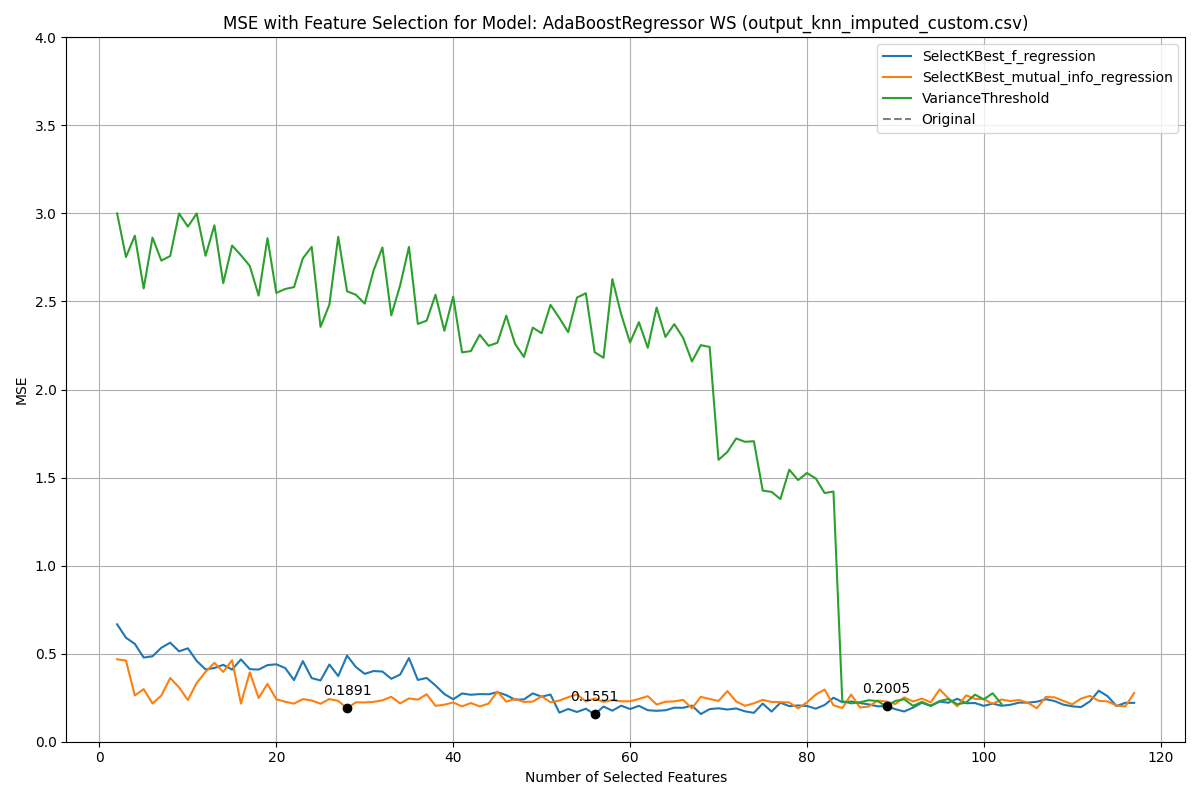
\includegraphics[width=1\linewidth]{reg_section_all/feature_selection_WS_non_norm.png}
    \caption{WS Non-Norm Feature Reduction}
    \label{reg_all_fig:featred_Ex}
\end{figure}
In this figure, we can observe that both \ac{SKB} quickly found the most important features while \ac{VT} did not.
This pattern is repeated for all \ac{EFs} using any NNorm, Norm or PNorm.



Using the top five models, Table \ref{reg_all_tab:summary_mse_features} show our models with ensemble learning.

\begin{table}
\centering
\begin{tabular}{|c||c|p{2.5cm}||c|p{2.5cm}||c|p{2.5cm}|}
\hline
\multirow{2}{*}{\textbf{Feature}} & \multicolumn{2}{c||}{\textbf{NNorm}} & \multicolumn{2}{c||}{\textbf{Norm}} & \multicolumn{2}{c|}{\textbf{PNorm}} \\
\cline{2-7}
 & \textbf{MSE} & \textbf{Features} & \textbf{MSE} & \textbf{Features} & \textbf{MSE} & \textbf{Features} \\
\hline
PR & 0.3807 & F43, F44, F45 & 0.6054 & F43, F44, F45 & 0.4887 & F43, F44, F45, Federal\_Class \\
\hline
SR & 0.7661 & F24, F28, F29, F31, F43, F44 & 1.2888 & F24, F28, F29, F31, F43, F44 & 0.8795 & F24, F28, F29, F44 \\
\hline
NR & 0.2617 & F24, F43, F44, F45, Provincial\_Class & 0.5116 & F24, F43, F44, F45, Provincial\_Class & 0.7226 & F23, F24, F43, F44, F45, Provincial\_Class \\
\hline
WS & 0.2692 & F22, F24, F28, F31, F43 & 0.5371 & F22, F24, F28, F31, F43 & 0.4695 & F22, F24, F31, F43 \\
\hline
SFST & 0.2988 & F30, F43, F44, F45, F46 & 0.5026 & F30, F43, F44, F45, F46 & 0.4920 & F30, F43, F44, F45, F46 \\
\hline
PR Benefit & 1.2746 & F14, F41, F43, OF19 & 1.3957 & F14, F41, F43, OF19 & 1.3258 & F14, F41, F43, F46, OF19 \\
\hline
SR Benefit & 0.4994 & F41, OF19, OF20, OF21 & 0.4863 & F41, OF19, OF20, OF21 & 2.1352 & F14, F41, OF19, OF20, OF21 \\
\hline
NR Benefit & 3.0567 & F14, F41, OF10, OF19, OF9 & 3.5417 & F14, F41, OF10, OF19, OF9 & 3.7400 & F14, OF10, OF19, OF9 \\
\hline
WS Benefit & 0.7557 & F51, F65, OF17, OF23, OF24 & 0.7679 & F51, F65, OF17, OF23, OF24 & 0.8649 & F51, Hydrogeo., OF17, OF23, OF24 \\
\hline
SFST Benefit & 1.1563 & F1, F23, F43, F44, F45, F46 & 2.2367 & F1, F23, F43, F44, F45, F46 & 2.3455 & F1, F23, F43, F44, F46 \\
\hline
\end{tabular}
\caption{Ensemble Learning MSE and Features Used for Non-Normalized, Normalized, and Pre-Normalized Data}
\label{reg_all_tab:summary_mse_features}
\end{table}



In this table, we present each NNorm, Norm and PNorm with the MSE achieved and features used for ensemble learning.
Overall, ensemble learning did not increase our performance significantly.
Using NNorm, \ac{SR} Benefit was reduced to 0.4994 using ensemble learning compared to 0.6983 using the top model.
Similarly, PNorm did not have a signicant advantage using the ensemble learning approach.
Furthermore, ensemble learning increased the number of feature used to achieved similar or worse results.
For these reason, we assume ensemble learning to not be effective for regression for this project at this time.
Further data in our training sequence could make ensemble learning beneficial.



Figure \ref{reg_all_fig:ws_featred_big} show a graph the predictions of one of our best results, \ac{SR}.

\begin{figure}
    \centering
    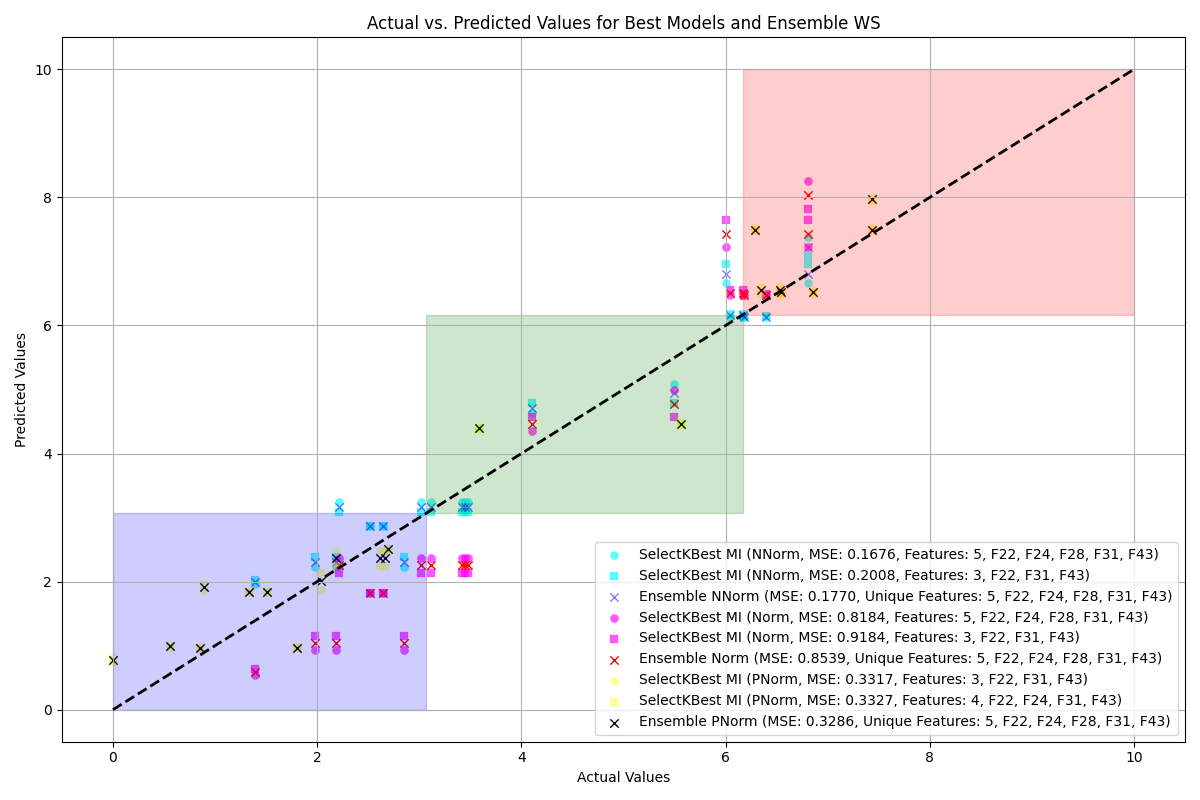
\includegraphics[width=1\linewidth]{reg_section_all/featred_ensemble_learning/actual_vs_predicted_best_feature_selection_and_ensemble_WS_10.png}
    \caption{SR Non-Norm Feature Reduction}
    \label{reg_all_fig:ws_featred_big}
\end{figure}

In this figure, the top two models and our ensemble learning for our three datasets (NNorm, Norm, PNorm) are presented.
In this figure, the classes are presented with blue, green and red squares for lower, moderate and higher ratings.
We can observe how the normalization has an important effect on the results when comparing NNorm against Norm and PNorm.
NNorm seems to mostly be concentrated in the moderate class while Norm and PNorm are more evenly spread out.
It also demonstrates our initial hypothesis on the reason why NNorm achieves a lower MSE than Norm and PNorm.
NNorm can cluster the prediction closely together since the range is smaller.
Nonetheless, both Norm and PNorm have achieved good results with most sites being in the correct class.
Figures \ref{reg_all_fig:pr_featred} to \ref{reg_all_fig:sfst_ben_featred} in the annex show the graphs for all \ac{EF}s.
These figure also demonstrate the difference in results with some \ac{EF}s performing very well, such as \ac{WS} while others, such as \ac{SFST} Benefit, did not.
However, most of our \ac{EF}s achieved impressive results and were able to converge.

To confirm our results, we propose class grouping to compare the results with classification.
We use the lower and higher boundaries presented in section \ref{sec:data} to classify the results.
We present an overview of all three data normalization (NNorm, Norm, PNorm) in table \ref{reg_all_tab:summary_grouping}.
We also show detailed results for all three respectively in tables \ref{reg_all_tab:non_norm_accuracy}, \ref{reg_all_tab:norm_accuracy} and \ref{reg_all_tab:pre_norm_accuracy}.
We compared the class grouping using the same boundaries for all three data normalization.
Meaning the non-normalized results use the same classes as the normalized results.
This was done in order to compare the results against each other.

\begin{table}[H]
\centering
\begin{tabular}{|c||c|c||c|c||c|c|}
\hline
\multirow{2}{*}{\textbf{Function}} & \multicolumn{2}{c||}{\textbf{NNorm}} & \multicolumn{2}{c||}{\textbf{Norm}} & \multicolumn{2}{c|}{\textbf{PNorm}} \\
\cline{2-7}
 & \textbf{Overall} & \textbf{Ensemble} & \textbf{Overall} & \textbf{Ensemble} & \textbf{Overall} & \textbf{Ensemble} \\
\hline
PR & 88.10\% & 90.48\% & 76.19\% & 76.19\% & 78.57\% & 76.19\% \\
\hline
SR & 80.95\% & 88.10\% & 85.71\% & 85.71\% & 85.71\% & 83.33\% \\
\hline
NR & 85.71\% & 85.71\% & 85.71\% & 71.43\% & 88.10\% & 76.19\% \\
\hline
WS & 85.71\% & 73.81\% & 90.48\% & 90.48\% & 90.48\% & 90.48\% \\
\hline
SFST & 90.48\% & 90.48\% & 88.10\% & 88.10\% & 88.10\% & 88.10\% \\
\hline

PR Benefit & 80.95\% & 80.95\% & 85.71\% & 83.33\% & 90.48\% & 90.48\% \\
\hline
SR Benefit & 97.62\% & 92.86\% & 92.86\% & 92.86\% & 95.24\% & 90.48\% \\
\hline
NR Benefit & 90.48\% & 92.86\% & 78.57\% & 83.33\% & 92.86\% & 92.86\% \\
\hline
WS Benefit & 78.57\% & 78.57\% & 80.95\% & 80.95\% & 80.95\% & 83.33\% \\
\hline
SFST Benefit & 83.33\% & 83.33\% & 80.95\% & 80.95\% & 83.33\% & 83.33\% \\
\hline
\end{tabular}
\caption{Summary of Overall and Ensemble Accuracy for Non-Normalized, Normalized, and Pre-Normalized Data for Class Grouping}
\label{reg_all_tab:summary_grouping}
\end{table}



When looking at the summary in table \ref{reg_all_tab:summary_grouping}, PNorm seems to be the most promising normalization method.
In fact, NNorm achieved an accuracy of 87.38\%, Norm achieved 84.99\% and PNorm achieved 87.62\%.
NNorm achieving similar classification results as PNorm is unexpected.
Initially we assumed NNorm would perform the worst since it was not normalized with the classification bounds.
Nonethless, it achieved bvery impressive results with a range of classifcation fromm 85.71\% to 97.62\%.
PNorm achieved a larger range from 78.57\% to a maximum of 95.24\%.
More impressive is the possibility of NNorm to classify \ac{NR} with an accuracy of 90.48\% compared to 78.57\% using PNorm.
When looking at the global accuracy, meaning the highest for each \ac{EF}, we achieved an overall accuracy of 89.53\%.


Table \ref{reg_all_tab:best} shows the best model for each \ac{EF} with the MSE, overall accuracy and features used.

\begin{table}[H]
\centering
\begin{tabular}{|c|p{3cm}|c|c|c|c|c|}
\hline
\textbf{Function} & \textbf{Model/Data} & \textbf{MSE} & \textbf{Accuracy} & \textbf{Features} & \textbf{Figures}  \\
\hline
 PR & NNorm, Ensemble & 0.3807 & 90.48\% & F43, F44, F45 & \ref{reg_all_fig:pr_featred} \\
\hline
 SR & PNorm, AdaBoost, KNN & 0.8303 & 88.10\% & F24, F28, F29, F44 & \ref{reg_all_fig:sr_featred} \\
\hline
 NR & PNorm, AdaBoost, KNN & 0.7361 & 85.71\% & F24, F43, F44, F45 & \ref{reg_all_fig:nr_featred} \\
\hline
 WS & PNorm, AdaBoost, Custom & 0.4642 & 90.48\% & F22, F31, F43 & \ref{reg_all_fig:ws_featred}\\
\hline
 SFST &  PNorm & 0.5688 & 88.10\% &  F43, F44 & \ref{reg_all_fig:sfst_featred}\\
\hline
 PR Benefit & PNorm, MLP, FFill & 1.3627 & 90.48\% & F14, F41, F43, OF19 & \ref{reg_all_fig:pr_ben_featred}\\
\hline
SR Benefit & PNorm, AdaBoost, FFill & 2.0620 & 95.24\% &  F41, OF19, OF21& \ref{reg_all_fig:sr_ben_featred}\\
\hline
 NR Benefit & PNorm, MLP, KNN & 3.4702 & 92.86\% & F14, OF9, OF10, OF19 & \ref{reg_all_fig:nr_ben_featred}\\
\hline
 WS Benefit & PNorm, AdaBoost, Mean & 0.9022 & 8095\% & Hydrogeo., OF17, OF23, OF24  & \ref{reg_all_fig:ws_ben_featred}\\
\hline
 SFST Benefit & PNorm & 2.3641 & 83.33\% & F43, F44 & \ref{reg_all_fig:sfst_ben_featred} \\
\hline
\end{tabular}
\caption{Empty Table with 6 Columns: Function, Model/Data, MSE, Accuracy, and Features}
\label{reg_all_tab:best}
\end{table}



\clearpage
\subsection{Specific Features}
\subsubsection{Training Results}
Table \ref{reg_spec_tab:mse_summary} show a summary of our training results.
In order, this table show NNorm, Norm and PNorm for all \ac{EF}s functions and benefits.
With the exception of \ac{SFST} Benefit, all \ac{EF}s performed well and achieved a good perfomance.
In fact, we achieved MSE ranging from 0.01 to 0.16 when excluding \ac{SFST} Benefit, which achieved 1.66.
When comparing the data normalization, NNorm achieved the overall best performance, closely followed by PNorm.
Norm achieved a higher MSE than NNorm and PNorm and most \ac{EF}s with a few exception.
Certain \ac{EF}s achieved a better MSE using NNorm while others performed better using PNorm.
\ac{PR} Benefit excelled using any normalization and achieved an MSE of 0.01 across all normalization.
Overall, the Benefit scores for \ac{NR}, \ac{SR} and \ac{PR} achieved a better MSE than its function counterpart.
When compared against table \ref{reg_all_tab:mse_summary}, which uses all features, we achieved significantly better results.
We comparing all \ac{EF}s, we achieved an average MSE of 0.359, 0.520 and 0.402 for all features while specific features achieved 0.295, 0.614 and 0.960 for NNorm, Norm and PNorm respectively.
However due to \ac{SFST} Benefit achieving an abnormally high MSE, we verified the results using the median and by it.
In terms of median, we achieved 0.22, 0.45 and 0.31 using all features while we achieved 0.10, 0.19, 0.24 using specific features.
When removing \ac{SFST} Benefit, we achieved averages of 0.312, 0.469, 0.367 using all features while specific features achieved 0.142, 0.211 and 0.137.
These results demonstrate two things, first it demonstrates how a single outlier can skew the perception of our results.
At first glance using the averages, all features performed better than specific features.
However, when removing the outlier the specific features significantly outperformed using all features.
These results also shiw that \ac{SFST} Benefit is missing important features in the specific dataset to infer their score.
Our specific features achieved lower results for both classification and regression for \ac{SFST} Benefit.
It highlights our reasoning for using all features rather than only using specific features.
The WESP-AC may only require specific features to calculate the score while \ac{ML} may require different ones.
Nonetheless, our results using only specific features are highly promising with most \ac{EF}s achieving low MSE.



\begin{table}[H]
\centering
\begin{tabular}{|c|c|c|c|}
\hline
\textbf{Feature} & \textbf{Non-Normalized MSE} & \textbf{Normalized MSE} & \textbf{Pre-Normalized MSE} \\
\hline
NR & 0.15 & 0.43 & 0.24 \\
\hline
PR & 0.11 & 0.18 & 0.24 \\
\hline
SR & 0.08 & 0.13 & 0.27 \\
\hline
SFST & 0.16 & 0.26 & 0.20 \\
\hline
WS & 0.10 & 0.19 & 0.08 \\
\hline
NR Benefit & 0.08 & 0.09 & 0.07 \\
\hline
PR Benefit & 0.01 & 0.01 & 0.01 \\
\hline
SR Benefit & 0.07 & 0.09 & 0.01 \\
\hline
SFST Benefit & 1.66 & 3.22 & 4.37 \\
\hline
WS Benefit & 0.53 & 0.54 & 0.11 \\
\hline
\end{tabular}
\caption{Summary of Best MSE for Non-Normalized, Normalized, and Pre-Normalized Data}
\label{reg_spec_tab:mse_summary}
\end{table}


In the annex, figure \ref{reg_spec_tab:norm_mse} show the full results for the NNorm and Norm while  figure \ref{reg_spec_tab:pre_norm_mse} show PNorm.
In these table we show which model and data filling method the results were achieved with.
The AdaBoost regressor has achieved the overall best results and was used for most \ac{EF}s.
Most filling methods performed similarly with no clear benefit of using a specific one.
However, our custom filling was the most popular with seven appearance while mean, iterative or KNN appeared three times each.
We assume our custom method, which used -1, enabled our models to know the value was missing.
Using methods that infer missing value may confuse the model by using wrong values while using -1 may enable the model to infer it by itself.
In futur iterations of our work it could be interesting to use different custom methods.
It would also be interesting to use different filling methods for different features.
Features that are only missing sporadically could use method such as iterative while mostly missing features could use our custom approach.

We also implemented ensemble learning using the specific features dataset.
Table \ref{reg_spec_tab:ensemble} show the results of ensemble learning.
In this table, each normalization method is presented with and without ensemble learning.
Similar to previous sections, ensemble learning did not seem to benefit the models.
In fact, in most instances the MSE was increased when using ensemble learning.
Norm benefited from ensmeble learning the most with some \ac{EF}s achieving lower MSE with ensemble learning.
However, the reduction in MSE is not significant since it only by a few 0.01.



\begin{table}[H]
\centering
\begin{tabular}{|c||c|c|c||c|c|c|}
\hline
\multirow{2}{*}{\textbf{Feature}} & \multicolumn{3}{c||}{\textbf{Specific}} & \multicolumn{3}{c|}{\textbf{Ensemble}} \\
\cline{2-7}
 & \textbf{Non-Norm} & \textbf{Norm} & \textbf{Pre-Norm} & \textbf{Non-Norm} & \textbf{Norm} & \textbf{Pre-Norm} \\
\hline
PR &  0.11 & 0.18 & 0.24 & 0.10 & 0.16 & 0.24\\
\hline
NR &  0.15 & 0.43 & 0.24 & 0.14 & 0.40 & 0.22 \\
\hline
SR &  0.08 & 0.13 & 0.27 & 0.07 & 0.11 & 0.18\\
\hline
WS & 0.10 & 0.19 & 0.08 & 0.06 & 0.11 & 0.13\\
\hline
SFST &  0.16 & 0.26 & 0.20 & 0.17 & 0.29 & 0.20\\
\hline
PR Benefit & 0.01 & 0.01 & 0.01 & 0.23 & 0.01 & 0.0.\\
\hline
NR Benefit &  0.08 & 0.09 & 0.07 & 0.11 & 0.12 & 0.04\\
\hline
SR Benefit &  0.07 & 0.09 & 0.01 & 0.12 & 0.09 & 0.02\\
\hline
WS Benefit &  0.53 & 0.54 & 0.11 & 0.54 & 0.55 & 0.09 \\
\hline
SFST Benefit & 1.66 & 3.22 & 4.37 & 1.90 & 3.61 & 4.40\\
\hline
\end{tabular}
\caption{Ensemble Learning for Specific Features}
\label{reg_spec_tab:ensemble}
\end{table}


In the annexe, figures \ref{reg_spec_fig:pr_ensemble} to \ref{reg_spec_fig:sfst_ben_ensemble} show the predictions with the classes.
When looking at the overall behavior of these figures, we can see that all three normalization performed well.
Pnorm achieved better results than Norm as expected with PNorm being closer to the actual values.
NNorm achieved beater results than PNorm for functions while it achieved slightly lower results for benefits.
Figure \ref{reg_spec_fig:ws_ensemble_big} below show the ensemble learning graph for \ac{WS}.
In this figure, we can see how well our algorithms performed using any normalization.

\begin{figure}[h]
    \centering
    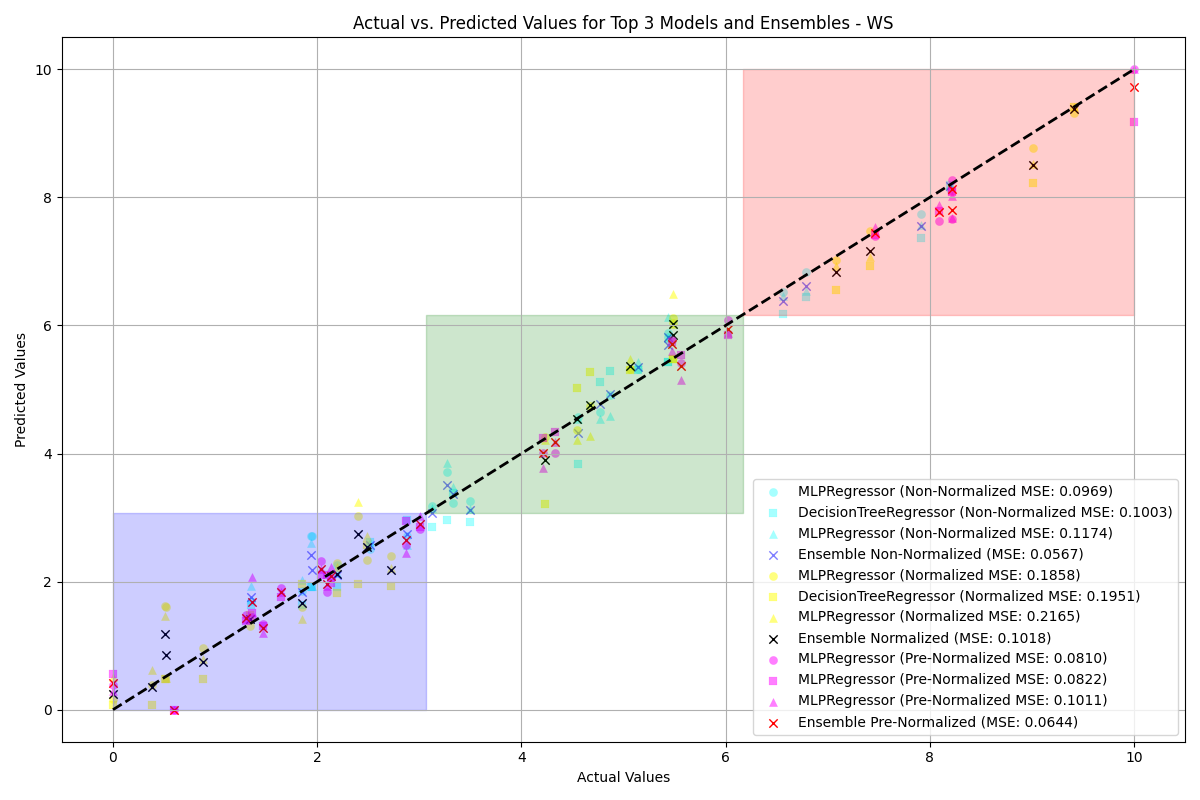
\includegraphics[width=0.95\linewidth]{reg_section_specific/ensemble_learning/actual_vs_predicted_top_3_models_and_ensembles_WS.png}
    \caption{WS Graphs Specific Features}
    \label{reg_spec_fig:ws_ensemble_big}
\end{figure}

Most sites, using Norm or PNorm, were within an MSE score of one or less.
This figure also demonstrates how good our regression predictions can be for class grouping.
Table \ref{reg_spec_tab:summary_class_grouping} show the class grouping while tables \ref{reg_spec_tab:non_norm_accuracy}, \ref{reg_spec_tab:norm_accuracy} and \ref{reg_spec_tab:pre_norm_accuracy} show the detailed results.

\begin{table}[H]
\centering
\begin{tabular}{|c||c|c||c|c||c|c|}
\hline
\multirow{2}{*}{\textbf{Function}} & \multicolumn{2}{c||}{\textbf{NNorm}} & \multicolumn{2}{c||}{\textbf{Norm}} & \multicolumn{2}{c|}{\textbf{PNorm}} \\
\cline{2-7}
 & \textbf{Overall} & \textbf{Ensemble} & \textbf{Overall} & \textbf{Ensemble} & \textbf{Overall} & \textbf{Ensemble} \\
\hline
PR & 90.48\% & 92.86\% & 78.57\% & 76.19\% & 90.48\% & 90.48\% \\
\hline
SR & 85.71\% & 85.71\% & 80.95\% & 76.19\% & 92.86\% & 92.86\% \\
\hline
NR & 88.10\% & 85.71\% & 80.95\% & 71.43\% & 100.00\% & 95.24\% \\
\hline
WS & 90.48\% & 90.48\% & 97.62\% & 97.62\% & 95.24\% & 90.48\% \\
\hline
SFST & 90.48\% & 90.48\% & 88.10\% & 88.10\% & 97.62\% & 97.62\% \\
\hline
PR Benefit & 92.86\% & 90.48\% & 92.86\% & 92.86\% & 88.10\% & 88.10\% \\
\hline
SR Benefit & 92.86\% & 85.71\% & 90.48\% & 83.33\% & 100.00\% & 100.00\% \\
\hline
NR Benefit & 92.86\% & 92.86\% & 92.86\% & 92.86\% & 88.10\% & 88.10\% \\
\hline
WS Benefit & 78.57\% & 78.57\% & 80.95\% & 85.71\% & 92.86\% & 90.48\% \\
\hline
SFST Benefit & 71.43\% & 66.67\% & 52.38\% & 52.38\% & 50.00\% & 52.38\% \\
\hline
\end{tabular}
\caption{Summary of Overall and Ensemble Accuracy for Non-Normalized (NNorm), Normalized (Norm), and Pre-Normalized (PNorm) Data for Class Grouping}

\label{reg_spec_tab:summary_class_grouping}
\end{table}

The overall results in table \ref{reg_spec_tab:summary_class_grouping} show promising results.
NNorm performed very well when considered it does not normalize the data and the boundaries were generated using the normalization sites.
In fact, it achieved better results on most \ac{EF}s than the Norm data.
PNorm achieved the best results for seven of the ten \ac{EF}s with the remaining three being close.
In fact NNorn, Norm and PNorm respectively achieved an average overall accuracy of 87.083\%, 83.472\% and 89.426\%.
Impressively, NNorm achieved a classification accuracy of 71.43\% on \ac{SFST} Benefit.
When excluding \ac{SFST} Benefit, our data normalization techniques achieved 89.155\% , 87.038\% and 93.925\%.
These results are similar to using classification directly on the specific features.
However with regression we are able to directly predict the score which is more beneficial.




\subsubsection{Feature Reduction}
Using the best performing model for each normalization technique, we perform feature reduction.
We used the same three techniques as the previous sections.
Table \ref{reg_spec_tab:featred_res} show the best models with a maximum of five features.

\begin{table}[H]
\centering
\begin{tabular}{|c|c|c|p{2.5cm}|c|p{2.5cm}|}
\hline
\textbf{\ac{EF}} & \textbf{NNorm} & \textbf{Norm} & \textbf{Features} & \textbf{PNorm} & \textbf{Features} \\
\hline
PR & 0.2463 & 0.3916 & F24, F28, F43, F44, F45 & 1.0651 & F28, F43, F44, F45 \\
\hline
SR & 0.5499 & 0.9251 & F28, F29, F31, F43, F44 & 1.3284 & F28, F31, F44 \\
\hline
NR & 0.2879 & 0.7066 & F1, F24, F43, F44, F45 & 0.0850 & F43, F44 \\
\hline
WS & 0.0838 & 0.1665 & F22, F28, F31, F43 & 0.8815 & F22, F28, F31, F43, F44 \\
\hline
SFST & 0.2208 & 0.3715 & F1, F14, F24, F43 & 0.6496 & F1, F43 \\
\hline
PR\_Benefit & 0.7844 & 0.8554 & F41, OF19, OF20, OF21, OF24 & 0.3265 & F41, OF19, OF20, OF21, OF22 \\
\hline
NR\_Benefit & 2.6496 & 3.0701 & F41, OF10, OF19, OF9 & 0.8918 & F41, OF10, OF19, OF21, OF9 \\
\hline
SR\_Benefit & 2.5425 & 2.3806 & F41, OF19 & 0.1807 &  F41, OF19, OF21 \\
\hline
WS\_Benefit & 0.6022 & 0.6119 & F51, OF17, OF18, OF23, OF24 & 2.1603 & F51, OF17, OF23, OF24, OF8 \\
\hline
SFST\_Benefit & 2.2402 & 4.3334 & OF22, OF25, OF28 & 9.8386 & F50, OF22, OF25, OF28 \\
\hline
\end{tabular}
\caption{Best MSE with Corresponding Features}
\label{reg_spec_tab:featred_res}
\end{table}

In this table, we show each \ac{EF} with both the NNorm and Norm MSE with their respective features while PNorm show the same.
In comparison with using all specific features on Functions, our reduced features achieved slightly higher MSEs.
Our Benefit scores performed poorlu using reduced features.
Usgin NNorm, \ac{PR} Benefit was increased from 0.01 to 0.7844 while \ac{NR} Benefit was increases to 2.6496 from 0.08.
Compared to feature reduction using all features in table \ref{reg_all_tab:featred_res}, reduced specific features performed Using NNorm, \ac{WS} achieved an MSE of 0.0838 using four features while it achieved 0.2627 using four features in table \ref{reg_all_tab:featred_res}.
This could be caused by the model having too much data which hinders the ability to learn.
Nonetheless, our overall results demonstrates that using specific features can be beneficial over using all features.

Our ensemble learning results did not increase our performance and often increased the MSE.
In the annex, we show our ensemble learning results in figures  \ref{reg_spec_fig:pr_featred} to \ref{reg_spec_fig:sfst_ben_featred}.
They show our validation predictions for the top two models and the ensemble approach for all three normalizations.
A glaring issue is the normalized predictions which seems to have a larger error margin.
This makes sense since htye are the NNorm predictions scaled which means the errors are also scaled.
Nonethless we achieved good grouping such as in figure \ref{reg_spec_fig:nr_featred_big} where three distinct clusters can be seen for Norm and PNorm.
A cluster near the lower-moderate boundary, near the moderate-higher boundary and in the higher class can be seen.
This demonstrates that our approach can cluster regression prediction into classes well.

\begin{figure}
    \centering
    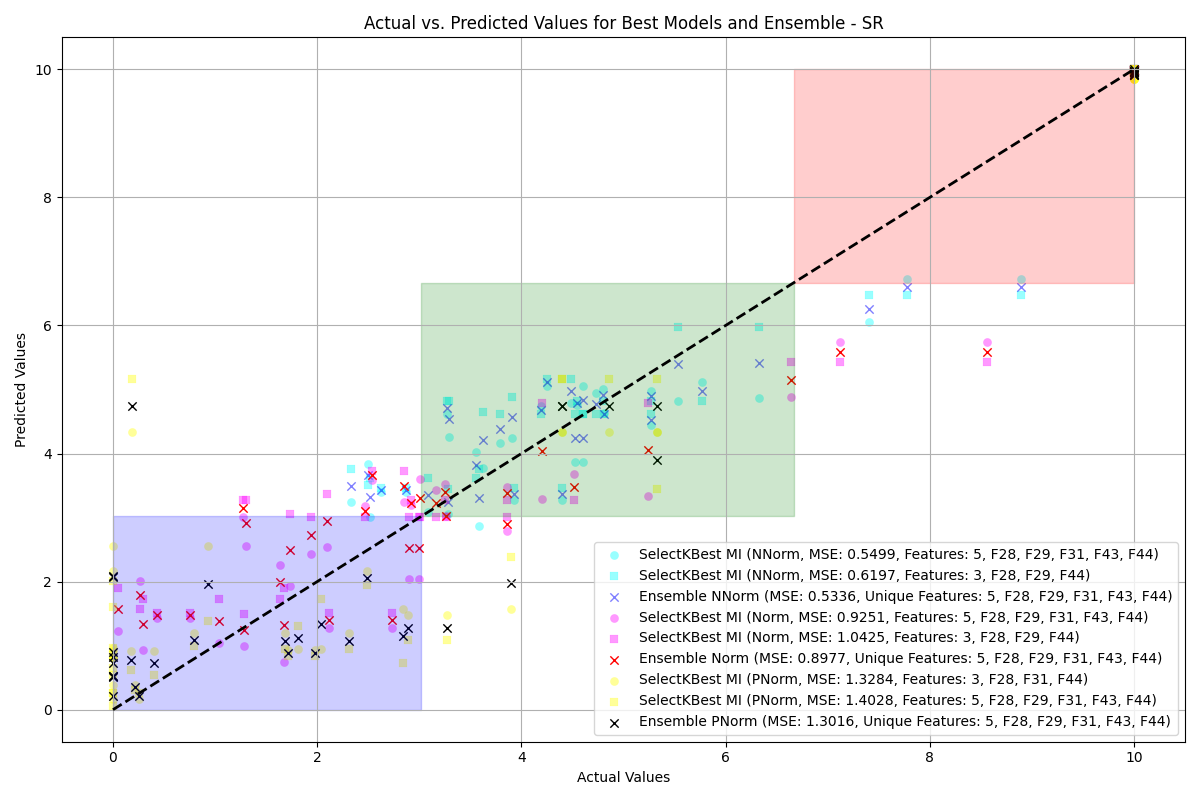
\includegraphics[width=1\linewidth]{reg_section_specific/featred_ensemble_learning/actual_vs_predicted_best_feature_selection_and_ensemble_SR_10.png}
    \caption{NR Graphs Specific Features}
    \label{reg_spec_fig:nr_featred_big}
\end{figure}


These results are confirmed in table \ref{reg_spec_tab:summary_grouping} which show a summary of our class grouping.

\begin{table}[H]
\centering
\begin{tabular}{|c||c|c||c|c||c|c|}
\hline
\multirow{2}{*}{\textbf{Function}} & \multicolumn{2}{c||}{\textbf{NNorm}} & \multicolumn{2}{c||}{\textbf{Norm}} & \multicolumn{2}{c|}{\textbf{PNorm}} \\
\cline{2-7}
 & \textbf{Overall} & \textbf{Ensemble} & \textbf{Overall} & \textbf{Ensemble} & \textbf{Overall} & \textbf{Ensemble} \\
\hline
WS & 90.48\% & 90.48\% & 97.62\% & 97.62\% & 95.24\% & 90.48\% \\
\hline
PR & 90.48\% & 92.86\% & 78.57\% & 76.19\% & 90.48\% & 90.48\% \\
\hline
NR & 88.10\% & 85.71\% & 80.95\% & 71.43\% & 100.00\% & 95.24\% \\
\hline
SR & 85.71\% & 85.71\% & 80.95\% & 76.19\% & 92.86\% & 92.86\% \\
\hline
SFST & 90.48\% & 90.48\% & 88.10\% & 88.10\% & 97.62\% & 97.62\% \\
\hline
PR Benefit & 92.86\% & 90.48\% & 92.86\% & 92.86\% & 88.10\% & 88.10\% \\
\hline
SR Benefit & 92.86\% & 85.71\% & 90.48\% & 83.33\% & 100.00\% & 100.00\% \\
\hline
NR Benefit & 92.86\% & 92.86\% & 92.86\% & 92.86\% & 88.10\% & 88.10\% \\
\hline
WS Benefit & 78.57\% & 78.57\% & 80.95\% & 83.33\% & 92.86\% & 90.48\% \\
\hline
SFST Benefit & 71.43\% & 66.67\% & 52.38\% & 54.76\% & 50.00\% & 52.38\% \\
\hline
\end{tabular}
\caption{Summary of Overall and Ensemble Accuracy for Non-Normalized (NNorm), Normalized (Norm), and Pre-Normalized (PNorm) Data for Class Grouping}
\label{reg_spec_tab:summary_grouping}
\end{table}


In this table we show the overall classification accuracy for each normalization for both the top approach and ensemble.
PNorm achieved the overall best accuracy of 89.39\% while NNorm and Norm achieved 87.38\% and 83.33\% respectively.
Compared to using all specific features, we slightly decreased the performance.
Using all features we achieved 89.426\%, 87.083\% and 83.472\% while we achieved 89.39\%,  87.38\% and 83.33\% for PNorm, NNorm and Norm respectively.
To handle the \ac{SFST} Benefit outlier problem, we compared the averages wtihout it.
PNorm achieved the best at 92.41\% while NNorm and nNorm respectively achieved 89.16\% and 87.37\%.
These results were comparable to using all features whcih achieved 93.925\%, 89.155\% and 87.138\%.
However due to the significant decrease in features used, using reduced specific features achieved impressive results.
We achieved similar results on all \ac{EF}s while using a portion of the specific features.


Tables \ref{reg_spec_tab:featred_non_norm_accuracy}, \ref{reg_spec_tab:featred_norm_accuracy} and \ref{reg_spec_tab:featred_pre_norm_accuracy} show detailed results.
In these tables we show the lower, moderate and higher accuracies of NNorm, Norm and PNorm respectively.
These tables provide us with information such as a lack of sites in the validation dataset.
Having an equal amount of site for each rating would be beneficial.



Table \ref{reg_spec_tab:best} show the best results for the Specific Features dataset.
\begin{table}[H]
\centering
\begin{tabular}{|c|p{3cm}|c|c|p{3cm}|c|}
\hline
\textbf{Function} & \textbf{Model/Data} & \textbf{MSE} & \textbf{Accuracy} & \textbf{Features} & \textbf{Figures}  \\
\hline
 PR & PNorm, AdaBoost, Iterative & 1.0651 & 90.48\% & F28, F43, F44, F5 &\ref{reg_spec_fig:pr_featred} \\
\hline
 SR & PNorm, MLP, Custom & 1.3284 & 92.86\% & F28, F31, F44 & \ref{reg_spec_fig:sr_featred} \\
\hline
 NR & PNorm, AdaBoost, Iterative & 0.0850 & 100.00\% & F43, F44 & \ref{reg_spec_fig:nr_featred} \\
\hline
 WS & Norm, MLP, Mode & 0.1665 & 97.62\% & F22, F28, F31, F43 & \ref{reg_spec_fig:ws_featred}\\
\hline
 SFST & PNorm, AdaBoost, Mean & 0.6496 & 97.62\% & F1, F43 & \ref{reg_spec_fig:sfst_featred}\\
\hline
 PR Benefit & PNorm, MLP, Median & 0.3265 & 92.86\% & F41, OF19, OF20, OF21, OF22 & \ref{reg_spec_fig:pr_ben_featred}\\
\hline
SR Benefit & Pnorm, DecisionTree, Median & 0.1807 & 100.00\% & F41, OF19, OF21 & \ref{reg_spec_fig:sr_ben_featred}\\
\hline
 NR Benefit & PNorm, MLP, Custom & 0.8918 & 92.86\% & F41, OF9, OF10, OF19, OF21 & \ref{reg_spec_fig:nr_ben_featred}\\
\hline
 WS Benefit & PNorm, DecisionTree, Mean & 2.1603 & 92.86\% & F51, OF8, OF17, OF23, OF24 & \ref{reg_spec_fig:ws_ben_featred}\\
\hline
 SFST Benefit & NNorm, RANSAC, Interpolated & 2.2402 & 71.43\% & OF22, OF25, OF28 & \ref{reg_spec_fig:sfst_ben_featred} \\
\hline
\end{tabular}
\caption{Best Models Using Specific Features}
\label{reg_spec_tab:best}
\end{table}

In this table we present which model for each \ac{EF} acheved the best MSE and accuracy with reduced features.
Excluding \ac{SFST} Benefit, we achieved a range of accuracies from 90.48\% to 100.00\% using two to five features.
This amount of features is a considerable improvement from using all or even ust speciofic features.
\ac{NR}, qhich usually requires 33 features, was reduced to using only two features to achieved 100.00\% accuracy.
Similarly, \ac{SR} Benefit achieved an accuracy of 100.00\% using only three features.
These results are highly impressive since we only used \~ 200 sites for training.
However, more training would be required since 100.00\% should not be taken as a perfect model.
Furthermore, using PNorm limits our models to use only sites which can be normalized using the same calibration sites.
Our NNorm data also achieved good results with a slightly lower accuracy with similar amount of features.
These results dmeonstarte that we can both use normalized, non-normalized and pre-normalized results.
Each method has their benefit and can be used for specific situations dpeneding on the requirements.






\clearpage





\section{Detailed Analysis of \ac{EF}s using \ac{ML}}
In this section we discuss our findings for different \ac{EF}s separately.
Table \ref{tab:combined_summary} presents the best results for both classification and regression using all and specific features. 

\begin{longtable}{|p{2cm}|p{1.5cm}|p{1.5cm}|p{3.5cm}|p{1.5cm}|p{3.5cm}|}
\hline
\textbf{Function} & \textbf{Type} & \multicolumn{2}{c|}{\textbf{All Features}} & \multicolumn{2}{c|}{\textbf{Specific Features}} \\
\cline{3-6}
 & & \textbf{Acc.} & \textbf{Features} & \textbf{Acc.} & \textbf{Features} \\
\hline
\endfirsthead

\hline
\textbf{Function} & \textbf{Type} & \multicolumn{2}{c|}{\textbf{All Features}} & \multicolumn{2}{c|}{\textbf{Specific Features}} \\
\cline{3-6}
 & & \textbf{Acc.} & \textbf{Features} & \textbf{Acc.} & \textbf{Features} \\
\hline
\endhead

PR & Class. & 85.71\% & F43, F45 & 85.71\% & F43, F45 \\
\cline{2-6}
 & Reg. & \textbf{90.48\%} & \textbf{F43, F44,} F45 & 90.48\% & F28, F43, F44, F5 \\
\hline
SR & Class. & 80.95\% & Hydrogeo., F24, F29, F43, F44, F45 & 71.42\% & OF22, F35, F43, F45, F49 \\
\cline{2-6}
 & Reg. & 88.10\% & F24, F28, F29, F44 & \textbf{92.86\%} & \textbf{F28, F31, F44} \\
\hline
NR & Class. & 80.95\% & F43, F44 & 80.95\% & F43, F44, F45 \\
\cline{2-6}
 & Reg. & 85.71\% & F24, F43, F44, F45 & \textbf{100.00\%} & \textbf{F43, F44} \\
\hline
WS & Class. & 90.45\% & F43, F46 & 85.71\% & F43, F44 \\
\cline{2-6}
 & Reg. & 90.48\% & F22, F31, F43 & \textbf{97.62\%} &\textbf{ F22, F28, F31, F43} \\
\hline
SFST & Class. & 95.24\% & F43, F44 & 95.24\% & F1, F43 \\
\cline{2-6}
 & Reg. & 88.10\% & F43, F44 &\textbf{ 97.62\%} & \textbf{F1, F43} \\
\hline
PR Benefit & Class. & 90.45\% & F14, F24, F41, F43, F46, F47 & 85.71\% & OF22, F41 \\
\cline{2-6}
 & Reg. & 90.48\% & F14, F41, F43, OF19 & \textbf{92.86\%} & \textbf{F41, OF19, OF20, OF21, OF22 }\\
\hline
SR Benefit & Class. & 100.00\% & OF19, OF21, F41, F43 & 95.24\% & OF19, F41 \\
\cline{2-6}
 & Reg. & 95.24\% & F41, OF19, OF21 & \textbf{100.00\%} & \textbf{F41, OF19, OF21} \\
\hline
NR Benefit & Class. & 90.45\% & MossCover, OF9, OF10, OF19, F1, F14, F41, F43 & 90.48\% & OF9, OF10, OF19, OF21, F41 \\
\cline{2-6}
 & Reg. & \textbf{92.86\%} & \textbf{F14, OF9, OF10, OF19} & 92.86\% & F41, OF9, OF10, OF19, OF21 \\
\hline
WS Benefit & Class. & \textbf{95.24\%} & \textbf{OF17, OF23} & 95.24\% & OF17, OF24, F51 \\
\cline{2-6}
 & Reg. & 80.95\% & Hydrogeo., OF17, OF23, OF24 & 92.86\% & F51, OF8, OF17, OF23, OF24 \\
\hline
SFST Benefit & Class. & 80.95\% &  F43, F44 & 57.14\% & OF22, OF28 \\
\cline{2-6}
 & Reg. & \textbf{83.33\%} & \textbf{F43, F44 }& 71.43\% & OF22, OF25, OF28 \\
\hline
\caption{Combined Summary of Accuracy and Features for Classification and Regression, Including Benefits}
\label{tab:combined_summary}
\end{longtable}
In this table, the most pertinent model for each \ac{EF} are presented bolded.

\subsection{PR}
Phosphorus retention is critical for the health and biodiversity of our planet.
It consists the ability of a wetland to retain phosphorus for long periods of time.
Farms can increase the nearby quantity of phosphorus which can negatively impact surrounding wetlands.
Monitoring the ability of a wetland to retain phosphorus can provide better insight on land management.
PR is one of the most demanding \ac{EF} with 22 features required from the WESP-AC for the \ac{FS} and 11 for Benefit.
By reducing the required amount of features to evaluate a site, it could greatly help researchers.
When looking at table \ref{tab:combined_summary}, \ac{PR} achieved promising results for \ac{FS}.
We achieved similar scores from both all features and specific features.
The features used for classification and regression were similar for both datasets.
In fact, \ac{PR} used both F43 and F45 to achieve an accuracy of 85.71\% using either datasets.
For regression, they achieved 90.48\% using either F43, F44 and F45 while specific features also required F28.
F43, F44 and F45 respectively define the channel connection and outflow duration, outflow confinement and through flow resistance.
We can see why these WESP-AC features have an effect on \ac{PR} since they show the ability of a wetland to keep or drain water.
By understanding how water stays or how long it does, it provides an insight on \ac{PR}.
F28 is defined as surface water annual fluctuation which determines how much, in cm, the water level changes.
Changing water level can be an indicator of water drainage or water filling of the wetland.
Overall these four features have an important effect on the results of \ac{PR} \ac{FS}.



Phosphorus retention can be highly beneficial to human populace by maintaining the quality of receiving waters.
The PR Benefit consists of evaluating how beneficial a wetland is for PR to humans.
A site may be highly effective for phosphorus retention but it may not be beneficial to humans and vice-versa.
PR Benefit utilizes 11 features and only shares one features with PR: OF22.
By only sharing one feature it shows how different \ac{FS} and \ac{BS} are.
Looking at the overview table, we can see that \ac{PR} \ac{BS} required more features than \ac{FS}.
In fact, the best performing model required five features while we only needed three for \ac{FS}.
Using regression with specific features, we achieved our best model with accuracy of 92.86\% while using F41, OF19, OF20, OF21 and OF22.
F41 is used for tributary channels which determines if surface water enters the wetland.
This feature is directly linked to F42 and F43 since the option determines if 42 is skipped.
OF19, OF20 and OF21 are features that are used to determine the water quality, degraded water downstream and upstream while OF22 determines how big the wetland is relative to the catchment size.
These features have a clear effect on \ac{BS} since it shows the quality of the water.
A higher water quality will be more beneficial to humans while a larger wetland will process more water.
Interestingly, when using all features we achieved an accuracy of 90.48\% using four features,  F14, F41, F43 and OF19.
F14 and F43 were not used to calculate the score in the WESP-AC.
F43 being the channel connection and outflow duration makes sense to be important for \ac{BS}.
F14 is unusual since it defines the Sphagnum moss extent in the wetland.
However, phosphorus has shown to improve nitrogen uptake and retention in Sphagnum moss peat \cite{williams1999nitrogen}.
Larger extent of sphagnum moss would signify better phosphorus retention which would signify a better benefit to humans.
This feature shows the benefit of using all features rather than specific features.
By using all features we are able to determine hidden relations between the features and scores.
Overall we achieved good results for both \ac{FS} and \ac{BS} for either classification or regression.




\subsection{NR}
Nitrate Removal \& Retention is also crucial for the health of our planet.
A wetland is able to remove nitrate by converting it into nitrogen gas with limited nitrous oxide, a negative greenhouse gas.
It consists of the ability of a wetland to remove and retain nitrate from water.
This process, called denitrification, is a microbial process that is crucial for climate change.
In the WESP-AC, \ac{NR} \ac{FS} utilizes 33 features while \ac{BS} uses 14.
Similar to \ac{PR}, \ac{NR} is one of the more challenging \ac{EF} to predict.
For \ac{FS}, regression seems to be more useful in predicting the classes than classification.
In fact, we achieved an accuracy of 100.00\% using F43 and F43 with regression and specific features.
Interestingly, we only achieved 85.71\% with the same model but with using all features.
It shows that using too many features can confuse the model and not find the most optimal features.
For classification, our models performed similarly and achieved 80.95\% using F43 and F44 with all features while specific features also used F45.
F43 and F44 have a clear effect on \ac{NR} similar to \ac{PR} since it defines the water retention, filling and draining.
F24 is the portion of the area that is without surface water, which has an effect on retaining nitrate.
An area that has almost no surface water will be less capable to retain and remove nitrate than a wetland with more water.


NR is also highly beneficial to humans by maintaining the quality of receiving waters.
\ac{BS} requires 14 features with only one feature shared with \ac{FS}, being OF22.
We achieved good performance using classification or regression and either datasets.
While using specific features, regression acheived an accuracy of 92.86\% while using F41, OF9, OF10, OF19 and OF20.
Similar to \ac{PR} \ac{BS}, F41 seems to have an effect on the results due to it determining the water capcity of a wetland.
OF9, OF10, OF19 and OF20 are all used in the WESP-AC to calculate \ac{BS}.
They are used to show the nearest population center, distance to domestic wells, water quality and degraded water upstream/
These four features have a clear effect on humans when looking at nitrate remove and retention.
The WESP-AC provides more information about how these features effect humans.
While using all features, our models performed similarly and achieved slightly better results.
In fact, our regression achiebed an accuracy of 02.86\% while only using four features, F14, OF9, OF10 and OF19.
F14 is also present in these results which is interesting and shows that it clearly has an important effect on \ac{BS}.
Similar to phosphorus, Sphagnum moss  retains a significant amount of nitrate \cite{williams1999nitrogen}.
These results are further confirmed when looking at the classification results using all features in table \ref{tab:combined_summary}.
Moss cover, one of the extra features colelcted outside the WESP-AC, was used as an important feature.
We show that \ac{NR} and \ac{PR} are quite similar when calculating their respective \ac{BS}.
This makes sense since they are both the ability to retain and remove nutrients.
Futur models combining the data and predicting both scores toegther to reduces features would be inetresting.
Our regression models for both \ac{FS} and \ac{BS} seem to achieve better results than the classification.
Not only did they achieve better accuracy with fewer features, regression provides us with the score.


\subsection{SR}
Sediment Retention \& Stabilization (\ac{SR}) is the effectiveness of a wetland for intercepting and filtering inorganic sediments to enable their deposition.
It also reduces the energy waves and currents, provides help for erosion and stabilizes underlying sediments and soil.
This \ac{EF} \ac{FS} has 19 features in the WESP-AC with three OF, 15 F and one S question.
In terms of results, the prediction of \ac{FS} was more difficult than any other \ac{FS}.
In fact, using classification with specific features we only achieved an accuracy of 71.42\% while all features achieved 80.95\%.
However, using regression with specific features we achieved an accuracy of 92.86\% using F28, F31 and F44.
Similar to \ac{PR} and \ac{NR}, F44 has an important effect on \ac{FS} due to it defining where major water runoff go.
F28 and F31 are respectively the annual water fluctuation and the percentage of the water that is ponded.
Water fluctuation has a direct effect on sediment retention since more water can retain more sediment.
Similarly, a wetland with more ponded water is more efficient in retenting and stabilizing sediments.
Using all features, F24 and F29 are used in combination with F28 and F44.
F29 is used in the WESP-AC for \ac{SR} \ac{FS} and is defined as the predominant depth of the wetland.
F24, which is not used in the WESP-AC, is the area that does not contain surface water, which clearly would affect the ability of a wetland to retain sediments.
Overall our calculation of \ac{SR} \ac{FS} performs very well using regression while classificationm struggle.

For \ac{SR} \ac{BS}, the score shared only OF24 with \ac{FS}, excatly the same as \ac{PR} and \ac{NR}.
We achieved our top accuracy of 100.00\% using regression with specific features and used F41, OF19 and OF21.
These four features representing tributary channels, water quality and degraded water downstream are also all present in \ac{PR} and \ac{NR} for their \ac{BS} calculating.
These three features and OF20 seem to provide us with enough information to determine the overall benefit of \ac{PR}, \ac{NR} and \ac{SR} of a wetland.
Using all features with classification with also achieved 100.00\% but with the addition of F43
F43, which is not used in the WESP-AC, is the channel connection and outflow duration.
This feature also seems to often be used in predicting the benefit of an \ac{EF}.
In fact, it is present in all classification models using all features with the exception of \ac{WS} \ac{BS}.
Nonethless, OF19 and F41 seem to be the most important features for \ac{SR} \ac{BS}.
In terms of \ac{FS} and \ac{BS} both \ac{EF}s used different features and only share one in common, F43.

\subsection{WS}
Water Storage \& Delay (\ac{WS}) is the effectiveness for storing water or delaying the movement of surface water for either long or short period of time.
Storing water enables wetland to more effectively perform its SR, NR and PR function while also slowing down erosion.
It also provides a method to control flooding by retaining water during heavy rain seasons.
\ac{WS} \ac{FS} uses 13 features while its \ac{BS} only uses six features, the lowest amount of all \ac{EF}s.
In terms of \ac{FS} performance, we achieved our best accuracy of 97.62\% using specific features with regression.
We used F22, F28, F31 and F43 which show the percentage of the area seasonally flooded, the annual fluctuation range, the percentage of pounded water and channel connection \& outflow duration.
As per the other \ac{EF}s, F43 plays an important role in determining the ability of a wetland to store water.
Similarly, F22, F28 and F31 are all directly related to showing how often and how much the wetland is flooded, ponded or dry.
Using classification, we achieved 90.45\% using all features with F43 and F46 while specific features achieved 85.71\% using F43.
Both F43 and F44 were expected to be used since they are both used to calculate the scores.
F46 however was not used in the WESP-AC and represent if a wetland has fishes or not.
This feature indirectly show if a wetland retains water year long or just seasonally or none.
If a wetland has fishes then it retains water long enough to support their habitat.
If there is no fish then the wetland is too harsh and varying to support life.
This provides us with enough information combined with F43 to classify sites into three classes.


For the \ac{BS}, we achieved our top results using all features with classification, the only \ac{EF} which achieved its top results with classification.
Using all features we achieved an accuracy of 95.24\% with OF17 and OF23 while specific features achieved 95.24\% using OF17, OF24 and F51.
Using only OF17 and OF23 is promising since it would mean we could accurately classify wetlands without the need of visiting them since they are both OF.
OF17 shows the flood damage from non-tidal waters while OF23 is the unvegetaed surface in the contributing area.
OF17 affects \ac{WS} since flood damage means human live near by and a higher storage capacity is more beneficial to reduce floods.
This feature can show lots of information since it shows how close humans live to a wetland.
OF23 is also important since vegetation is important for water storage and erosion counter.
More vegetation means the wetland has more capabilities in \ac{WS}.
For regression, we achieved 80.95\% using the hydrogeomorphic class, OF17, OF23 and OF24 with all features while specific features achieved 92.86\% using F51, OF8, OF17, OF23 and OF24.
The model with specific features is still highly promising even if it achieved slightly lower results with two more features.
Noenthless this model would provide us with the direct score compared to the class alone.
Furthermore it only uses F51 while the others are all OF which would greatly reduce the time spent on-site.
F51 is the type of cover in a 30m which has two options, impervious (e.g parking lot) while the other is not impervious.
This feature could be done in an OF format by using satellite images rather than go on-site.
This means that were would be able to predict \ac{BS} using five OF with an accuracy of 92.86\%.
Overall, the regression results for both \ac{FS} and \ac{BS} are highly promising.
We achieved both very good accuracies with few features, with \ac{BS} using only OF.


\subsection{SFST}
Stream Flow Support (\ac{SFST}) is the effectiveness of contributing water to streams with an emphasis of bringing water to dryer parts of the area.
\ac{SFST} \ac{FS} uses 14 features while \ac{BS} only uses six features.
\ac{FS} and \ac{BS} share no common features which is interesting and showcase how different the function and benefit are.
In terms of \ac{FS}, we achieved our best results using regression with specific features.
We achieved an accuracy of 97.62\% using only F1 and F43 while using all features we achieved 88.10\% using F43 and F44.
Simialrly, classification using all features used F43 and F44 while specific features used F1 and F43.
As seen earlier, F43 and F44 are both highly important since they show channel connection, outflow duration and outflow confinenment.
It is interesting that F44 is used often in \ac{SFST} but is not present in the specific features.
F1 describes the overall vegetation, water and soil which can quickly be used to determine the \ac{SFST} function.
Overall, we achived very impressive results using classification or regression with eitehr dataset.
This \ac{EF} is the one we achieved the overall best results with.

In terms of \ac{BS}, we achieved vewry interestingly results in terms of dataset.
When using specific features, none of our classification or regression models were able to achieve good results.
Classification achieved 57.14\% using OF22 and OF28 while regression achieved 71.43\% using OFF22, OF25 and OF28.
Interestingly, the models performed well using all features and achieved regression accuracy of 83.33\% using F43 and F44.
Both of these features were not used in the WESP-AC and only F42 was used.
However, they represent channel connection \& outflow duration and outflow confinement.
This may have an effect on the benefit of \ac{SFST} since.... insert reason here.
For classification, we used the same F43 and F44 features to achieved an accuracy of 80.95\%.
\ac{SFST} \ac{BS} only using six features may cause issues with our training since too many sites may be similar.
By having similar sites with different ratings, the models may have difficulties differentiating them.
Overall \ac{FS} performed very well while we had difficulties predicting \ac{BS}.




\section{CausalML}
CausalML is a python library that combines \ac{CI} and \ac{ML}.
\ac{CI} is the process of determining whether a cause-and-effect relationship exists between variables.
Unlike correlation, which only indicates that two variables are related, causal inference seeks to understand whether changes in one variable directly cause changes in another. 
We aim to use \ac{CI} to determine which features are more or less important to certain \ac{EF}s.
Researchers could highly benefit of determining the relationship between the change in features and its effect on the \ac{EF}.
It can be combined with \ac{ML} to infer the importance of specific features.
CausalML provides tools for treatment effect estimation, propensity score modeling, uplift modeling and instrumental variables, integrating well with popular \ac{ML} libraries like scikit-learn.

We propose training similar algorithms as the classification and regression sections to determine the importance of features.
We train the algorithms using the regression D1 dataset, which included all features, for each \ac{EF}.
We compare each algorithm individually and globally using two methods to average the results.
The first is the average importance across all methods while the second is a custom point system.
The average importance consists of adding all feature importance value and average them for the number of algorithm.
In our point system, each feature is given a point based on its importance rank for each algorithm.
A feature is given the maximum amount of point for being the most important given an algorithm while its given the minimum for being last.


\subsection{Results}
We present the results in tables and graph for better visualization.
Tables \ref{tab:important_features_PR} to \ref{tab:important_features_SFST_Benefit} present the results for \ac{NR}, \ac{PR}, \ac{SR}, \ac{WS}, \ac{SFST} and their benefits respectively.
Figures \ref{fig:pr_causalml} to \ref{fig:sfst_ben_causalml} present the graphical results respectively.

Table \ref{tab:important_features_combined} show the most and least important feature for each function.

\begin{table}
\centering
\begin{tabular}{|l|l|l|l|l|}
\hline
\textbf{Function} & \textbf{Top 4 (Avg.)} & \textbf{Bottom 4  (Avg.)} & \textbf{Top 4 (Points)} & \textbf{Bottom 4 (Points)} \\
\hline
PR & \begin{tabular}[c]{@{}l@{}}'F43': 0.977784\\ 'F22': 0.075298\\ 'F49': 0.044496\\ 'F45': 0.042024\\ \end{tabular} & \begin{tabular}[c]{@{}l@{}}'F5': -0.154281\\ 'OF27': -0.046845\\ 'F6': -0.021769\\ 'OF24': -0.011727\\ \end{tabular} & \begin{tabular}[c]{@{}l@{}}'F43': 1402 points\\ 'OF22': 1231 points\\ 'F22': 1223 points\\ 'F25': 1221 points\\ \end{tabular} & \begin{tabular}[c]{@{}l@{}}'F68': 464 points\\ 'F6': 448 points\\ 'F9': 436 points\\ 'OF24': 412 points\\ \end{tabular} \\
\hline
NR & \begin{tabular}[c]{@{}l@{}}'F43': 0.612435\\ 'F45': 0.117268\\ 'F44': 0.081121\\ 'F5': 0.053705\\ \end{tabular} & \begin{tabular}[c]{@{}l@{}}'OF33': -0.006181\\ 'OF6': -0.005082\\ 'F33': -0.004765\\ 'F8': -0.004219\\ \end{tabular} & \begin{tabular}[c]{@{}l@{}}'F43': 1343 points\\ 'F45': 1220 points\\ 'F44': 1151 points\\ 'F3f': 1137 points\\ \end{tabular} & \begin{tabular}[c]{@{}l@{}}'F32': 377 points\\ 'F67': 360 points\\ 'F33': 358 points\\ 'F39': 352 points\\ \end{tabular} \\
\hline
WS & \begin{tabular}[c]{@{}l@{}}'F43': 0.951765\\ 'F5': 0.097695\\ 'F22': 0.091916\\ 'F52': 0.048698\\ \end{tabular} & \begin{tabular}[c]{@{}l@{}}'F12': -0.026529\\ 'F18': -0.020177\\ 'F62': -0.009468\\ 'OF20': -0.008094\\ \end{tabular} & \begin{tabular}[c]{@{}l@{}}'F43': 1346 points\\ 'F22': 1265 points\\ 'OF22': 1214 points\\ 'F25': 1178 points\\ \end{tabular} & \begin{tabular}[c]{@{}l@{}}'F68': 451 points\\ 'F18': 439 points\\ 'OF8': 398 points\\ 'F62': 387 points\\ \end{tabular} \\
\hline
SR & \begin{tabular}[c]{@{}l@{}}'F43': 0.563853\\ 'F45': 0.320945\\ 'F24': 0.140763\\ 'OF21': 0.114374\\ \end{tabular} & \begin{tabular}[c]{@{}l@{}}'F58': -0.013924\\ 'OF38': -0.021798\\ 'F3c': -0.026023\\ 'OF31': -0.028798\\ \end{tabular} & \begin{tabular}[c]{@{}l@{}}'F43': 1365 points\\ 'F45': 1260 points\\ 'F31': 1135 points\\ 'F24': 1130 points\\ \end{tabular} & \begin{tabular}[c]{@{}l@{}}'F21': 426 points\\ 'S2': 384 points\\ 'OF34': 377 points\\ 'OF2': 255 points\\ \end{tabular} \\
\hline

SFST & \begin{tabular}[c]{@{}l@{}}'F43': 1.039090\\ 'F5': 0.497852\\ 'OF27': 0.122599\\ 'F45': 0.035529\\ \end{tabular} & \begin{tabular}[c]{@{}l@{}}'F4': -0.014221\\ 'OF9': -0.019349\\ 'F36': -0.023610\\ 'F35': -0.027724\\ \end{tabular} & \begin{tabular}[c]{@{}l@{}}'F43': 1305 points\\ 'F1': 1149 points\\ 'F34': 1093 points\\ 'F47': 1076 points\\ \end{tabular} & \begin{tabular}[c]{@{}l@{}}'OF8': 399 points\\ 'F58': 378 points\\ 'F49': 330 points\\ 'F3g': 300 points\\ \end{tabular} \\
\hline
PR Benefit & \begin{tabular}[c]{@{}l@{}}'F41': 0.558198\\ 'OF19': 0.331069\\ 'OF21': 0.124913\\ 'F5': 0.023782\\ \end{tabular} & \begin{tabular}[c]{@{}l@{}}'OF20': -0.008562\\ 'F48': -0.004729\\ 'OF16': -0.003171\\ 'OF7': -0.003062\\ \end{tabular} & \begin{tabular}[c]{@{}l@{}}'F41': 1351 points\\ 'OF19': 1285 points\\ 'OF21': 1119 points\\ 'OF24': 1037 points\\ \end{tabular} & \begin{tabular}[c]{@{}l@{}}'F20': 424 points\\ 'F13': 472 points\\ 'F33': 478 points\\ 'OF25': 478 points\\ \end{tabular} \\
\hline
NR Benefit & \begin{tabular}[c]{@{}l@{}}'OF10': 0.417809\\ 'OF19': 0.312239\\ 'OF21': 0.205786\\ 'F41': 0.075133\\ \end{tabular} & \begin{tabular}[c]{@{}l@{}}'OF27': -0.065078\\ 'F3g': -0.014606\\ 'OF25': -0.008854\\ 'OF6': -0.007846\\ \end{tabular} & \begin{tabular}[c]{@{}l@{}}'OF10': 1342 points\\ 'OF19': 1236 points\\ 'F41': 1198 points\\ 'OF21': 1189 points\\ \end{tabular} & \begin{tabular}[c]{@{}l@{}}'F36': 356 points\\ 'OF5': 358 points\\ 'OF3': 372 points\\ 'F25': 433 points\\ \end{tabular} \\
\hline
SR Benefit & \begin{tabular}[c]{@{}l@{}}'OF19': 0.497638\\ 'F41': 0.294398\\ 'OF21': 0.268613\\ 'F12': 0.045374\\ \end{tabular} & \begin{tabular}[c]{@{}l@{}}'OF18': -0.002347\\ 'F20': -0.001792\\ 'OF5': -0.001777\\ 'OF22': -0.001403\\ \end{tabular} & \begin{tabular}[c]{@{}l@{}}'OF19': 1294 points\\ 'F41': 1231 points\\ 'OF21': 1143 points\\ 'F1': 1056 points\\ \end{tabular} & \begin{tabular}[c]{@{}l@{}}'F20': 269 points\\ 'F68': 354 points\\ 'S2': 407 points\\ 'S1': 430 points\\ \end{tabular} \\
\hline
WS Benefit & \begin{tabular}[c]{@{}l@{}}'OF17': 0.671066\\ 'F53': 0.620027\\ 'OF20': 0.235132\\ 'OF21': 0.218170\\ \end{tabular} & \begin{tabular}[c]{@{}l@{}}'F5': -0.651739\\ 'F3d': -0.161077\\ 'F3c': -0.145086\\ 'F33': -0.103096\\ \end{tabular} & \begin{tabular}[c]{@{}l@{}}'OF17': 1307 points\\ 'F52': 1237 points\\ 'OF23': 1212 points\\ 'F51': 1189 points\\ \end{tabular} & \begin{tabular}[c]{@{}l@{}}'F5': 323 points\\ 'F33': 369 points\\ 'F67': 376 points\\ 'F64': 381 points\\ \end{tabular} \\
\hline
SFST Benefit & \begin{tabular}[c]{@{}l@{}}'F43': 0.755861\\ 'F45': 0.141279\\ 'F5': 0.083083\\ 'OF28': 0.061002\\ \end{tabular} & \begin{tabular}[c]{@{}l@{}}'F3a': -0.025738\\ 'OF13': -0.020652\\ 'F3d': -0.015819\\ 'F3e': -0.012449\\ \end{tabular} & \begin{tabular}[c]{@{}l@{}}'F43': 1158 points\\ 'OF18': 1122 points\\ 'F1': 1100 points\\ 'OF28': 1080 points\\ \end{tabular} & \begin{tabular}[c]{@{}l@{}}'F20': 362 points\\ 'F22': 366 points\\ 'S2': 416 points\\ 'F62': 425 points\\ \end{tabular} \\
\hline
\end{tabular}
\caption{Features for Various Models}
\label{tab:important_features_combined}
\end{table}


\subsection{Discussion}
CausalML is a python library that implements CI and \ac{ML}.
It is often used to determine the effectivness of a treatement for a specific cause-effect relation.
However, by setting each feature as a treatement, we are able to determine how important a specific feature is to each \ac{EF}.
Tables \ref{tab:important_features_PR} to \ref{tab:important_features_SFST_Benefit} and
figures \ref{fig:pr_causalml} to \ref{fig:sfst_ben_causalml} present the numerical and graphical results, respectively.
Table \ref{tab:important_features_combined} show the most and least important feature for each function.
We also present the average importance and a voting system in the tables.
The voting system consists of providing points to each feature proportionate to how important they are when using an algorithm.
We implemented a voting system so that a specific algorithm did not have a large effect on the average importance.
The figures present both of these metrics combined for each EF.
It shows the importance of using both methods since some average importance are very small but are high in points.
Similar to our previous results using \ac{ML}, F43 seems to be highly important for most \ac{EF}s.


\clearpage
\section{Tetrad}
Tetrad is \ac{CI} modeling software that is widely used to discover causal relations between variables.
We employ this software to try to determine causal relationship between features for specific \ac{EF}s.
Our goal is to utilize the features and non-normalized score to determine relations.
However, after various algorithms, parameters and more we discovered that no model was able to fit the data.
An example of the graphical results can be seen in figure \ref{fig:tetrad}

\begin{figure}[b]
    \centering
    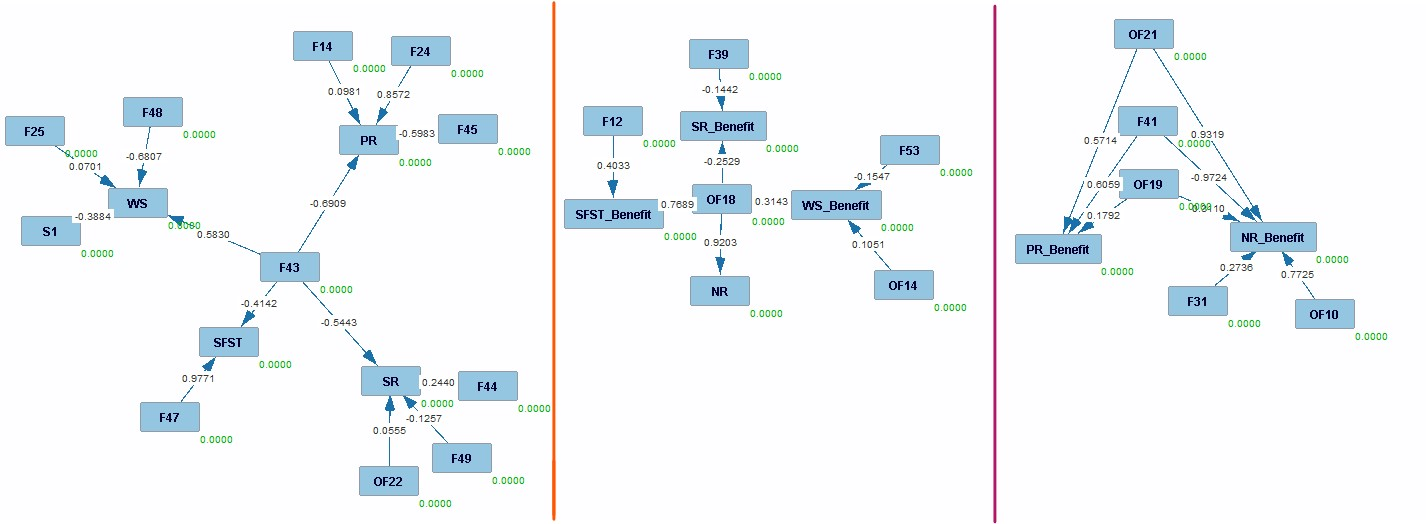
\includegraphics[width=0.95\linewidth]{tetrad/ex1.jpg}
    \caption{NR}
    \label{fig:tetrad}
\end{figure}

After multiple iterations of Tetrad yeidling no results, we turned our effort towards \ac{ML}.
Further exploration with \ac{CI} or Tetrad specialists could be beneficial in this aspect of the project.


\section{Conclusion}

\section{Future Directions}
\subsection{Data}
Our data, which consisted of 210 sites, was provided in early in mid April 2024 by Marc-Antoine from \ac{NRNB}.
It consisted of a compilation of the WESP-AC (3.3) questionnaire answers without the scores for the 210 sites.
After exploring the data and possible solutions, an important error was found.
During the calculation of the benefit score, the normalization function had possible errors.
A new version (3.4) was created to address this issue amounts others such as formatting issues.
Since the provided data was a compilation in a single csv file, a code to transfer them to the new 3.4 WESP-AC and to recalculate the results was generated.
Codes for both the scores and ratings of the explored \ac{EF}s were generated.
This gave us data to perform both regression to predict the scores and classification to classify the ratings.
We used the non-normalized scores, ranging from 0-10, and the ratings, either lower, moderate or higher.
Using non-normalized data enabled us to expand our algorithms in the future for different provinces.
Using the scores and rating data, we also removed unecessary features and filled the missing data with various methods.
This gave us nine different csv files for both the scores and ratings for this project.
Adding more data such as using the 98 reference wetlands used to normalize the WESP-AC, studying more wetlands or by using data from different provinces would highly benefit this project.
By increasing our training data, it would enable our various models to achieve better results.
This would not only give us a higher performance but it could enable us to use the data for causal inference with Tetrad.

\subsection{Classification}

\subsection{Regression}

\subsection{CausalML}

\subsection{Tetrad}




\clearpage
\bibliography{references}
\bibliographystyle{IEEEtran}


\clearpage
\section{Annexes}
\subsection{Datasets}
\begin{table}[h]
    \centering
    \begin{tabular}{|m{3cm}|c|m{11cm}|}
        \hline
        \textbf{Feature Name} & \textbf{Type} & \textbf{Description} \\
        \hline
        Provincial Class & Class (6) & This classification divides wetlands into six distinct types based on their ecological characteristics. It aids in the management and conservation of wetland resources. \\
        \hline
        Provincial Class & Class (10) & This extended classification categorizes wetlands into ten types, providing a more detailed understanding of wetland diversity for conservation strategies. \\
        \hline
        Water Regime & Class (4) & This indicator classifies water regimes into four types, describing the hydrological conditions of a wetland. It is essential for wetland management. \\
        \hline
        Vegetation Type & Class (7) & This classification identifies seven types of specific vegetation present in wetlands. It helps in assessing the ecological status of wetland areas. \\
        \hline
        Veg. Cover & Class (5) & This classification indicates the percentage cover of specific vegetation types, divided into five classes. It provides insights into vegetation distribution. \\
        \hline
        Woody Canopy & Class (4) & This classification describes the percentage cover of high woody canopy (over 5 meters), divided into four classes. It is useful for understanding forest structure in wetlands. \\
        \hline
        \% Moss Cover & Class (5) & This classification specifies the percentage cover of moss in wetlands, divided into five classes. It is important for ecological assessments. \\
        \hline
        Phragmites  & Class (3) & This feature indicates the presence of Phragmites (an invasive plant species) in a wetland, classified as yes or no. It is crucial for invasive species management. \\
        \hline
        Soil Type & Class (3) & This classification identifies the soil types in wetlands, divided into three classes. It helps in understanding soil characteristics and their impact on wetland ecology. \\
        \hline
        Surface Water & Class (7) & This classification indicates the percentage of surface water present in a wetland, divided into seven classes. It is important for hydrological studies. \\
        \hline
        Depth Sat. & Class (4) & This feature measures the depth of water saturation in soil, divided into four classes. It helps in understanding soil moisture conditions. \\
        \hline
        Depth Moss & Float & This feature measures the average depth of living moss in centimeters. It provides insights into the health and growth of moss in wetlands. \\
        \hline
        Organic Depth & Float & This feature measures the average depth of organic material in soil in centimeters. It is crucial for understanding soil composition and fertility. \\
        \hline
        Hydrogeomorphic & Class (11) & This classification divides wetlands into eleven hydrogeomorphic classes, based on their geomorphology and hydrology. It is essential for wetland characterization and management. \\
        \hline
    \end{tabular}
    \caption{Feature Descriptions for Various Wetland Attributes}
    \label{tab:data_xtra_features}
\end{table}
\clearpage
\subsection{Features}


\clearpage
\subsection{Machine Learning Algorithms}\label{sec:algorithms}
\begin{longtable}{|>{\raggedright}p{2cm}|>{\raggedright}p{3cm}|>{\raggedright\arraybackslash}p{8cm}|}
\hline
\textbf{Algorithm} & \textbf{Type} & \textbf{Parameters} \\
\hline
Ridge & Class./Reg. & 
\begin{itemize}
    \item \texttt{alpha}: [0.1, 0.5, 1.0]
    \item \texttt{solver}: ['auto', 'svd', 'cholesky', 'lsqr', 'sparse\_cg', 'sag', 'saga', 'lbfgs']
\end{itemize} \\
\hline
Decision Tree & Class./Reg. & 
\begin{itemize}
    \item \texttt{criterion}: ['gini', 'entropy', 'log\_loss'] (Class.), ['squared\_error', 'friedman\_mse', 'absolute\_error', 'poisson'] (Reg.)
    \item \texttt{splitter}: ['best', 'random']
    \item \texttt{min\_samples\_split}: [2, 3, 4, 5]
    \item \texttt{max\_features}: [None, 'sqrt', 'log2']
\end{itemize} \\
\hline
Random Forest & Class./Reg. & 
\begin{itemize}
    \item \texttt{n\_estimators}: [50, 100, 200]
    \item \texttt{criterion}: ['gini', 'entropy', 'log\_loss'] (Class.), ['squared\_error', 'friedman\_mse', 'absolute\_error', 'poisson'] (Reg.)
    \item \texttt{min\_samples\_split}: [2, 5]
    \item \texttt{max\_features}: ['sqrt', 'log2']
\end{itemize} \\
\hline
Gradient Boosting & Class./Reg. & 
\begin{itemize}
    \item \texttt{loss}: ['log\_loss', 'deviance', 'exponential'] (Class.), ['squared\_error', 'absolute\_error', 'huber', 'quantile'] (Reg.)
    \item \texttt{learning\_rate}: [0.001, 0.01, 0.1]
    \item \texttt{n\_estimators}: [50, 100, 200]
    \item \texttt{warm\_start}: [True, False]
\end{itemize} \\
\hline
AdaBoost & Class./Reg. & 
\begin{itemize}
    \item \texttt{n\_estimators}: [50, 100, 200]
    \item \texttt{learning\_rate}: [0.001, 0.01, 0.1, 1.0]
    \item \texttt{algorithm}: ['SAMME', 'SAMME.R'] (Class.), \texttt{loss}: ['linear', 'square', 'exponential'] (Reg.)
\end{itemize} \\
\hline
K-Neighbors & Class./Reg. & 
\begin{itemize}
    \item \texttt{n\_neighbors}: [5, 10, 15, 20]
    \item \texttt{weights}: ['uniform', 'distance']
    \item \texttt{algorithm}: ['auto', 'ball\_tree', 'kd\_tree', 'brute']
    \item \texttt{leaf\_size}: [30, 50, 70]
    \item \texttt{metric}: ['euclidean', 'manhattan', 'minkowski']
\end{itemize} \\
\hline
MLP (Neural Network) & Class./Reg. & 
\begin{itemize}
    \item \texttt{hidden\_layer\_sizes}: [(50, 50, 50), (100, 100, 100), (100, 100, 100, 100)]
    \item \texttt{activation}: ['identity', 'logistic', 'tanh', 'relu']
    \item \texttt{solver}: ['lbfgs', 'sgd', 'adam']
    \item \texttt{learning\_rate}: ['constant', 'invscaling', 'adaptive']
\end{itemize} \\
\hline
Logistic Regression & Classifier & 
\begin{itemize}
    \item \texttt{penalty}: ['l1', 'l2', 'elasticnet', 'none']
    \item \texttt{C}: [0.1, 0.5, 1.0, 5.0, 10.0]
    \item \texttt{solver}: ['newton-cg', 'lbfgs', 'liblinear', 'sag', 'saga']
    \item \texttt{max\_iter}: [100, 200, 300]
\end{itemize} \\
\hline
SGD & Class./Reg. & 
\begin{itemize}
    \item \texttt{loss}: ['hinge', 'log', 'modified\_huber', 'squared\_hinge', 'perceptron'] (Class.), ['squared\_error', 'huber', 'epsilon\_insensitive', 'squared\_epsilon\_insensitive'] (Reg.)
    \item \texttt{penalty}: ['l2', 'l1', 'elasticnet']
    \item \texttt{learning\_rate}: ['constant', 'optimal', 'invscaling', 'adaptive']
    \item \texttt{warm\_start}: [True, False]
\end{itemize} \\
\hline
Support Vector Machines (SVM) & Class./Reg. & 
\begin{itemize}
    \item \texttt{C}: [0.1, 1.0, 10.0]
    \item \texttt{kernel}: ['linear', 'poly', 'rbf', 'sigmoid']
    \item \texttt{degree}: [1, 3, 5]
    \item \texttt{gamma}: ['scale', 'auto']
\end{itemize} \\
\hline
Gaussian Naive Bayes & Classifier & 
\begin{itemize}
    \item \texttt{var\_smoothing}: [1e-9, 1e-8, 1e-7]
\end{itemize} \\
\hline
Linear Discriminant Analysis & Classifier & 
\begin{itemize}
    \item \texttt{solver}: ['svd', 'lsqr', 'eigen']
    \item \texttt{shrinkage}: [None, 'auto', 0.1, 0.5, 1.0]
\end{itemize} \\
\hline
ElasticNet & Regressor & 
\begin{itemize}
    \item \texttt{l1\_ratio}: [0.25, 0.5, 0.75]
    \item \texttt{fit\_intercept}: [True, False]
    \item \texttt{precompute}: [True, False]
    \item \texttt{copy\_X}: [True, False]
    \item \texttt{warm\_start}: [True, False]
    \item \texttt{positive}: [True, False]
    \item \texttt{selection}: ['cyclic', 'random']
\end{itemize} \\
\hline
Bayesian Ridge & Regressor & 
\begin{itemize}
    \item \texttt{alpha\_1}: [1e-7, 1e-6, 1e-5]
    \item \texttt{alpha\_2}: [1e-7, 1e-6, 1e-5]
    \item \texttt{lambda\_1}: [1e-7, 1e-6, 1e-5]
    \item \texttt{lambda\_2}: [1e-7, 1e-6, 1e-5]
\end{itemize} \\
\hline
Kernel Ridge & Regressor & 
\begin{itemize}
    \item \texttt{alpha}: [0.00001, 0.0001, 0.001, 0.01]
    \item \texttt{kernel}: ['linear', 'poly', 'rbf', 'sigmoid', 'precomputed']
    \item \texttt{degree}: [1, 2, 3, 5, 10]
    \item \texttt{coef0}: [0.0, 0.5, 1.0]
\end{itemize} \\
\hline
Linear Regression & Regressor & 
\begin{itemize}
    \item \texttt{fit\_intercept}: [True, False]
    \item \texttt{copy\_X}: [True, False]
    \item \texttt{positive}: [True, False]
\end{itemize} \\
\hline
RANSAC Regressor & Regressor & 
\begin{itemize}
    \item \texttt{min\_samples}: [None, 1, 2, 5, 10]
    \item \texttt{max\_trials}: [1, 10, 50, 100, 150]
    \item \texttt{loss}: ['absolute\_error', 'squared\_error']
\end{itemize} \\
\hline
Theil-Sen Regressor & Regressor & 
\begin{itemize}
    \item \texttt{max\_subpopulation}: [1, 10, 100, 500]
    \item \texttt{n\_subsamples}: [None, 1, 5, 10, 25]
\end{itemize} \\
\hline

\caption{Machine Learning Algorithms}
\label{tab:all_algorithms}
\end{longtable}

\subsection{Classification}\label{sec:class_annex}
\subsubsection{All Features}
%\begin{figure}[H]
    \centering
    \begin{minipage}[b]{0.45\textwidth}
            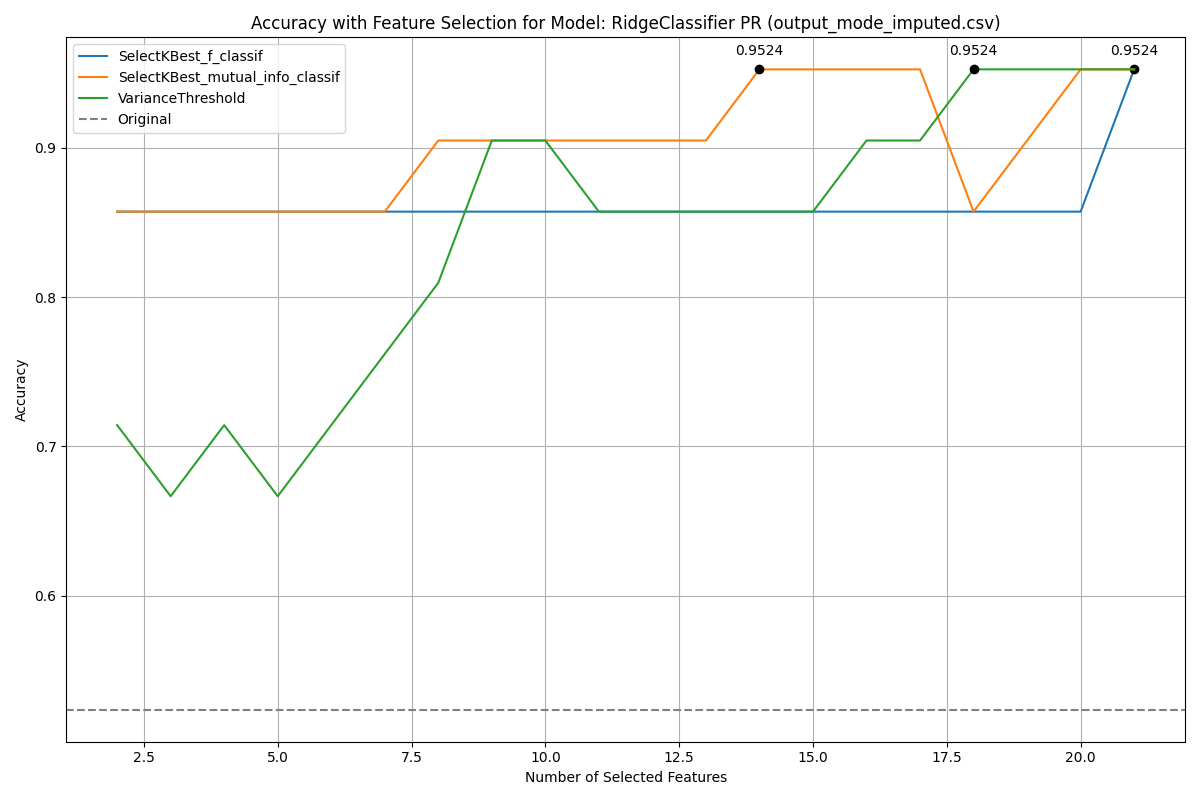
\includegraphics[width=\textwidth]{class_specific_section/images_class_ensemble_reduction/feature_selection_accuracy_plot_output_mode_imputedcsv_RidgeClassifier_PR.png}
        \caption{PR}
        \label{fig_class_spec:pr_featred_graph}
    \end{minipage}
    \hfill
    \begin{minipage}[b]{0.45\textwidth}
        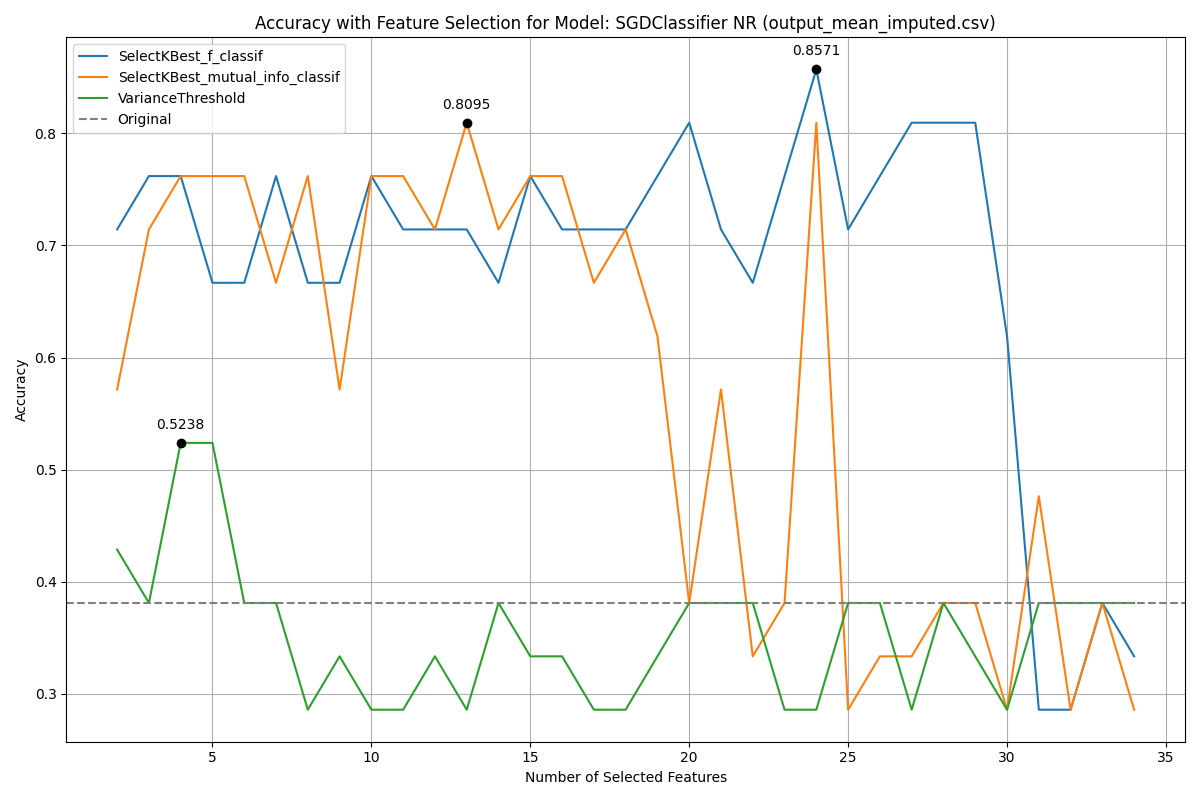
\includegraphics[width=\textwidth]{class_specific_section/images_class_ensemble_reduction/feature_selection_accuracy_plot_output_mean_imputedcsv_SGDClassifier_NR.png}
        \caption{NR}
        \label{fig_class_spec:nr_featred_graph}
    \end{minipage}
\end{figure}

\begin{figure}[H]
    \centering
    \begin{minipage}[b]{0.45\textwidth}
        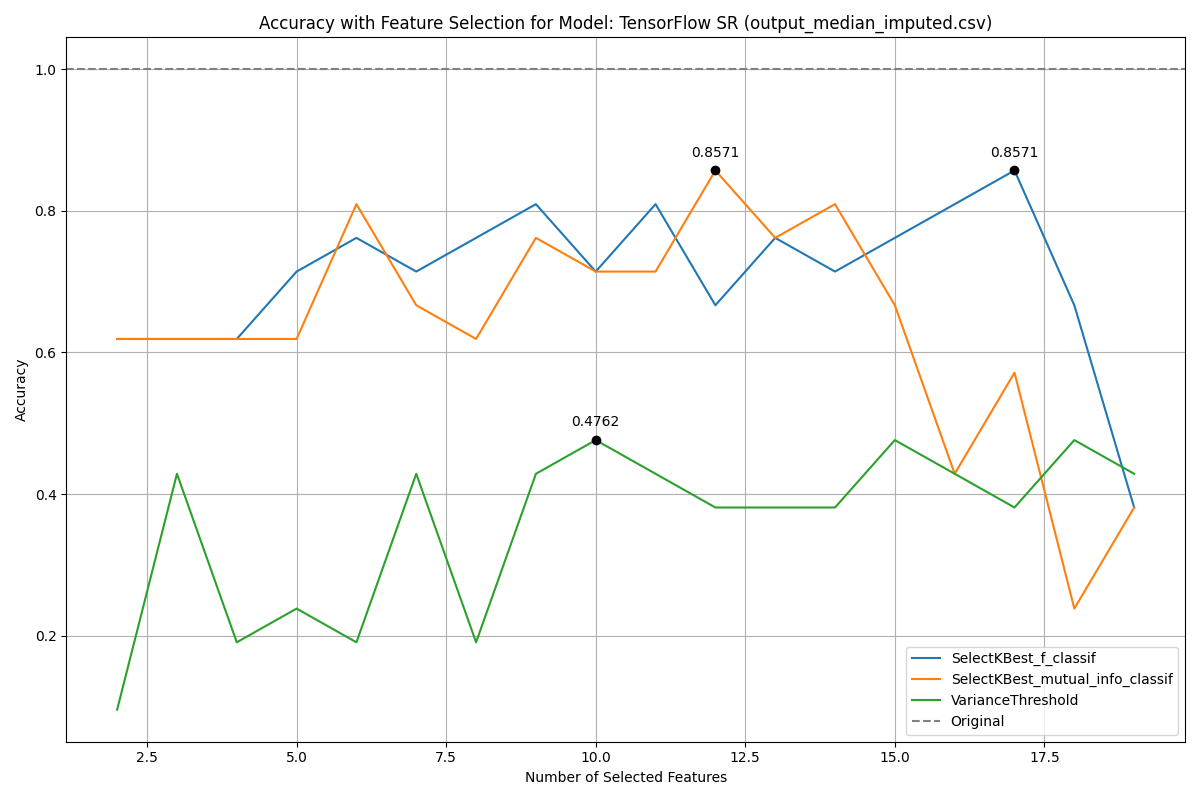
\includegraphics[width=\textwidth]{class_specific_section/images_class_ensemble_reduction/feature_selection_accuracy_plot_output_median_imputedcsv_TensorFlow_SR.png}
        \caption{SR}
        \label{fig_class_spec:sr_featred_graph}
    \end{minipage}
    \hfill
    \begin{minipage}[b]{0.45\textwidth}
        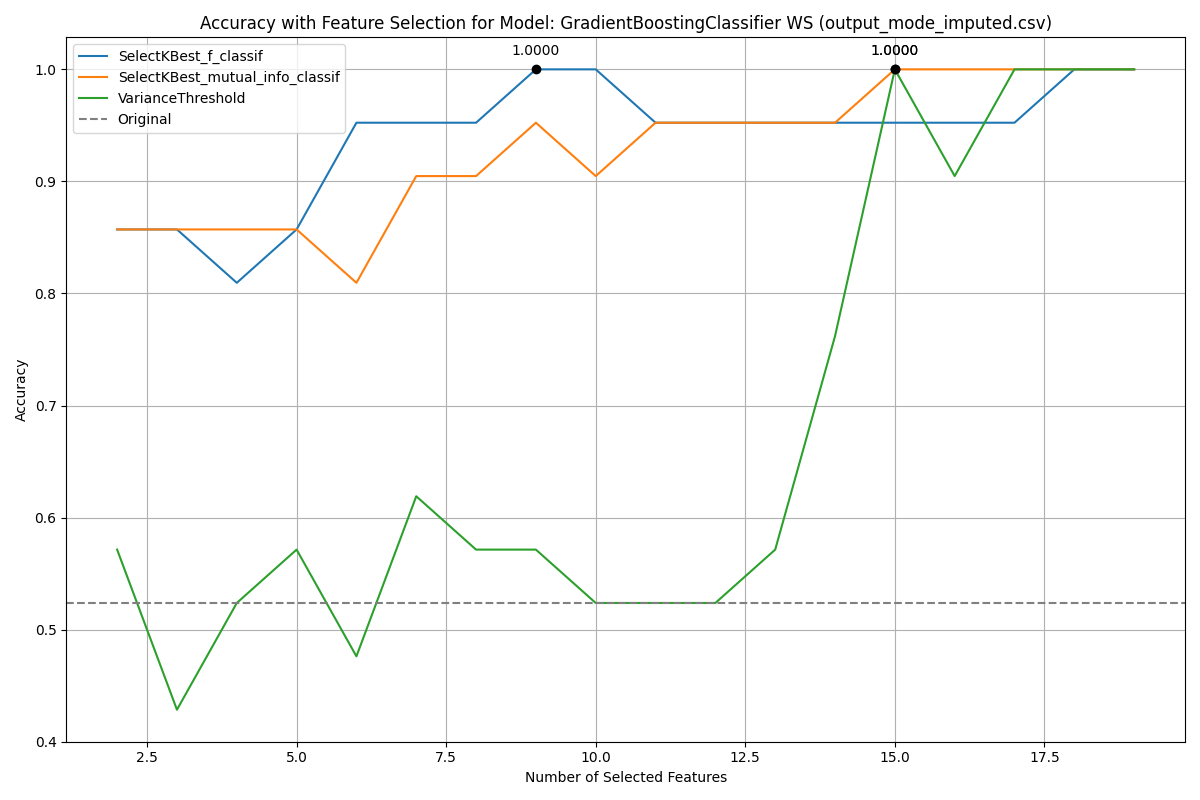
\includegraphics[width=\textwidth]{class_specific_section/images_class_ensemble_reduction/feature_selection_accuracy_plot_output_mode_imputedcsv_GradientBoostingClassifier_WS.png}
        \caption{WS}
        \label{fig_class_spec:ws_featred_graph}
    \end{minipage}
\end{figure}

\begin{figure}[H]
    \centering
    \begin{minipage}[b]{0.45\textwidth}
        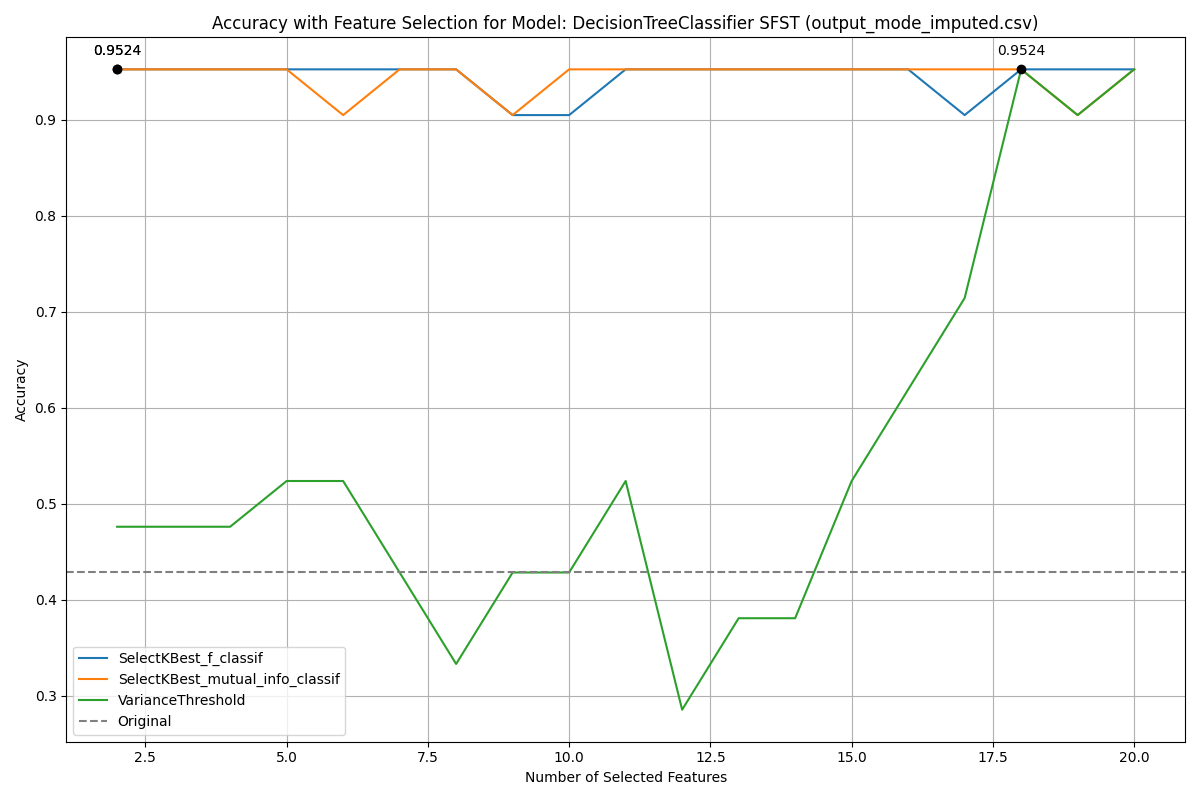
\includegraphics[width=\textwidth]{class_specific_section/images_class_ensemble_reduction/feature_selection_accuracy_plot_output_mode_imputedcsv_DecisionTreeClassifier_SFST.png}
        \caption{SFST}
        \label{fig_class_spec:sfst_featred_graph}
    \end{minipage}
    \hfill
    \begin{minipage}[b]{0.45\textwidth}
        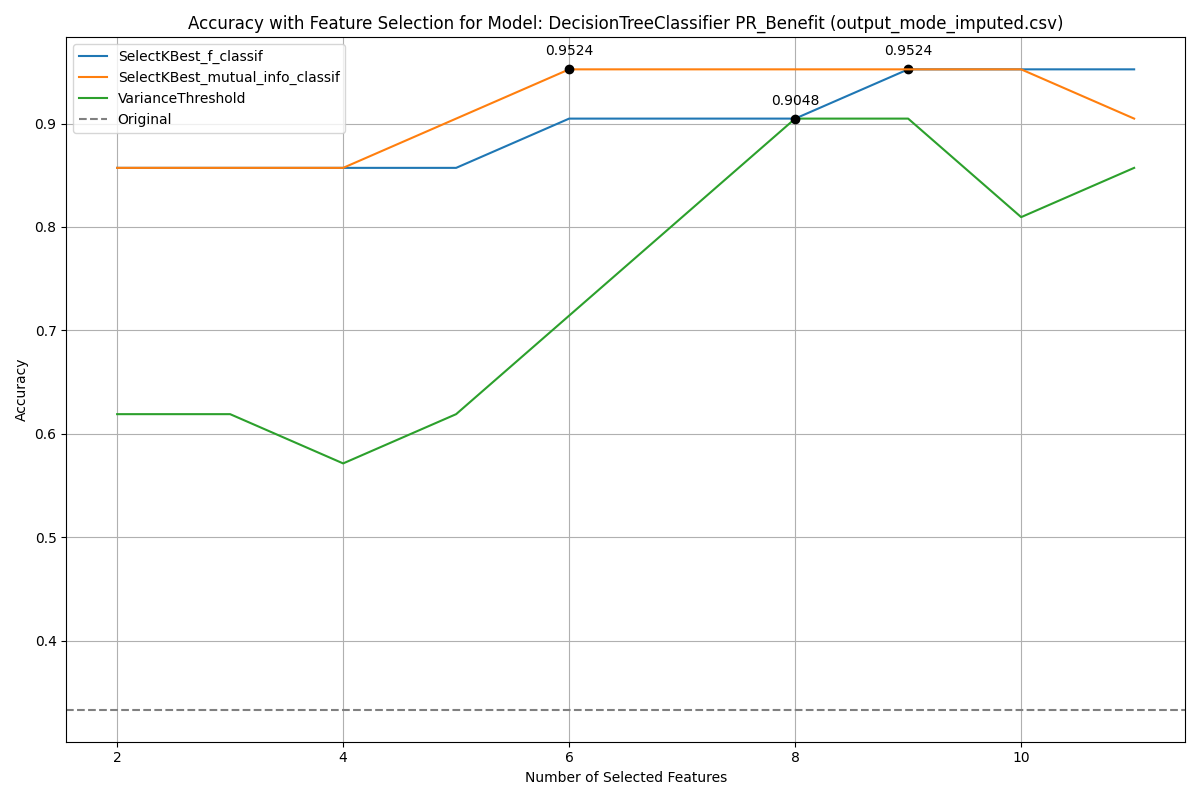
\includegraphics[width=\textwidth]{class_specific_section/images_class_ensemble_reduction/feature_selection_accuracy_plot_output_mode_imputedcsv_DecisionTreeClassifier_PR_Benefit.png}
        \caption{PR Benefit}
        \label{fig_class_spec:pr_ben_featred_graph}
    \end{minipage}
\end{figure}

\begin{figure}[H]
    \centering
    \begin{minipage}[b]{0.45\textwidth}
        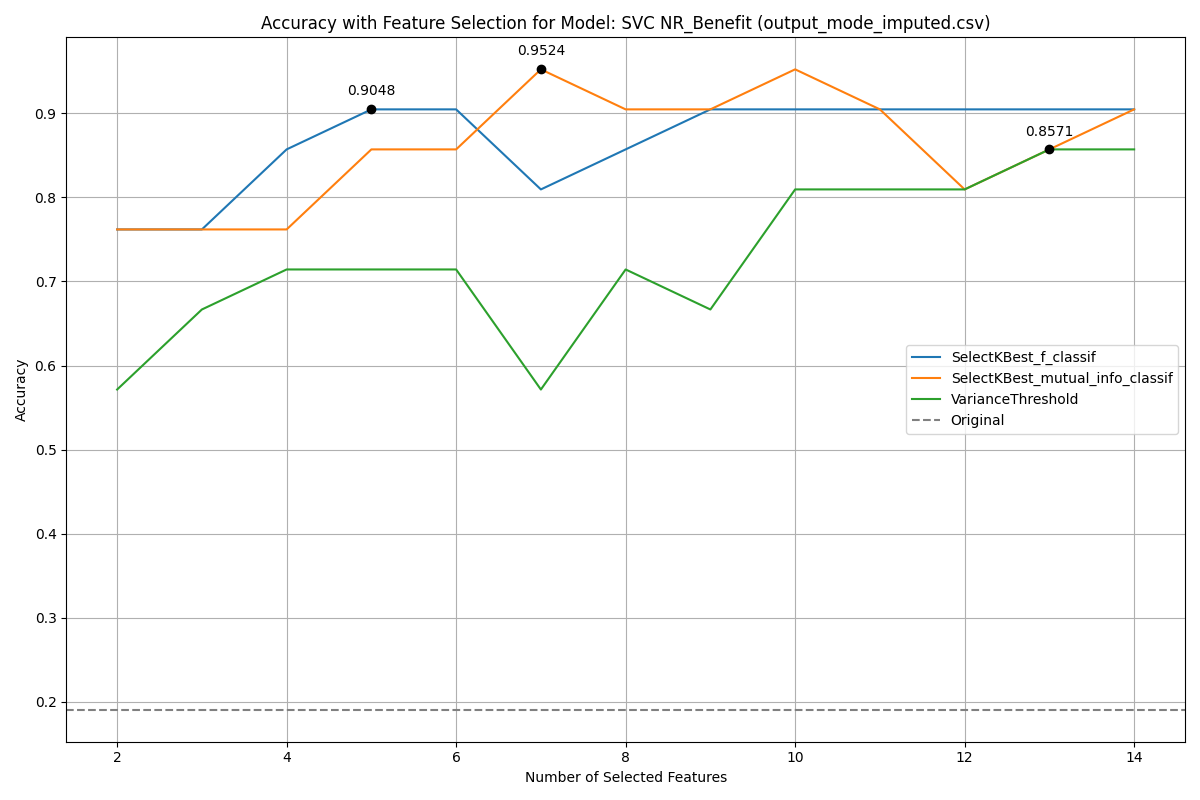
\includegraphics[width=\textwidth]{class_specific_section/images_class_ensemble_reduction/feature_selection_accuracy_plot_output_mode_imputedcsv_SVC_NR_Benefit.png}
        \caption{NR Benefit}
        \label{fig_class_spec:nr_ben_featred_graph}
    \end{minipage}
    \hfill
    \begin{minipage}[b]{0.45\textwidth}
        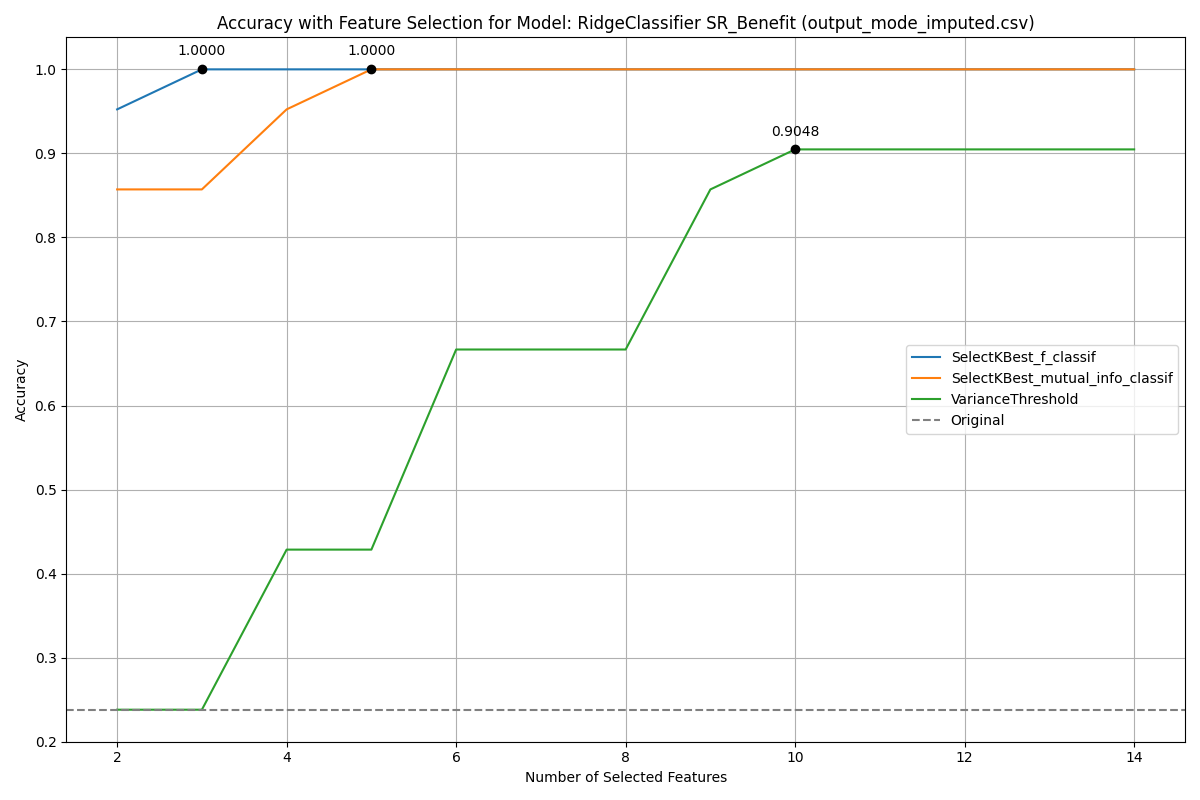
\includegraphics[width=\textwidth]{class_specific_section/images_class_ensemble_reduction/feature_selection_accuracy_plot_output_mode_imputedcsv_RidgeClassifier_SR_Benefit.png}
        \caption{SR Benefit}
        \label{fig_class_spec:sr_ben_featred_graph}
    \end{minipage}
\end{figure}

\begin{figure}[H]
    \centering
    \begin{minipage}[b]{0.45\textwidth}
        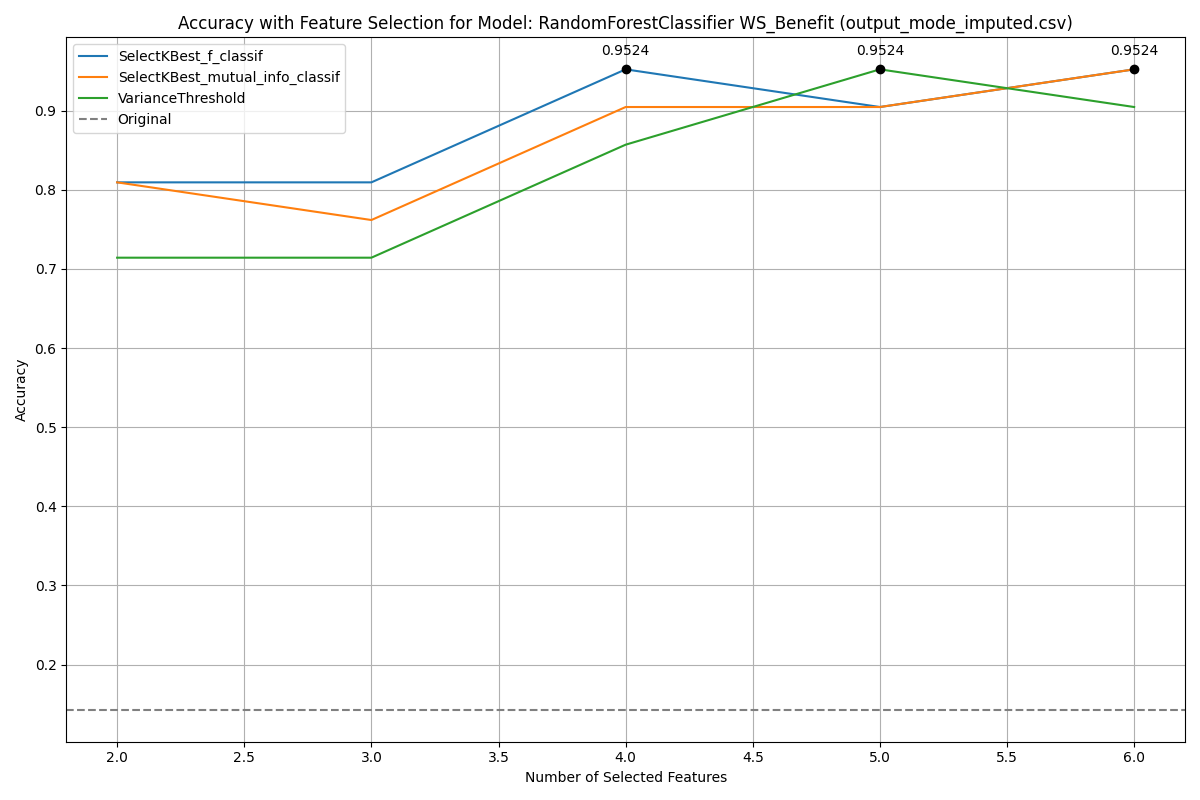
\includegraphics[width=\textwidth]{class_specific_section/images_class_ensemble_reduction/feature_selection_accuracy_plot_output_mode_imputedcsv_RandomForestClassifier_WS_Benefit.png}
        \caption{WS Benefit}
        \label{fig_class_spec:ws_ben_featred_graph}
    \end{minipage}
    \hfill
    \begin{minipage}[b]{0.45\textwidth}
        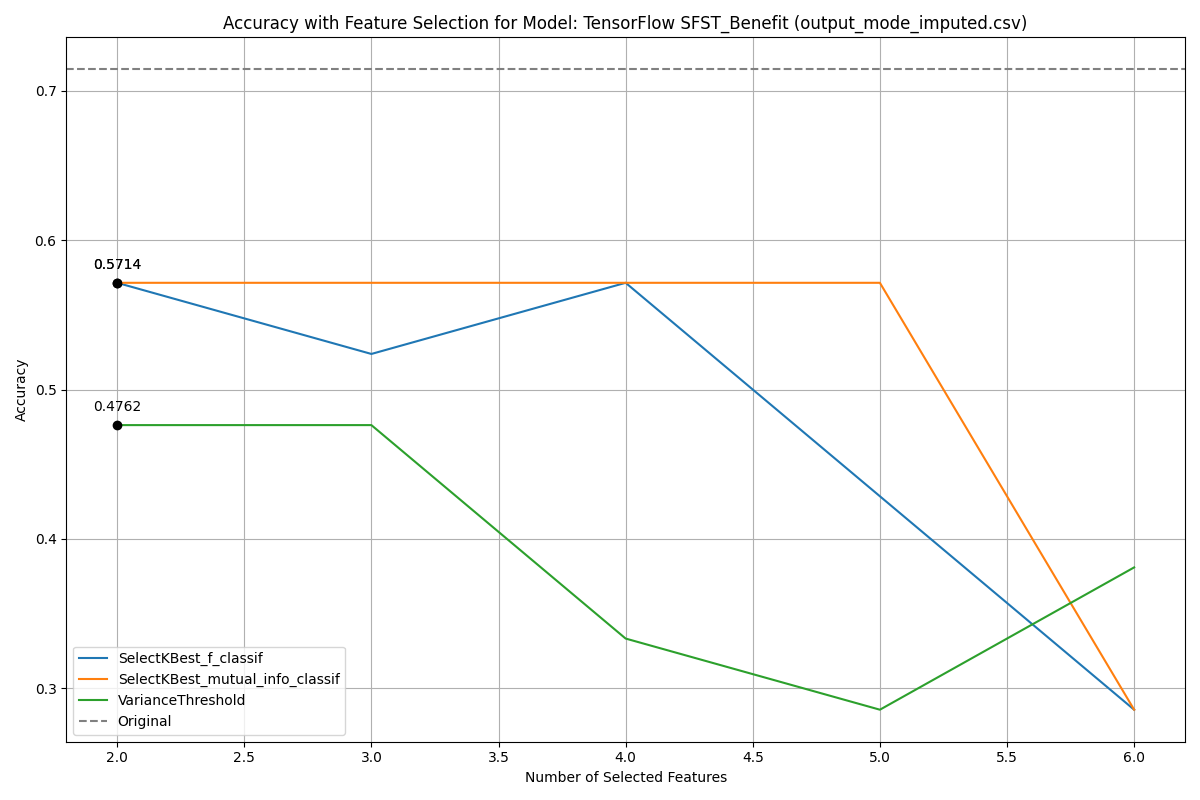
\includegraphics[width=\textwidth]{class_specific_section/images_class_ensemble_reduction/feature_selection_accuracy_plot_output_mode_imputedcsv_TensorFlow_SFST_Benefit.png}
        \caption{SFST Benefit}
        \label{fig_class_spec:sfst_ben_featred_graph}
    \end{minipage}
\end{figure}


\subsubsection{Specific Features}
%\begin{figure}[H]
    \centering
    \begin{minipage}[b]{0.45\textwidth}
            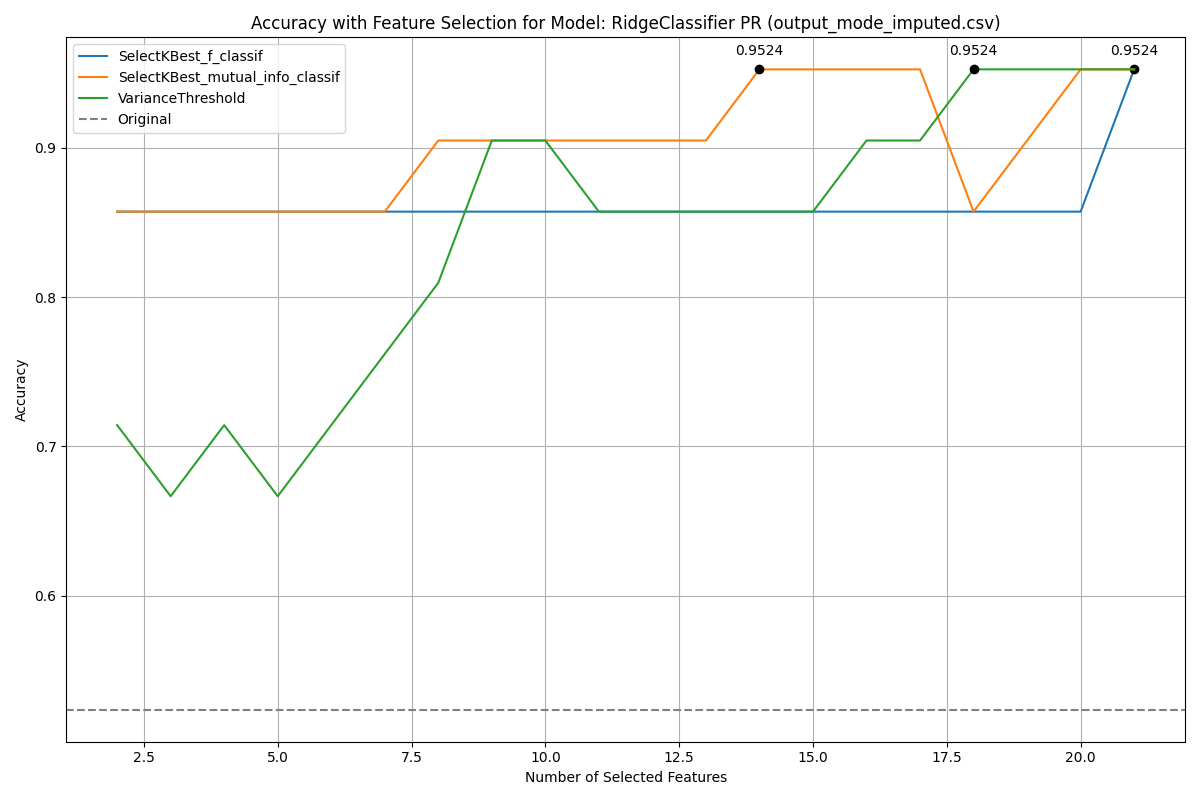
\includegraphics[width=\textwidth]{class_specific_section/images_class_ensemble_reduction/feature_selection_accuracy_plot_output_mode_imputedcsv_RidgeClassifier_PR.png}
        \caption{PR}
        \label{fig_class_spec:pr_featred_graph}
    \end{minipage}
    \hfill
    \begin{minipage}[b]{0.45\textwidth}
        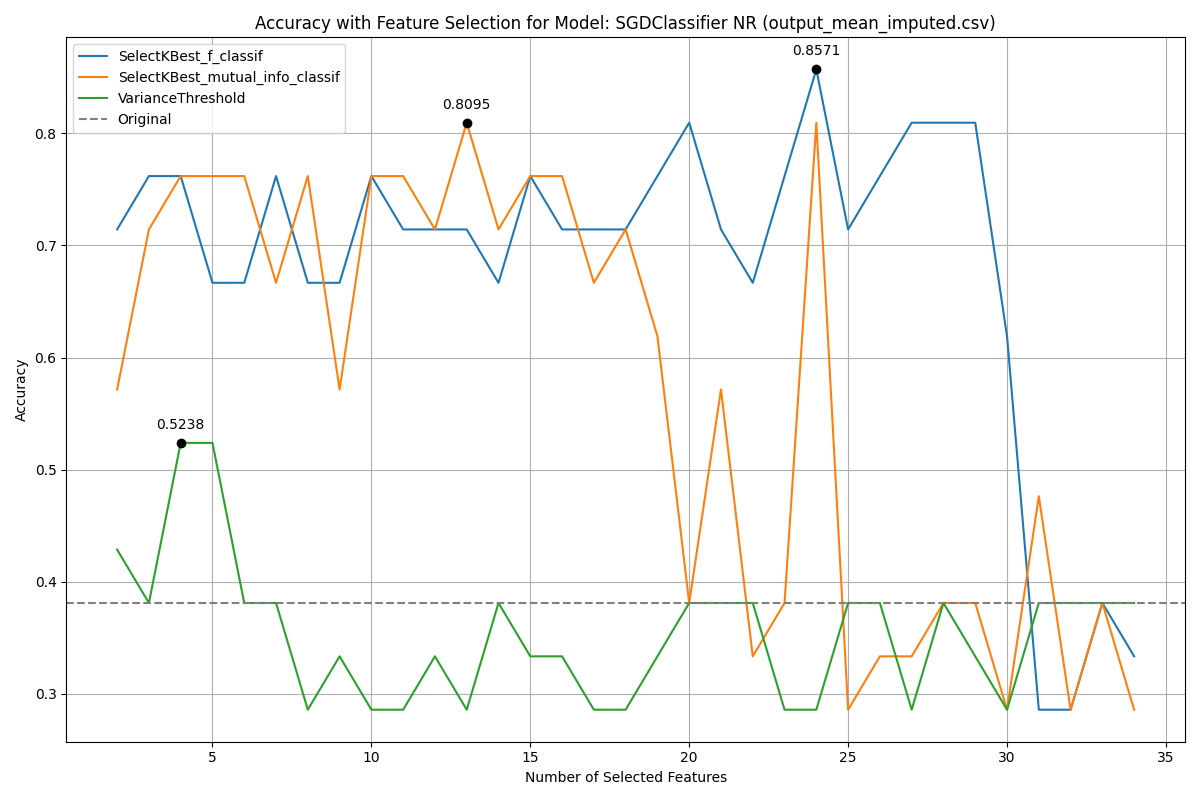
\includegraphics[width=\textwidth]{class_specific_section/images_class_ensemble_reduction/feature_selection_accuracy_plot_output_mean_imputedcsv_SGDClassifier_NR.png}
        \caption{NR}
        \label{fig_class_spec:nr_featred_graph}
    \end{minipage}
\end{figure}

\begin{figure}[H]
    \centering
    \begin{minipage}[b]{0.45\textwidth}
        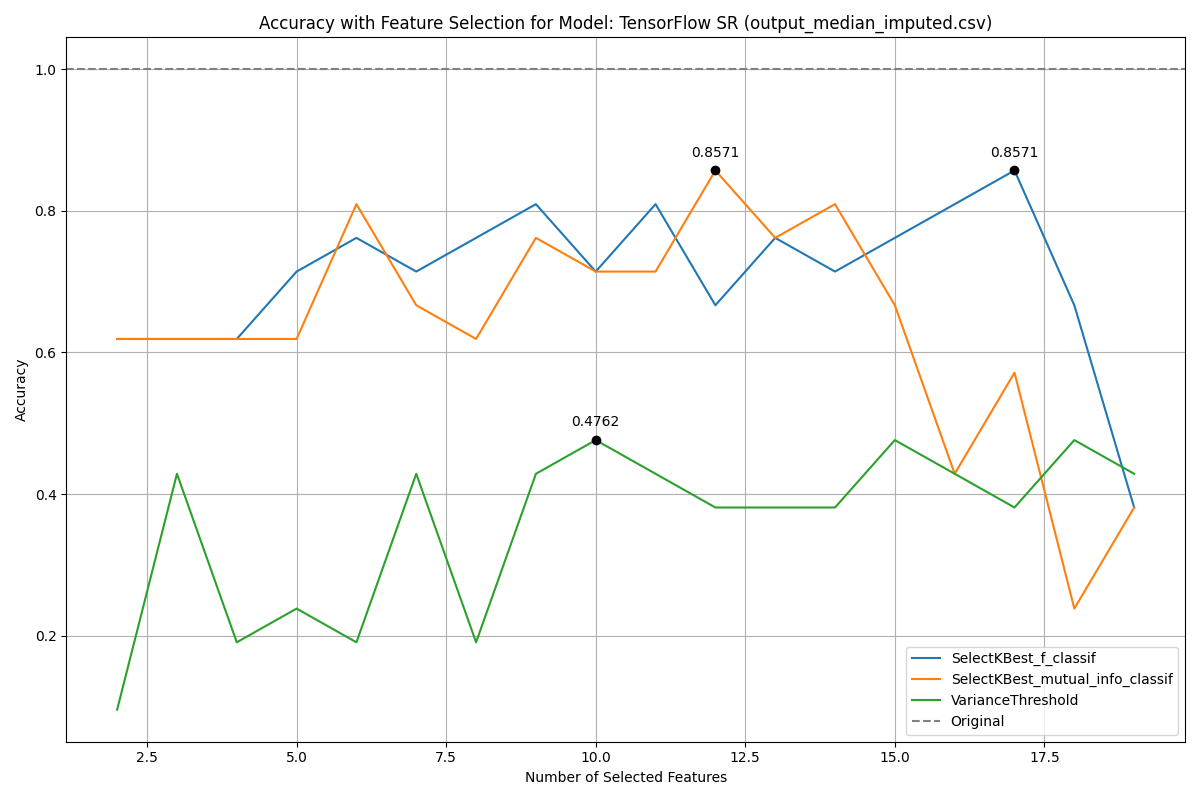
\includegraphics[width=\textwidth]{class_specific_section/images_class_ensemble_reduction/feature_selection_accuracy_plot_output_median_imputedcsv_TensorFlow_SR.png}
        \caption{SR}
        \label{fig_class_spec:sr_featred_graph}
    \end{minipage}
    \hfill
    \begin{minipage}[b]{0.45\textwidth}
        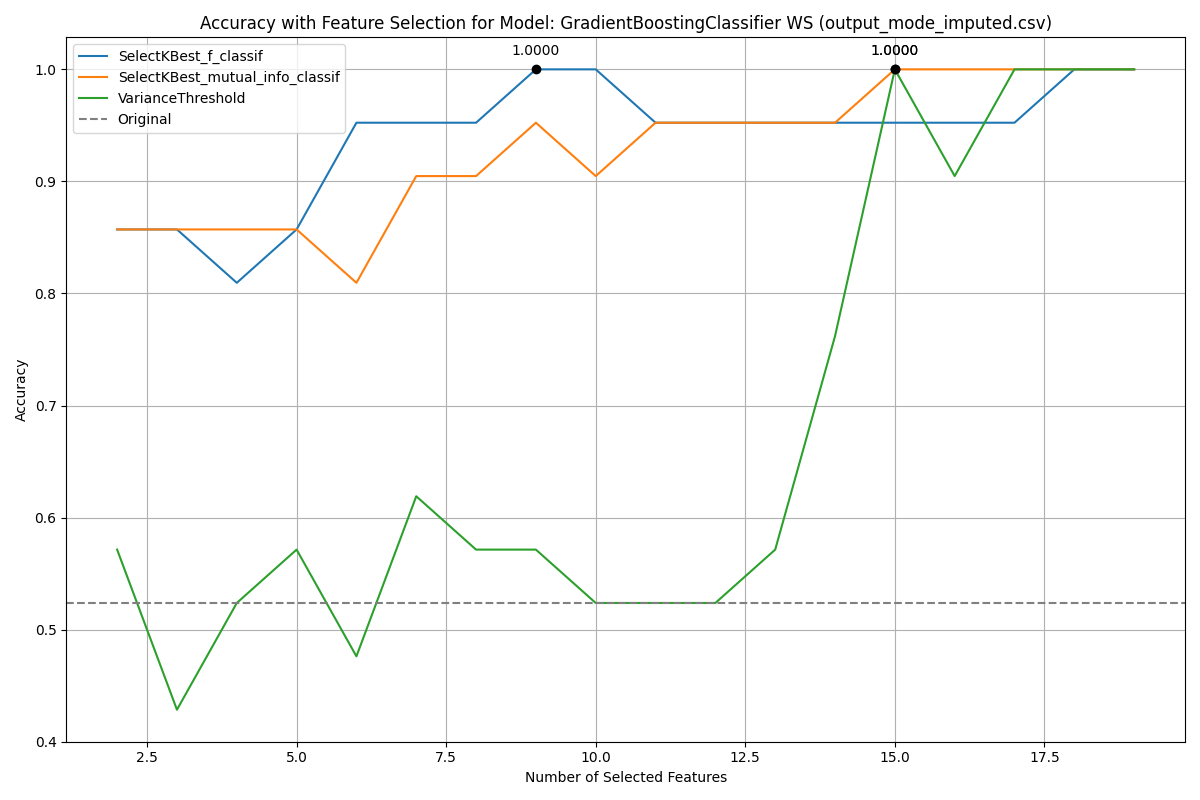
\includegraphics[width=\textwidth]{class_specific_section/images_class_ensemble_reduction/feature_selection_accuracy_plot_output_mode_imputedcsv_GradientBoostingClassifier_WS.png}
        \caption{WS}
        \label{fig_class_spec:ws_featred_graph}
    \end{minipage}
\end{figure}

\begin{figure}[H]
    \centering
    \begin{minipage}[b]{0.45\textwidth}
        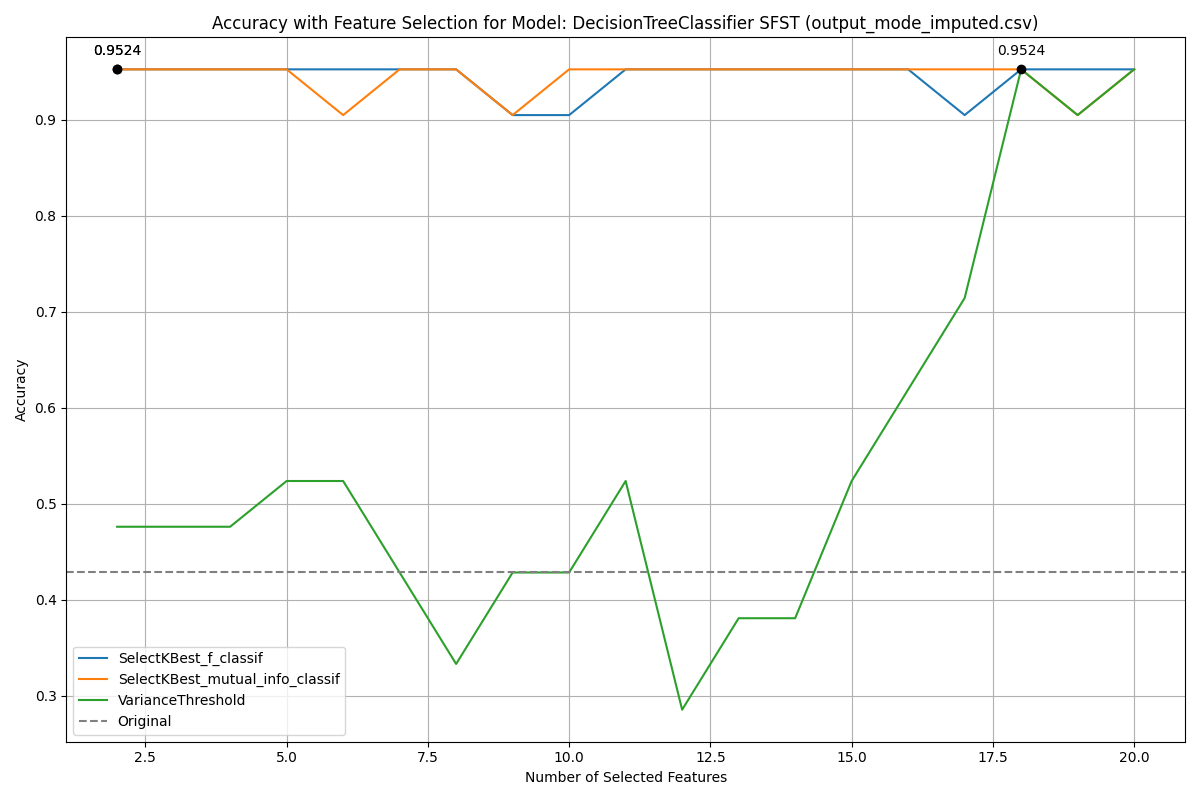
\includegraphics[width=\textwidth]{class_specific_section/images_class_ensemble_reduction/feature_selection_accuracy_plot_output_mode_imputedcsv_DecisionTreeClassifier_SFST.png}
        \caption{SFST}
        \label{fig_class_spec:sfst_featred_graph}
    \end{minipage}
    \hfill
    \begin{minipage}[b]{0.45\textwidth}
        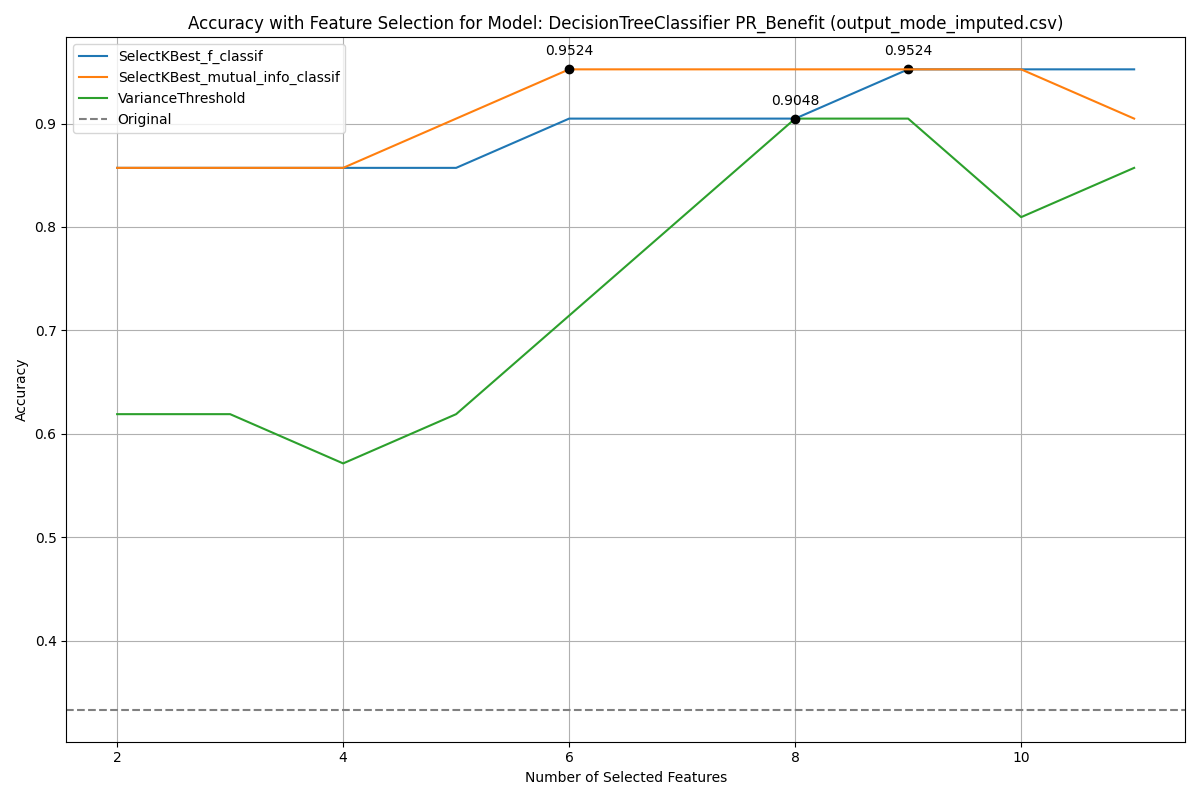
\includegraphics[width=\textwidth]{class_specific_section/images_class_ensemble_reduction/feature_selection_accuracy_plot_output_mode_imputedcsv_DecisionTreeClassifier_PR_Benefit.png}
        \caption{PR Benefit}
        \label{fig_class_spec:pr_ben_featred_graph}
    \end{minipage}
\end{figure}

\begin{figure}[H]
    \centering
    \begin{minipage}[b]{0.45\textwidth}
        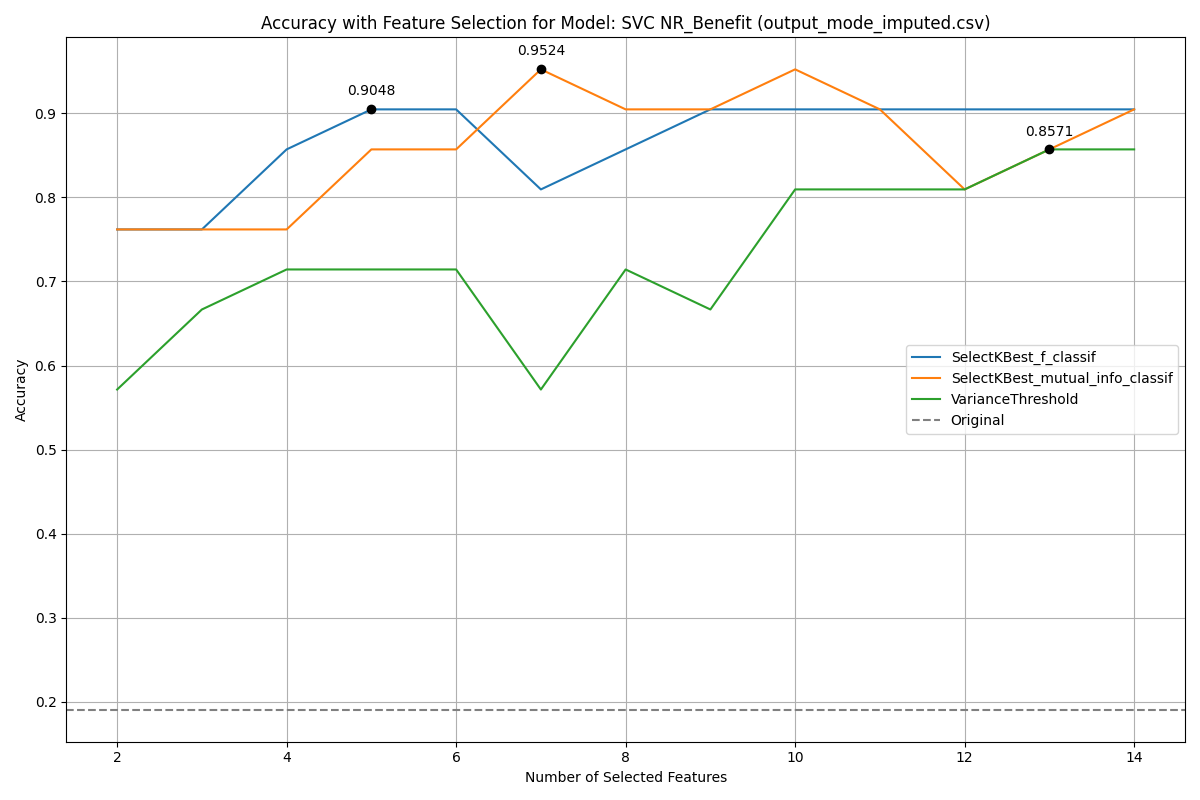
\includegraphics[width=\textwidth]{class_specific_section/images_class_ensemble_reduction/feature_selection_accuracy_plot_output_mode_imputedcsv_SVC_NR_Benefit.png}
        \caption{NR Benefit}
        \label{fig_class_spec:nr_ben_featred_graph}
    \end{minipage}
    \hfill
    \begin{minipage}[b]{0.45\textwidth}
        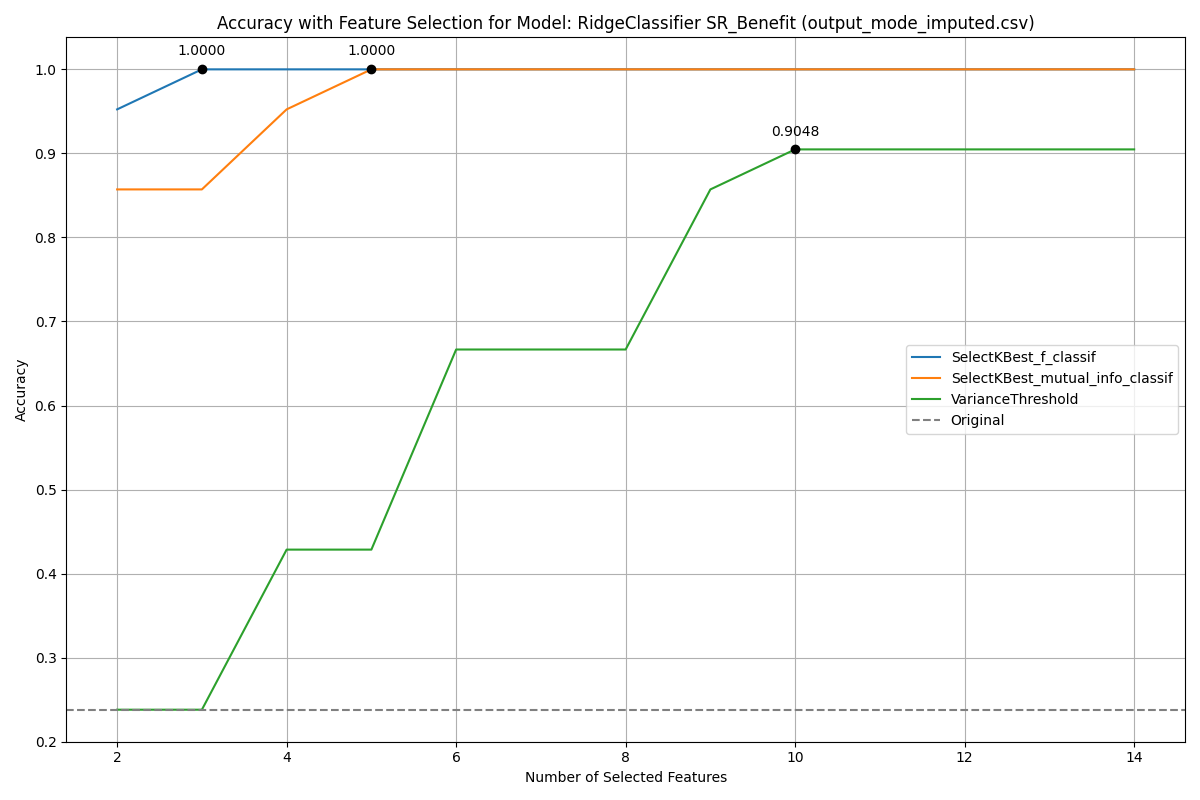
\includegraphics[width=\textwidth]{class_specific_section/images_class_ensemble_reduction/feature_selection_accuracy_plot_output_mode_imputedcsv_RidgeClassifier_SR_Benefit.png}
        \caption{SR Benefit}
        \label{fig_class_spec:sr_ben_featred_graph}
    \end{minipage}
\end{figure}

\begin{figure}[H]
    \centering
    \begin{minipage}[b]{0.45\textwidth}
        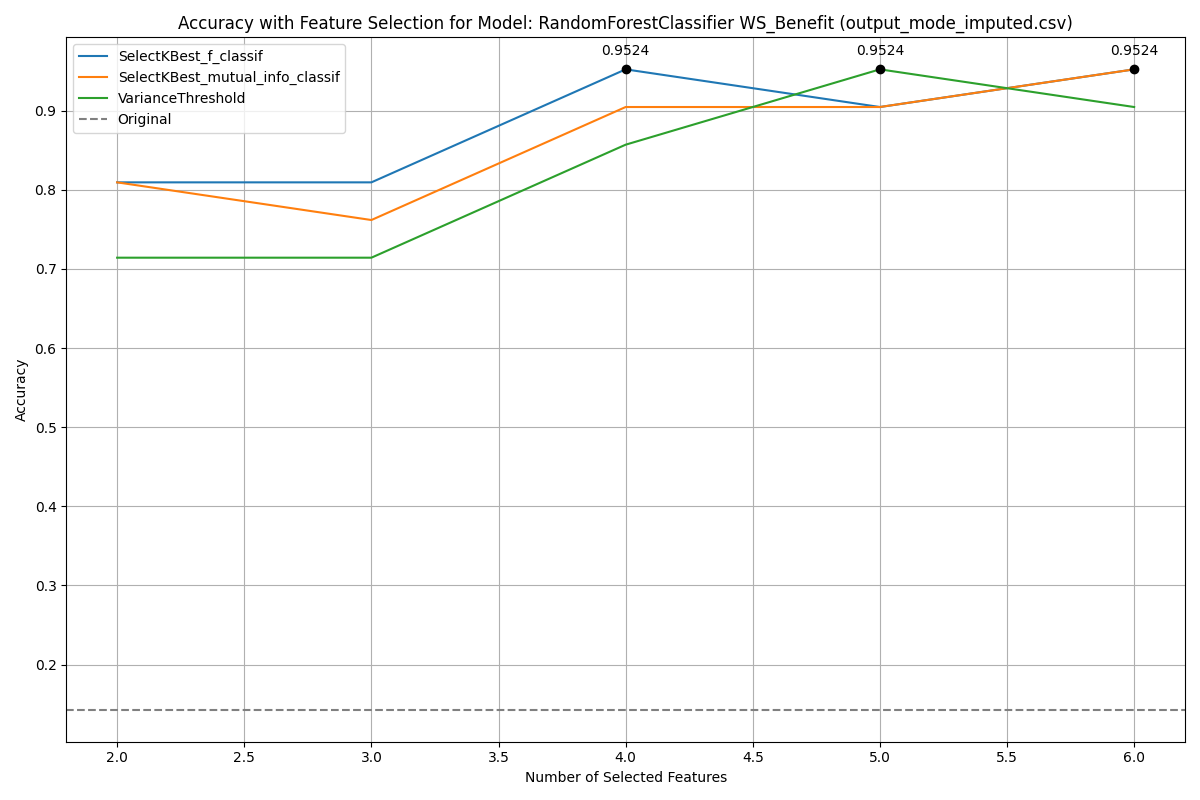
\includegraphics[width=\textwidth]{class_specific_section/images_class_ensemble_reduction/feature_selection_accuracy_plot_output_mode_imputedcsv_RandomForestClassifier_WS_Benefit.png}
        \caption{WS Benefit}
        \label{fig_class_spec:ws_ben_featred_graph}
    \end{minipage}
    \hfill
    \begin{minipage}[b]{0.45\textwidth}
        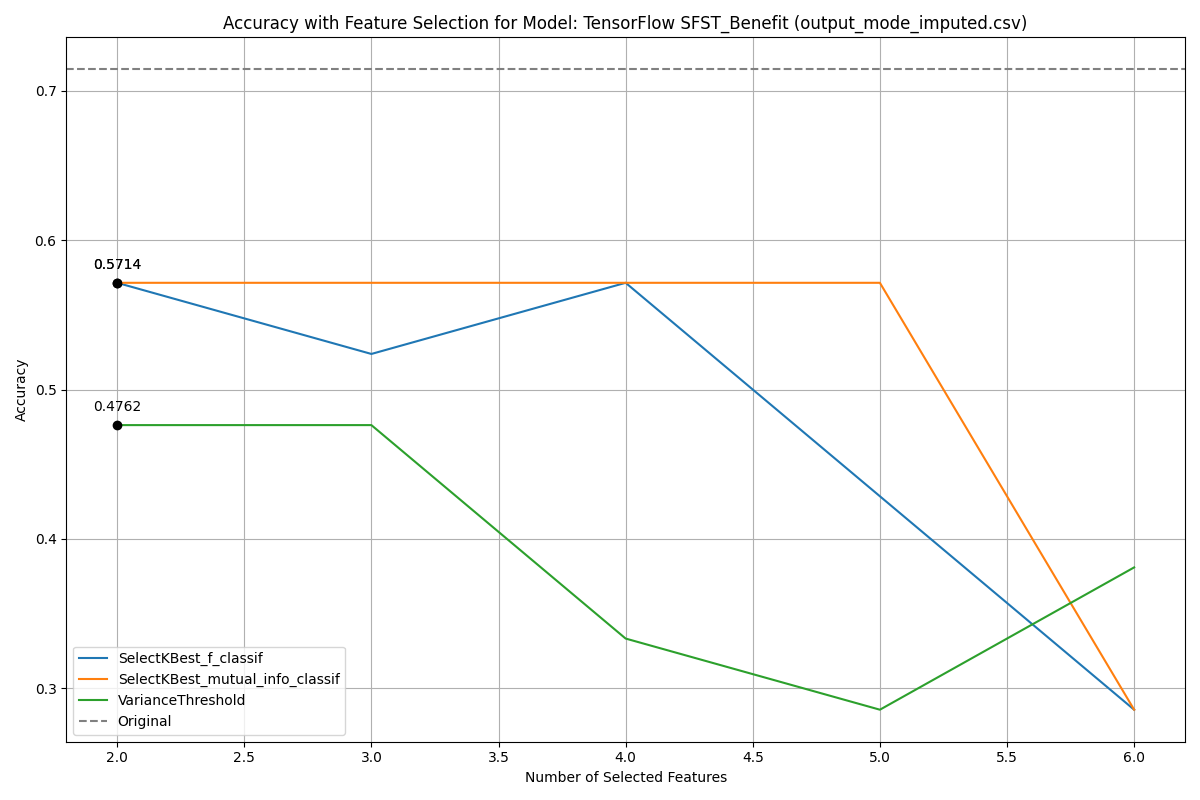
\includegraphics[width=\textwidth]{class_specific_section/images_class_ensemble_reduction/feature_selection_accuracy_plot_output_mode_imputedcsv_TensorFlow_SFST_Benefit.png}
        \caption{SFST Benefit}
        \label{fig_class_spec:sfst_ben_featred_graph}
    \end{minipage}
\end{figure}




\clearpage
\subsection{Regression Models}\label{sec:reg}
\subsubsection{All Features}
\begin{table}
\centering
\begin{tabular}{|c||c|p{4cm}||c|p{4cm}|}
\hline
\multirow{2}{*}{\textbf{Feature}} & \multicolumn{2}{c||}{\textbf{Non-Norm Ensemble}} & \multicolumn{2}{c|}{\textbf{Norm Ensemble}} \\
\cline{2-5}
 & \textbf{MSE} & \textbf{Features Used} & \textbf{MSE} & \textbf{Features Used} \\
\hline
WS & 0.3814 & F22, F23, F24, F28, F30, F31, F43, F44, F46 & 0.3096 & F22, F24, F28, F30, F31, F43, F44, F46 \\
\hline
PR & 0.1893 & F1, F43, F44, F45, F46, Federal Class & 0.1499 & F1, F43, F44, F45, F46, Provincial Class \\
\hline
NR & 0.3131 & F12, F24, F39, F43, F44, F45, F5, F53, Living Moss Depth, OF18, OF27, OF30, Organic Depth & 0.2412 & F12, F24, F43, F44, F45, OF18, OF30, Provincial Class \\
\hline
SR & 1.4574 & F24, F28, F29, F31, F43, F44, F45, F46 & 0.5920 & F24, F28, F29, F31, F43, F44, F45, F46, Provincial Class \\
\hline
SFST & 0.2768 & F30, F43, F44, F45, F46, Provincial Class & 0.2686 & F1, F30, F43, F44, F45, F46, Provincial Class \\
\hline
WS Benefit & 1.2050 & F5, F51, OF17, OF18, OF23, OF24, OF27, Organic Depth & 1.4064 & F12, F53, Hydrogeomorphic Class, OF17, OF18, OF23, OF24, OF30 \\
\hline
PR Benefit & 1.2832 & F14, F31, F3 c, F41, F43, F44, F47, Hydrogeomorphic Class, OF19 & 1.4041 & F14, F41, F43, F47, OF19 \\
\hline
NR Benefit & 3.1188 & F14, F41, F43, Federal Class, OF10, OF19, OF22, OF9, Provincial Class & 3.0601 & F14, F41, F65, Federal Class, OF10, OF19, OF22, OF9, Provincial Class \\
\hline
SR Benefit & 6.8108 & F12, F31, F41, F43, F5, OF18, OF27, OF30 & 3.9488 & F12, F31, F3 c, F41, F43, OF18 \\
\hline
SFST Benefit & 2.1118 & F12, F14, F39, F43, F44, F45, F46, F53, OF18, OF30 & 1.1588 & F1, F31, F43, F44, F45, F46, OF18, S4, S5 \\
\hline
\end{tabular}
\caption{Ensemble Learning MSE and Features Used for Non-Normalized and Normalized Data}
\label{reg_all_tab:summary_mse_features}
\end{table}
%\begin{table}[H]
\centering
\begin{tabular}{|c|c|c|c|c|}
\hline
\textbf{Feature} & \textbf{NNorm MSE} & \textbf{Norm MSE} & \textbf{Model} & \textbf{Dataset} \\
\hline
NR & 0.17 & 0.48 & AdaBoostRegressor & Interpolated \\
\hline
PR & 0.12 & 0.19 & AdaBoostRegressor & custom \\
\hline
SR & 0.37 & 0.62 & AdaBoostRegressor & bfill \\
\hline
SFST & 0.20 & 0.33 & AdaBoostRegressor & ffill \\
\hline
WS & 0.25 & 0.49 & AdaBoostRegressor & knn \\
\hline
NR Benefit & 0.39 & 0.45 & MLPRegressor & ffill \\
\hline
PR Benefit & 0.22 & 0.23 & SGDRegressor & iterative \\
\hline
SR Benefit & 0.17 & 0.22 & AdaBoostRegressor & bfill \\
\hline
SFST Benefit & 0.51 & 0.98 & AdaBoostRegressor & custom \\
\hline
WS Benefit & 1.19 & 1.21 & AdaBoostRegressor & bfill \\
\hline
\end{tabular}
\caption{Best MSE for Non-Normalized and Normalized Data with Algorithm and Dataset}
\label{reg_all_tab:norm_mse}
\end{table}


\begin{table}[H]
\centering
\begin{tabular}{|c|c|c|c|}
\hline
\textbf{Feature} & \textbf{PNorm MSE} & \textbf{Model} & \textbf{Dataset}  \\
\hline
NR & 0.31& AdaBoostRegressor & knn  \\
\hline
PR  & 0.21 & AdaBoostRegressor & iterative\\
\hline
SR & 0.46 & AdaBoostRegressor & knn \\
\hline
SFST & 0.26& AdaBoostRegressor & custom  \\
\hline
WS & 0.60 & AdaBoostRegressor & custom \\
\hline
NR Benefit & 0.28& MLPRegressor & knn  \\
\hline
PR Benefit  & 0.49 \& MLPRegressor & ffill \\
\hline
SR Benefit & 0.07& SGDRegressor & mode  \\
\hline
SFST Benefit & 0.71& AdaBoostRegressor & iterative  \\
\hline
WS Benefit & 0.63& AdaBoostRegressor & mean  \\
\hline
\end{tabular}
\caption{Best MSE for Pre-Normalized Data}
\label{reg_all_tab:pre_norm_mse}
\end{table}

%\begin{figure}[H]
    \centering
    \begin{minipage}{0.45\textwidth}
        \centering
        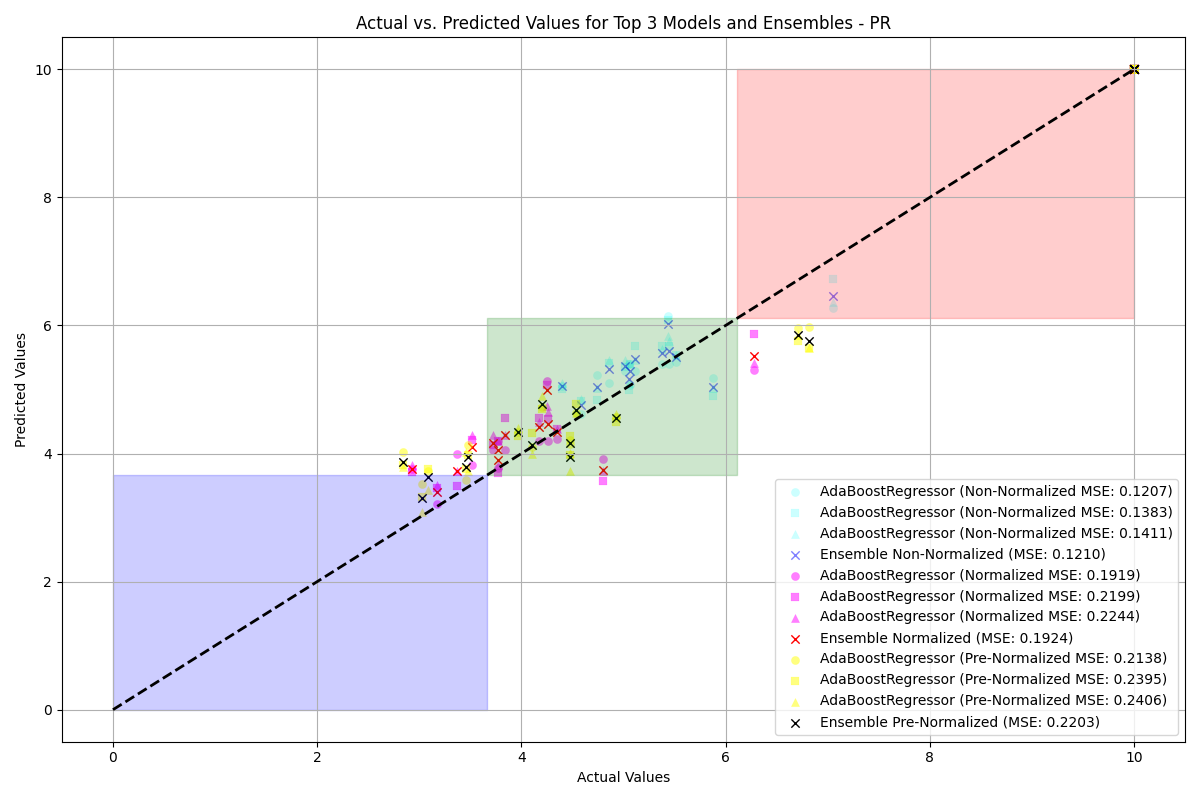
\includegraphics[width=\linewidth]{reg_section_all/ensemble_learning/actual_vs_predicted_top_3_models_and_ensembles_PR.png}
        \caption{PR}
        \label{reg_all_fig:pr_ensemble}
    \end{minipage}\hfill
    \begin{minipage}{0.45\textwidth}
        \centering
        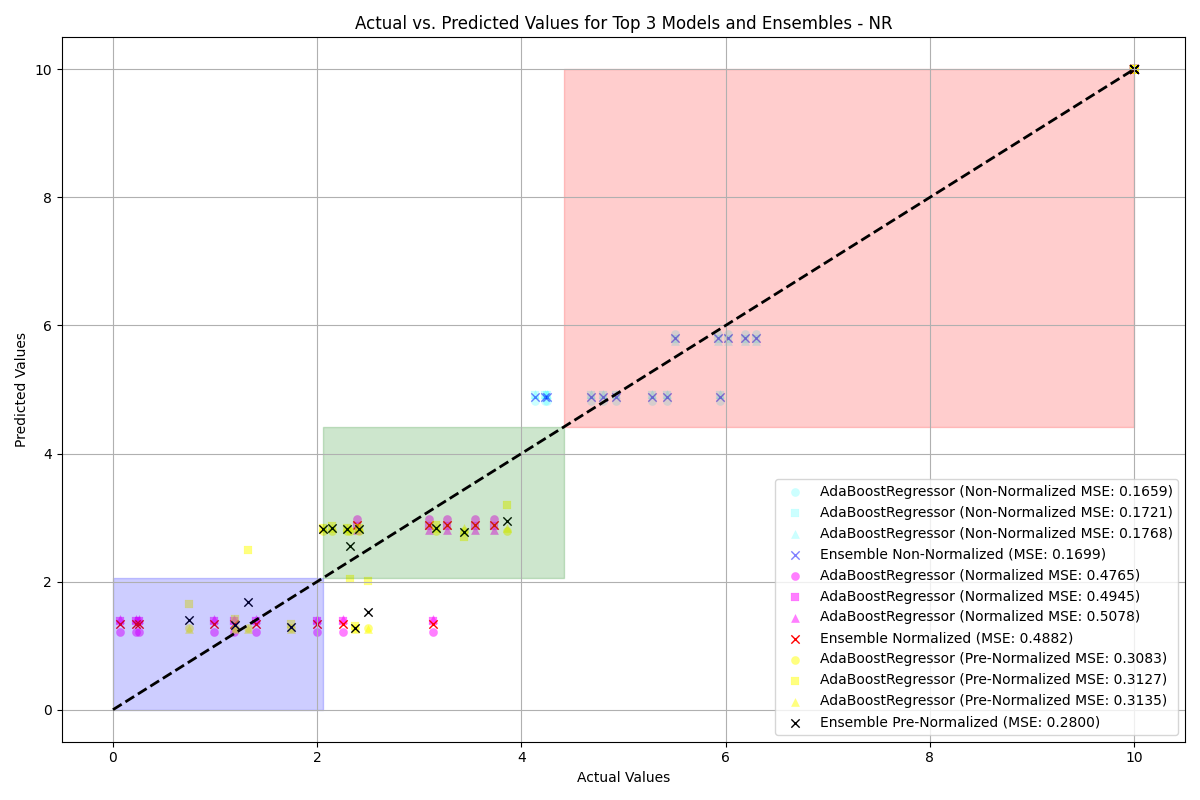
\includegraphics[width=\linewidth]{reg_section_all/ensemble_learning/actual_vs_predicted_top_3_models_and_ensembles_NR.png}
        \caption{NR}
        \label{reg_all_fig:nr_ensemble}
    \end{minipage}
\end{figure}

\begin{figure}[H]
    \centering
    \begin{minipage}{0.45\textwidth}
        \centering
        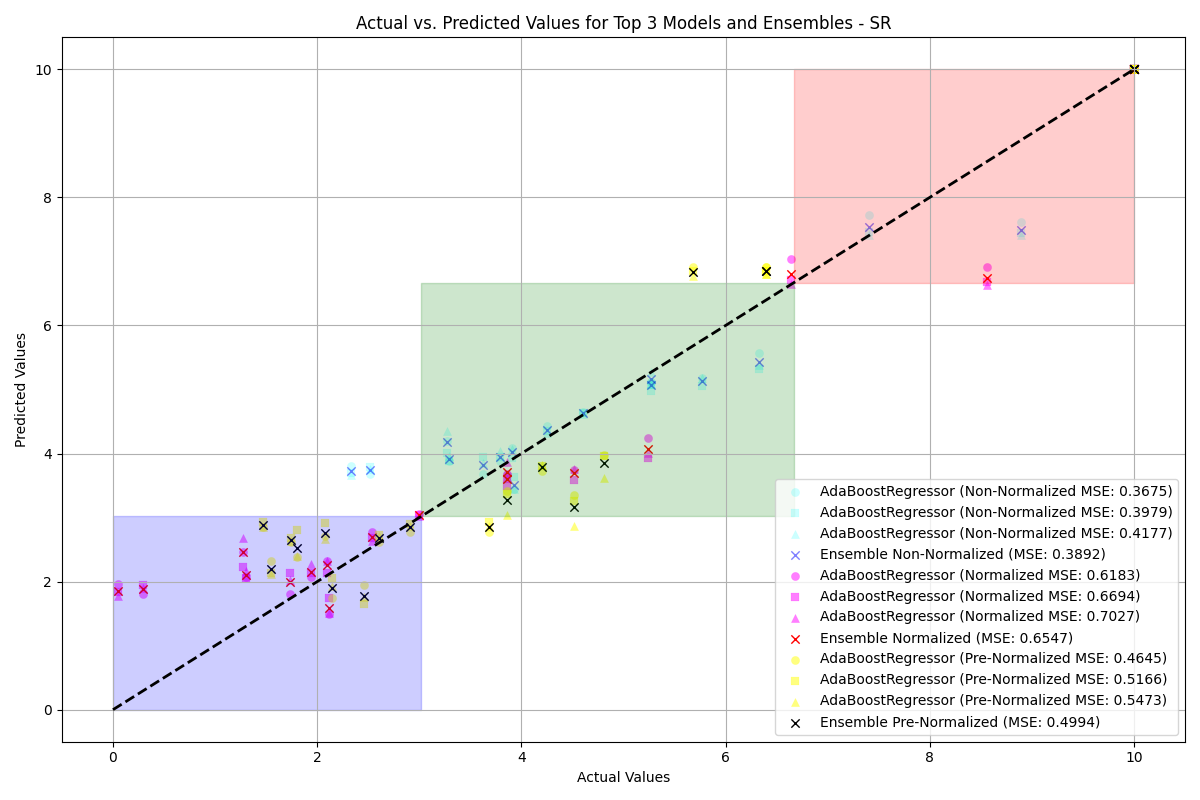
\includegraphics[width=\linewidth]{reg_section_all/ensemble_learning/actual_vs_predicted_top_3_models_and_ensembles_SR.png}
        \caption{SR}
        \label{reg_all_fig:sr_ensemble}
    \end{minipage}\hfill
    \begin{minipage}{0.45\textwidth}
        \centering
        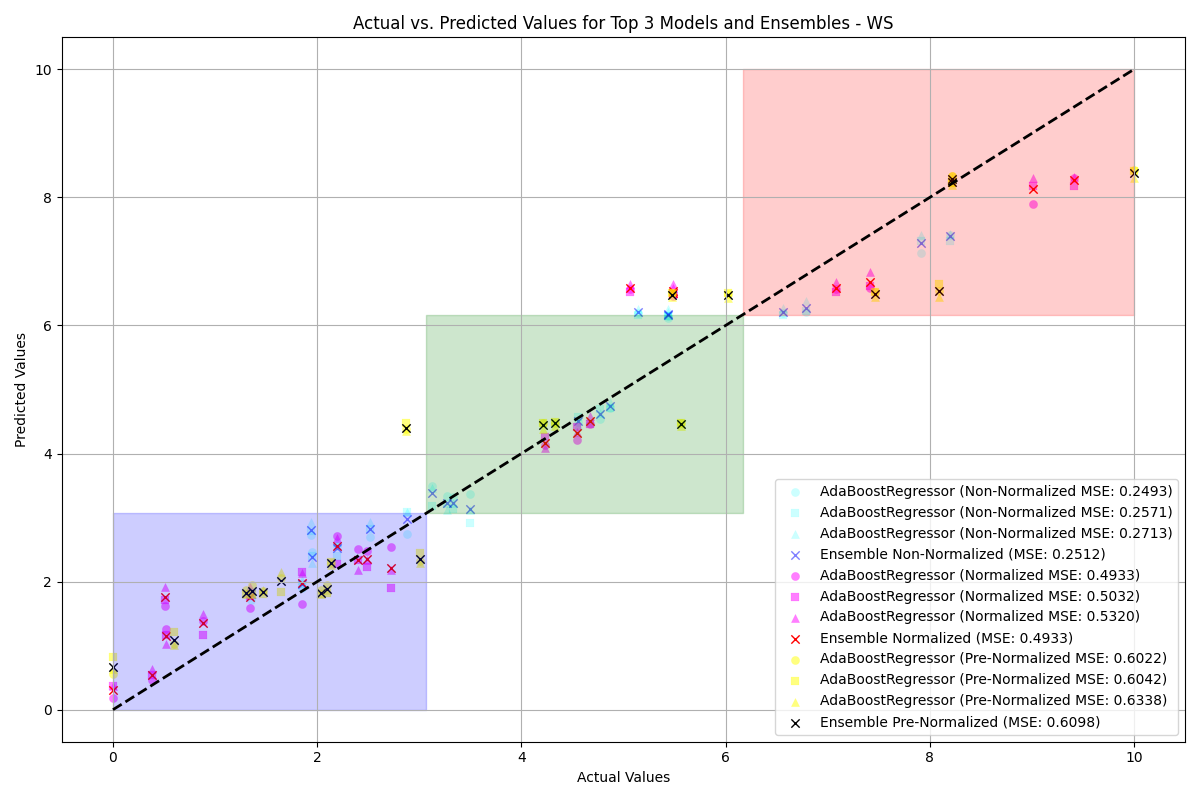
\includegraphics[width=\linewidth]{reg_section_all/ensemble_learning/actual_vs_predicted_top_3_models_and_ensembles_WS.png}
        \caption{WS}
        \label{reg_all_fig:ws_ensemble}
    \end{minipage}
\end{figure}

\begin{figure}[H]
    \centering
    \begin{minipage}{0.45\textwidth}
        \centering
        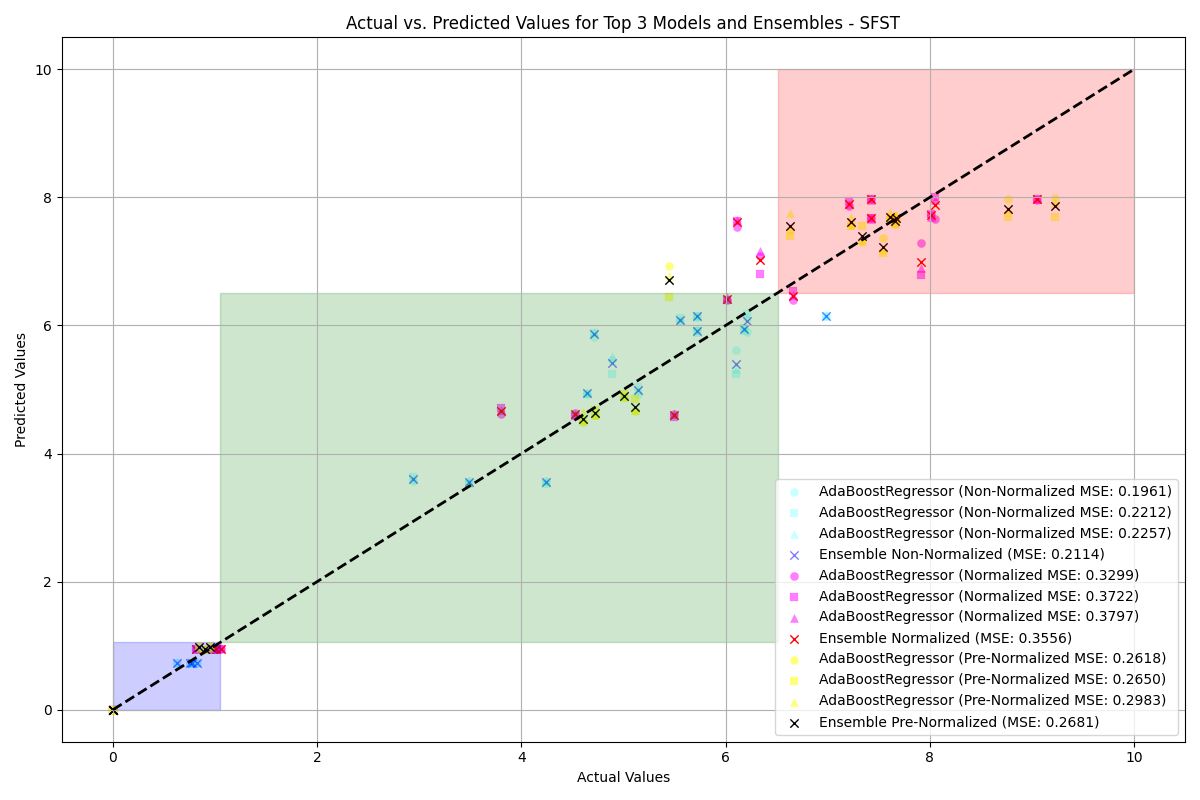
\includegraphics[width=\linewidth]{reg_section_all/ensemble_learning/actual_vs_predicted_top_3_models_and_ensembles_SFST.png}
        \caption{SFST}
        \label{reg_all_fig:sfst_ensemble}
    \end{minipage}\hfill
    \begin{minipage}{0.45\textwidth}
        \centering
        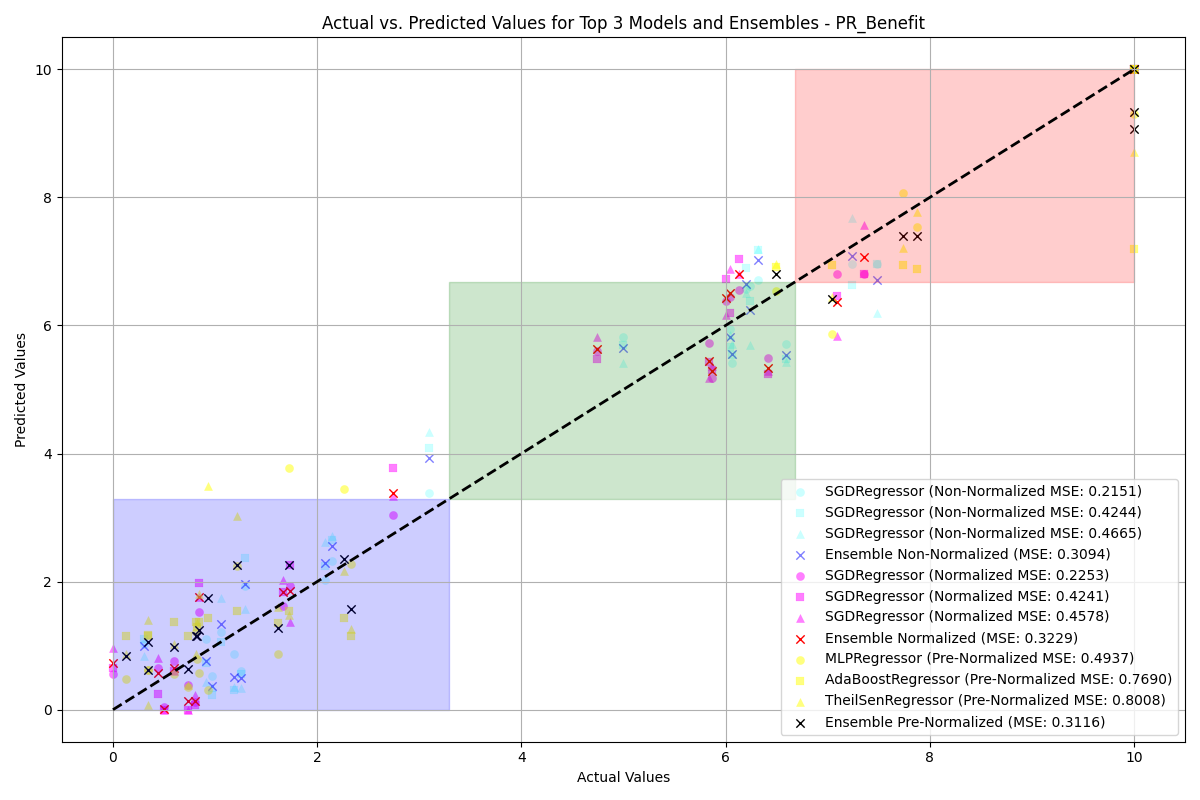
\includegraphics[width=\linewidth]{reg_section_all/ensemble_learning/actual_vs_predicted_top_3_models_and_ensembles_PR_Benefit.png}
        \caption{PR Benefit}
        \label{reg_all_fig:pr_ben_ensemble}
    \end{minipage}
\end{figure}

\begin{figure}[H]
    \centering
    \begin{minipage}{0.45\textwidth}
        \centering
        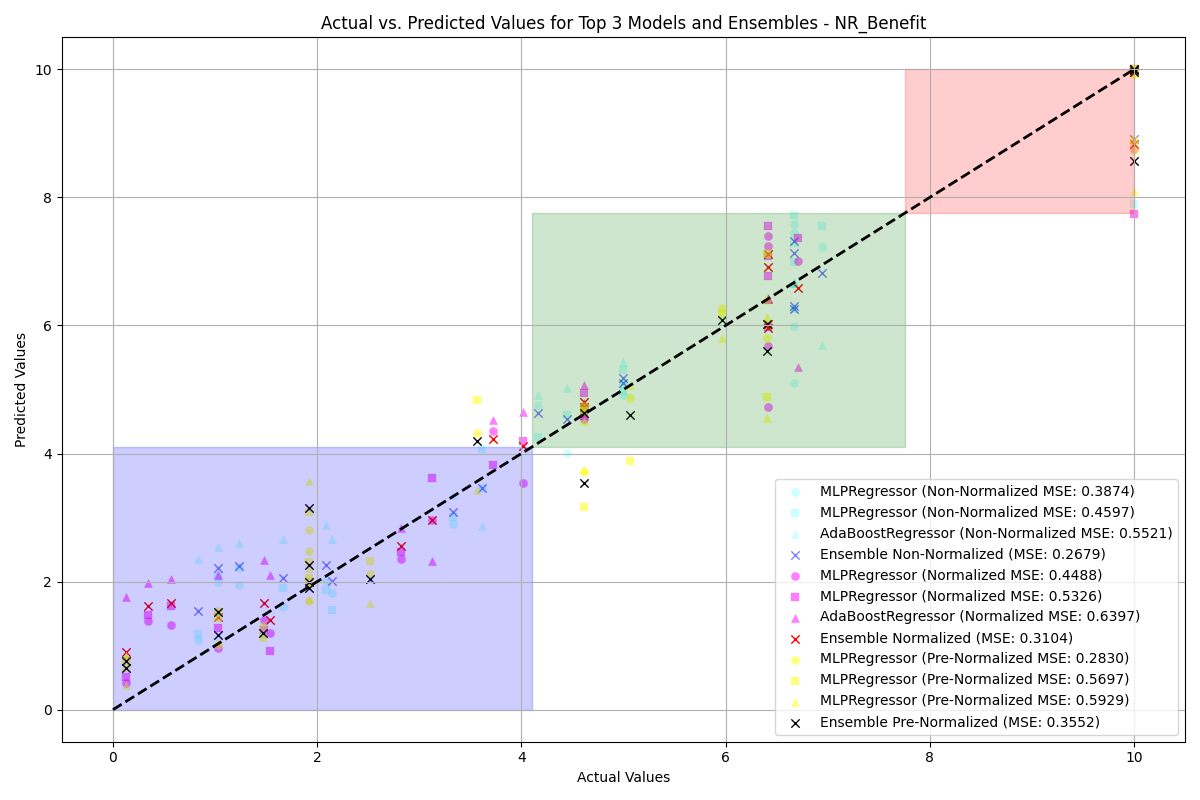
\includegraphics[width=\linewidth]{reg_section_all/ensemble_learning/actual_vs_predicted_top_3_models_and_ensembles_NR_Benefit.png}
        \caption{NR Benefit}
        \label{reg_all_fig:nr_ben_ensemble}
    \end{minipage}\hfill
    \begin{minipage}{0.45\textwidth}
        \centering
        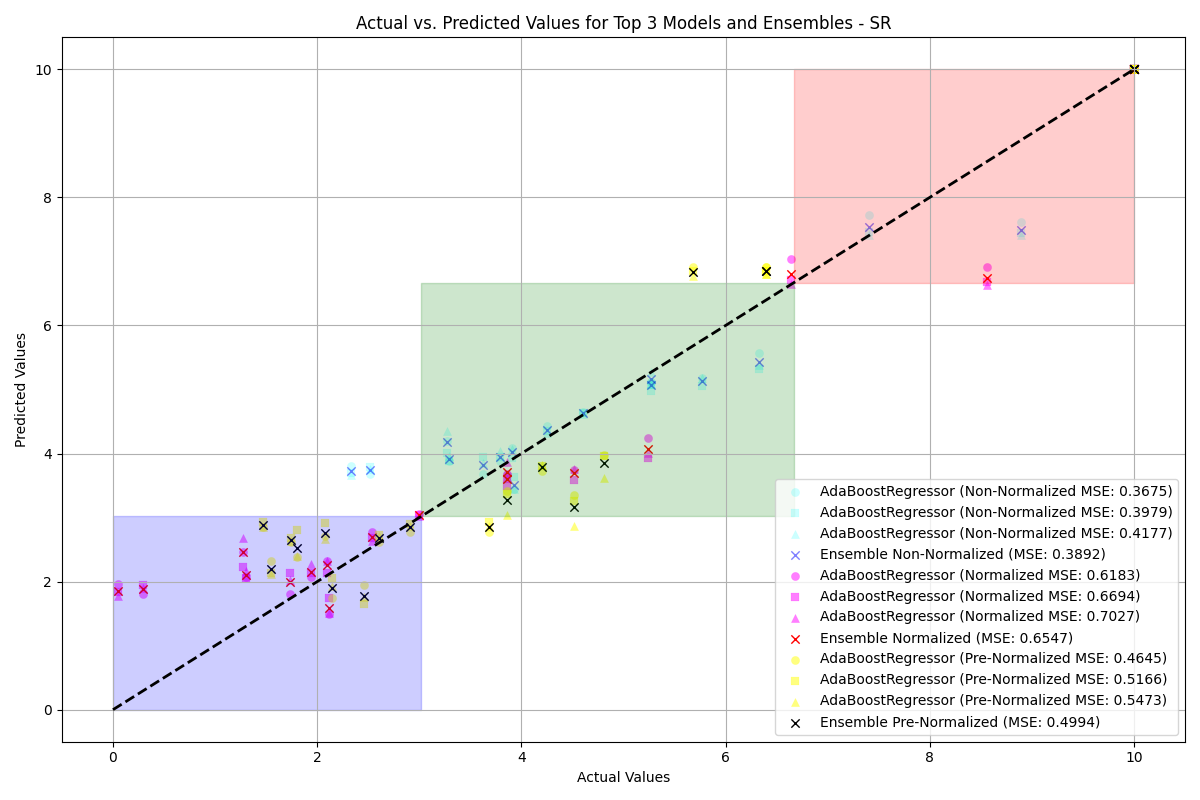
\includegraphics[width=\linewidth]{reg_section_all/ensemble_learning/actual_vs_predicted_top_3_models_and_ensembles_SR.png}
        \caption{SR Benefit}
        \label{reg_all_fig:sr_ben_ensemble}
    \end{minipage}
\end{figure}

\begin{figure}[H]
    \centering
    \begin{minipage}{0.45\textwidth}
        \centering
        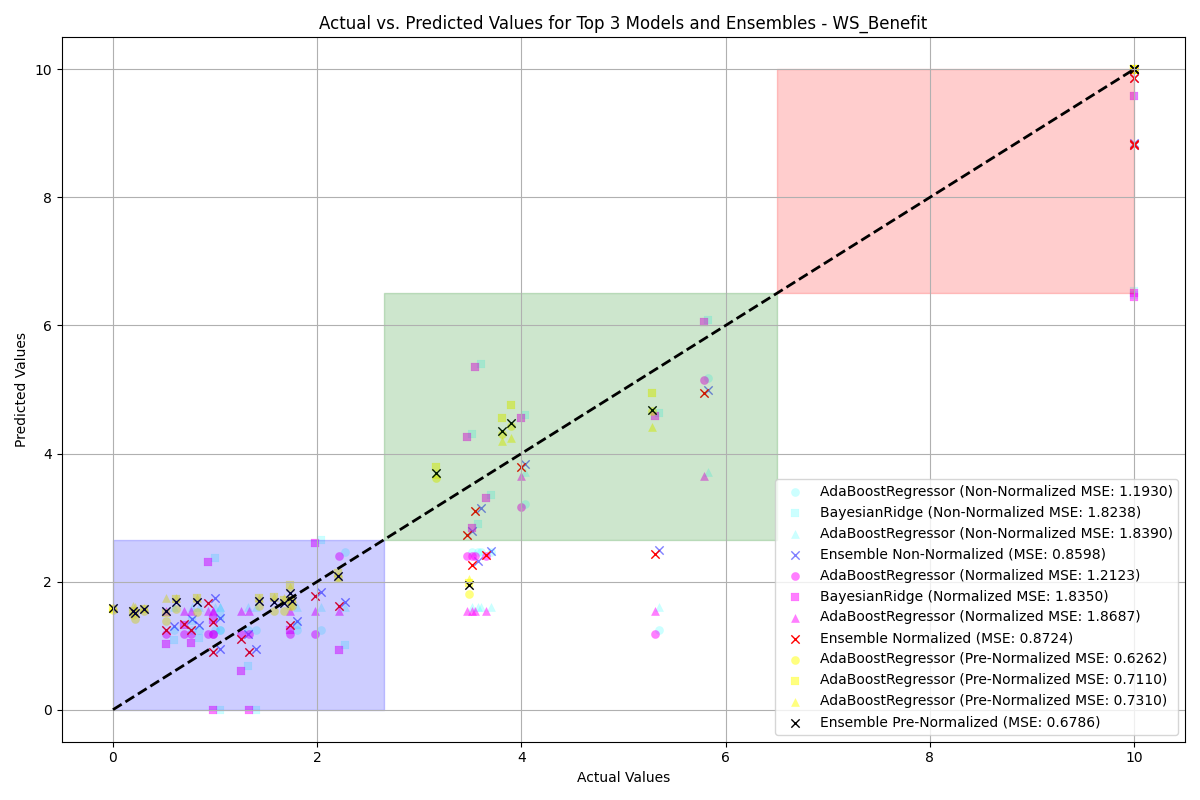
\includegraphics[width=\linewidth]{reg_section_all/ensemble_learning/actual_vs_predicted_top_3_models_and_ensembles_WS_Benefit.png}
        \caption{WS Benefit}
        \label{reg_all_fig:ws_ben_ensemble}
    \end{minipage}\hfill
    \begin{minipage}{0.45\textwidth}
        \centering
        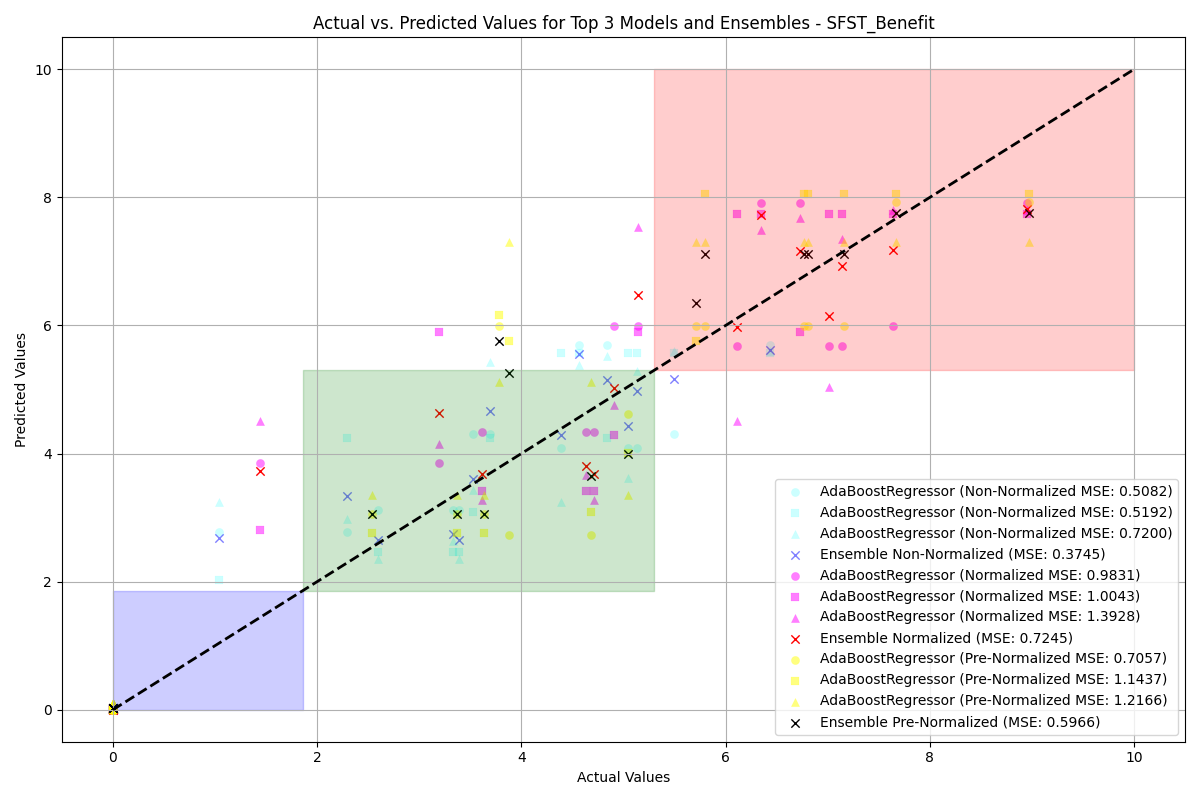
\includegraphics[width=\linewidth]{reg_section_all/ensemble_learning/actual_vs_predicted_top_3_models_and_ensembles_SFST_Benefit.png}
        \caption{SFST Benefit}
        \label{reg_all_fig:sfst_ben_ensemble}
    \end{minipage}
\end{figure}

%\begin{longtable}{|p{2cm}|p{2cm}|p{2cm}|p{2cm}|p{2cm}|p{4cm}|}
\hline
\textbf{Model} & \textbf{Lower Acc.} & \textbf{Moderate Acc.} & \textbf{Higher Acc.} & \textbf{Overall Acc.} & \textbf{Top Features} \\ \hline
\endfirsthead
\hline
\textbf{Model} & \textbf{Lower Acc.} & \textbf{Moderate Acc.} & \textbf{Higher Acc.} & \textbf{Overall Acc.} & \textbf{Top Features} \\ \hline
\endhead

WS & 80.81\% & 64.20\% & 70.37\% & 74.07\% & Provincial\_Class, Hydrogeomorphic\_Class, OF22, F22, F28, F31, F43, F44, F45 \\ \hline
PR & 13.89\% & 77.78\% & 87.50\% & 69.31\% & Provincial\_Class, Federal\_Class, F43, F44, F45 \\ \hline
NR & 32.80\% & 65.08\% & 76.19\% & 58.02\% & Provincial\_Class, F24, F43, F44, F45 \\ \hline
SR & 62.22\% & 60.00\% & 62.35\% & 61.73\% & F28, F29, F31, F44, F45 \\ \hline
SFST & 56.17\% & 60.85\% & 76.39\% & 65.43\% & F1, F43 \\ \hline
WS Benefit & 68.35\% & 46.56\% & 44.44\% & 57.67\% & Hydrogeomorphic\_Class, OF17, OF18, OF23, OF24, F51 \\ \hline
PR Benefit & 80.00\% & 44.97\% & 29.63\% & 58.73\% & Regime, Moss\_Cover, Living\_Moss\_Depth, OF19, OF20, OF21, OF22, OF24, F41 \\ \hline
NR Benefit & 70.74\% & 80.42\% & 49.07\% & 69.84\% & Living\_Moss\_Depth, OF9, OF10, OF19, OF20, OF21, OF22, OF23, F41 \\ \hline
SR Benefit & 93.70\% & 53.91\% & 0.00\% & 67.72\% & Provincial\_Class, Federal\_Class, Regime, Vegetation\_Type, Living\_Moss\_Depth, Organic\_Depth, Hydrogeomorphic\_Class, OF18, OF24, F41 \\ \hline
SFST Benefit & 59.72\% & 32.10\% & 48.15\% & 47.97\% & Provincial\_Class, Federal\_Class, Moss\_Cover, Surface\_Water\_Present, Hydrogeomorphic\_Class, OF18, OF22, OF25, OF28 \\ \hline
\caption{Classification Accuracies and Top Features for Various Models}
\label{tab:grouping_1d}
\end{longtable}

\begin{longtable}{|p{1.5cm}|p{2.0cm}|p{2.0cm}|p{2.0cm}|p{2.0cm}|p{4cm}|}
\hline
\textbf{Model} & \textbf{Lower Acc.} & \textbf{Moderate Acc.} & \textbf{Higher Acc.} & \textbf{Overall Acc.} & \textbf{Top Features} \\ \hline
\endfirsthead
\hline
\textbf{Model} & \textbf{Lower Acc.} & \textbf{Moderate Acc.} & \textbf{Higher Acc.} & \textbf{Overall Acc.} & \textbf{Top Features} \\ \hline
\endhead

WS & 100.00\% & 50.00\% & 100.00\% & 85.71\% & F22, F31, F43, F44, F46, F5, OF18, OF27 \\ \hline
PR & 0.00\% & 100.00\% & 100.00\% & 76.19\% & F43, F44, F45, F5, OF18, OF27 \\ \hline
NR & 0.00\% & 71.43\% & 42.86\% & 80.95\% & F43, F44, F45, F5, OF18, OF27, OF34, S4 \\ \hline
SR & 30.00\% & 80.00\% & 50.00\% & 90.48\% & F24, F28, F31, F43, F44, F45, F5, OF18, OF27 \\ \hline
SFST & 100.00\% & 42.86\% & 100.00\% & 80.95\% & F43, F44, F45, F46, OF18, OF27 \\ \hline
WS Benefit & 54.55\% & 71.43\% & 66.67\% & 90.48\% & F5, OF17, OF18, OF23, OF27, OF34, S4 \\ \hline
PR Benefit & 100.00\% & 85.71\% & 25.00\% & 80.95\% & F14, F3\_c, F41, F44, OF18, OF19, OF27 \\ \hline
NR Benefit & 100.00\% & 85.71\% & 50.00\% & 85.71\% & F41, F5, OF10, OF18, OF19, OF22, OF27, OF9 \\ \hline
SR Benefit & 100.00\% & 0.00\% & 0.00\% & 85.71\% & F12, F41, OF18, OF22, OF27, OF30 \\ \hline
SFST Benefit & 37.50\% & 100.00\% & 42.86\% & 80.95\% & F12, F43, F44, F45, F5, OF18, OF27, OF30 \\ \hline
\caption{Ensemble Model Accuracies}
\label{tab:grouping_2d}
\end{longtable}

\begin{longtable}{|p{1.5cm}|p{2.0cm}|p{2.0cm}|p{2.0cm}|p{2.0cm}|p{4cm}|}
\hline
\textbf{Model} & \textbf{Lower Acc.} & \textbf{Moderate Acc.} & \textbf{Higher Acc.} & \textbf{Overall Acc.} & \textbf{Top Features} \\ \hline
\endfirsthead
\hline
\textbf{Model} & \textbf{Lower Acc.} & \textbf{Moderate Acc.} & \textbf{Higher Acc.} & \textbf{Overall Acc.} & \textbf{Top Features} \\ \hline
\endhead

WS & 100.00\% & 50.00\% & 75.00\% & 85.71\% & F22, F31, F43, F44, F46, F5, OF18, OF27 \\ \hline
PR & 0.00\% & 100.00\% & 100.00\% & 76.19\% & F43, F44, F45, F5, OF18, OF27 \\ \hline
NR & 0.00\% & 85.71\% & 42.86\% & 61.90\% & F43, F44, F45, F5, OF18, OF27, OF34, S4 \\ \hline
SR & 30.00\% & 80.00\% & 33.33\% & 85.71\% & F24, F28, F31, F43, F44, F45, F5, OF18, OF27 \\ \hline
SFST & 100.00\% & 42.86\% & 100.00\% & 80.95\% & F43, F44, F45, F46, OF18, OF27 \\ \hline
WS Benefit & 36.36\% & 71.43\% & 66.67\% & 80.95\% & F5, OF17, OF18, OF23, OF27, OF34, S4 \\ \hline
PR Benefit & 100.00\% & 85.71\% & 25.00\% & 80.95\% & F14, F3\_c, F41, F44, OF18, OF19, OF27 \\ \hline
NR Benefit & 100.00\% & 85.71\% & 50.00\% & 76.19\% & F41, F5, OF10, OF18, OF19, OF22, OF27, OF9 \\ \hline
SR Benefit & 100.00\% & 0.00\% & 0.00\% & 47.62\% & F12, F41, OF18, OF22, OF27, OF30 \\ \hline
SFST Benefit & 37.50\% & 100.00\% & 42.86\% & 57.14\% & F12, F43, F44, F45, F5, OF18, OF27, OF30 \\ \hline

\caption{Voting System Accuracies}
\label{tab:grouping_3d}
\end{longtable}

%\begin{figure}[H]
    \centering
    \begin{minipage}{0.45\textwidth}
        \centering
        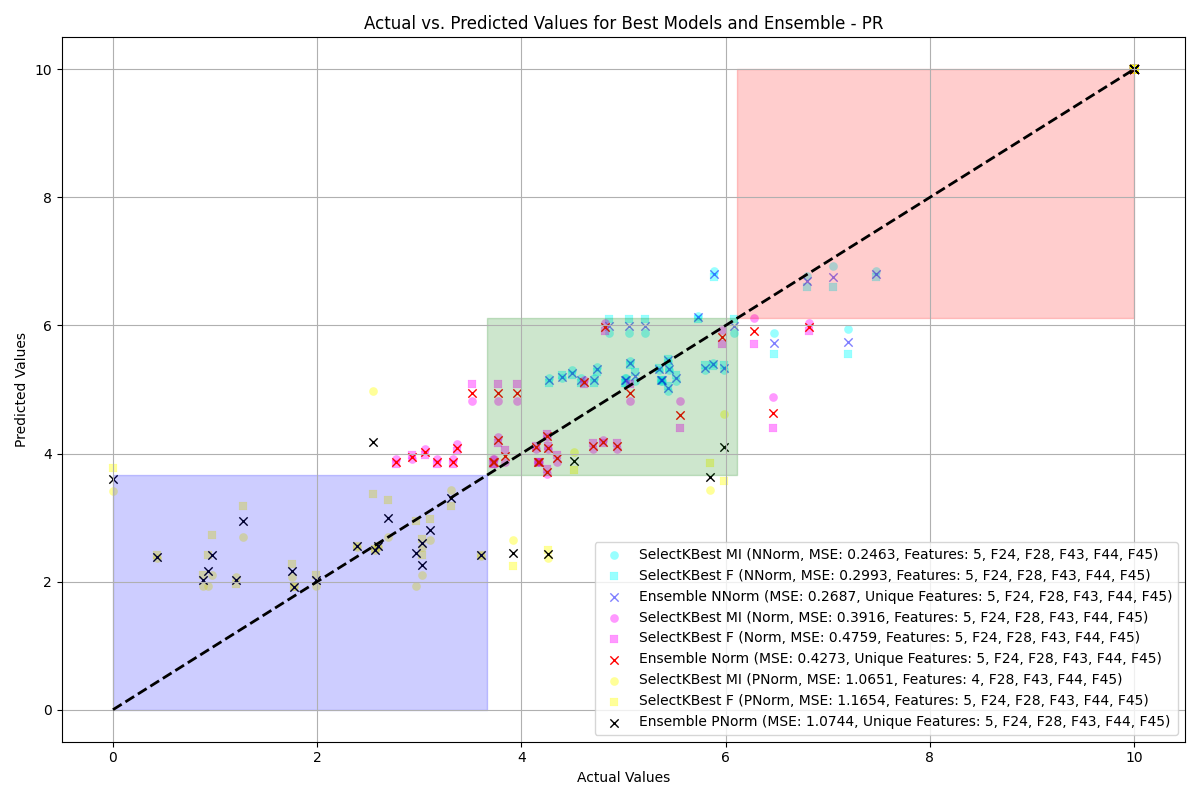
\includegraphics[width=\linewidth]{reg_section_specific/featred_ensemble_learning/actual_vs_predicted_best_feature_selection_and_ensemble_PR_10.png}
        \caption{PR}
        \label{reg_spec_fig:pr_featred}
    \end{minipage}\hfill
    \begin{minipage}{0.45\textwidth}
        \centering
        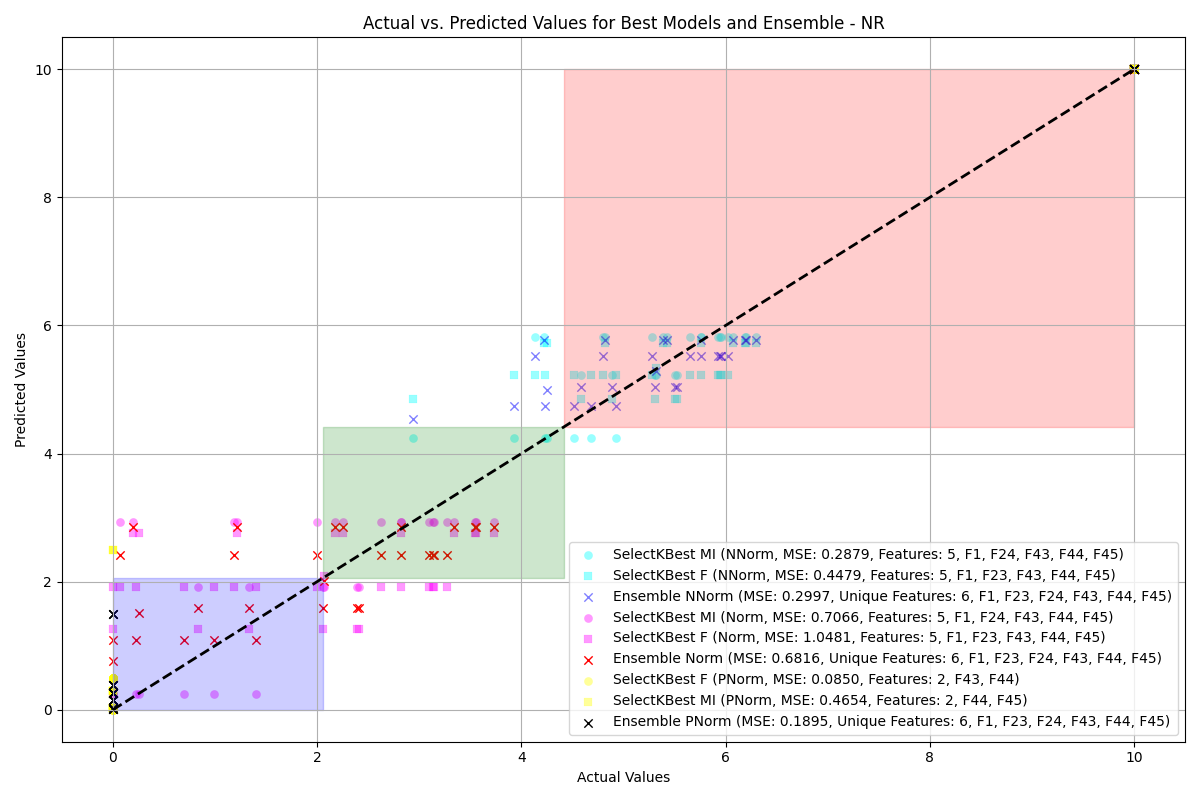
\includegraphics[width=\linewidth]{reg_section_specific/featred_ensemble_learning/actual_vs_predicted_best_feature_selection_and_ensemble_NR_10.png}
        \caption{NR}
        \label{reg_spec_fig:nr_featred}
    \end{minipage}
\end{figure}

\begin{figure}[H]
    \centering
    \begin{minipage}{0.45\textwidth}
        \centering
        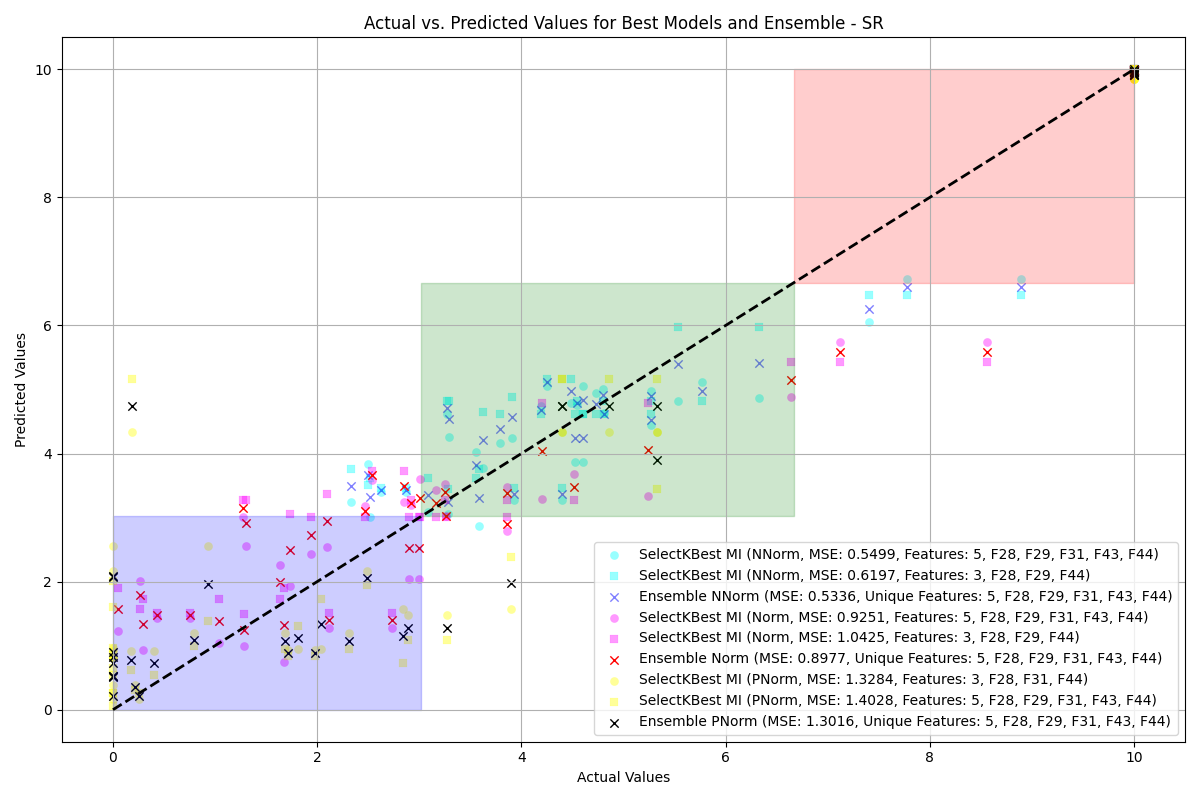
\includegraphics[width=\linewidth]{reg_section_specific/featred_ensemble_learning/actual_vs_predicted_best_feature_selection_and_ensemble_SR_10.png}
        \caption{SR}
        \label{reg_spec_fig:sr_featred}
    \end{minipage}\hfill
    \begin{minipage}{0.45\textwidth}
        \centering
        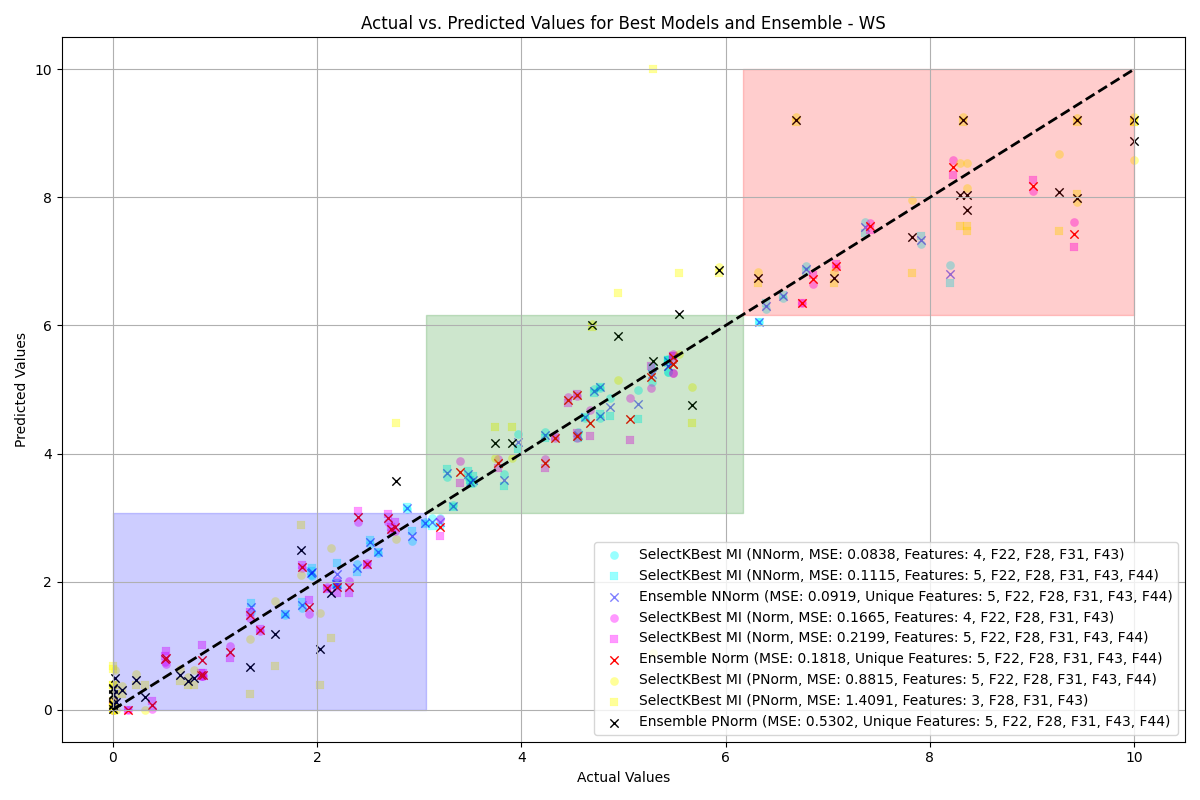
\includegraphics[width=\linewidth]{reg_section_specific/featred_ensemble_learning/actual_vs_predicted_best_feature_selection_and_ensemble_WS_10.png}
        \caption{WS}
        \label{reg_spec_fig:ws_featred}
    \end{minipage}
\end{figure}

\begin{figure}[H]
    \centering
    \begin{minipage}{0.45\textwidth}
        \centering
        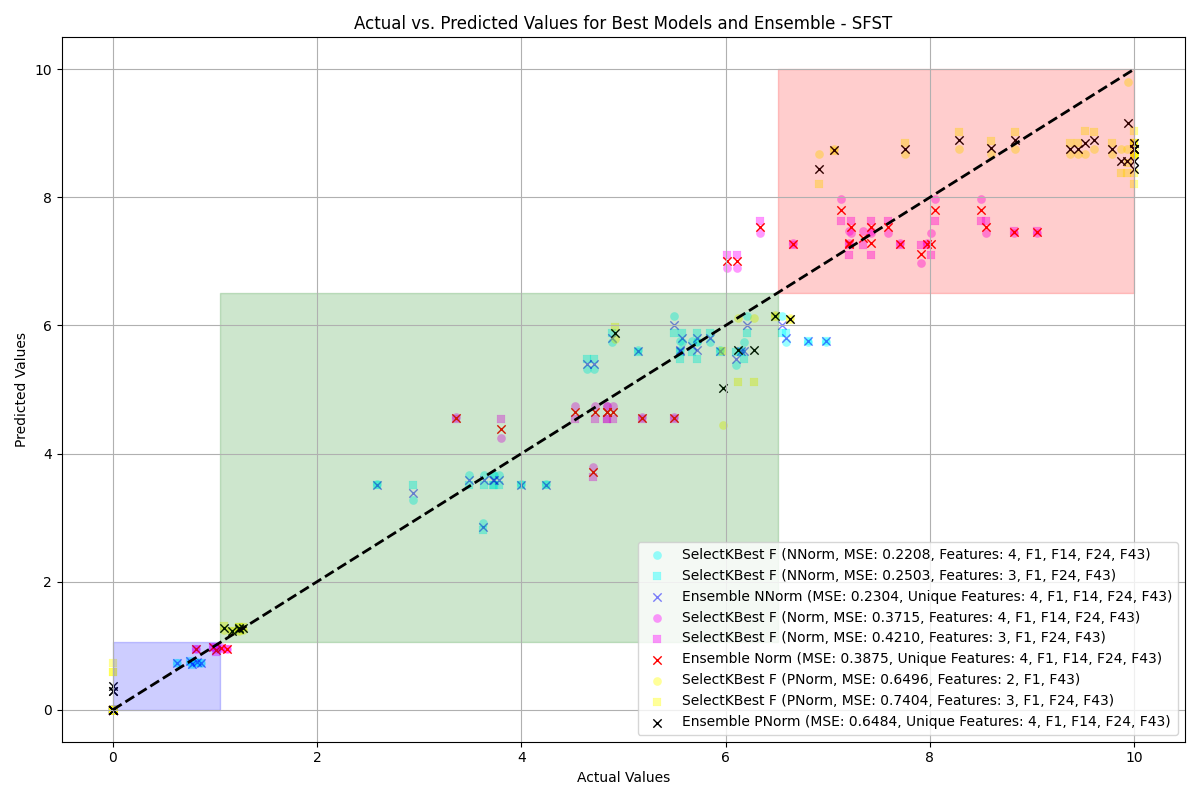
\includegraphics[width=\linewidth]{reg_section_specific/featred_ensemble_learning/actual_vs_predicted_best_feature_selection_and_ensemble_SFST_10.png}
        \caption{SFST}
        \label{reg_spec_fig:sfst_featred}
    \end{minipage}\hfill
    \begin{minipage}{0.45\textwidth}
        \centering
        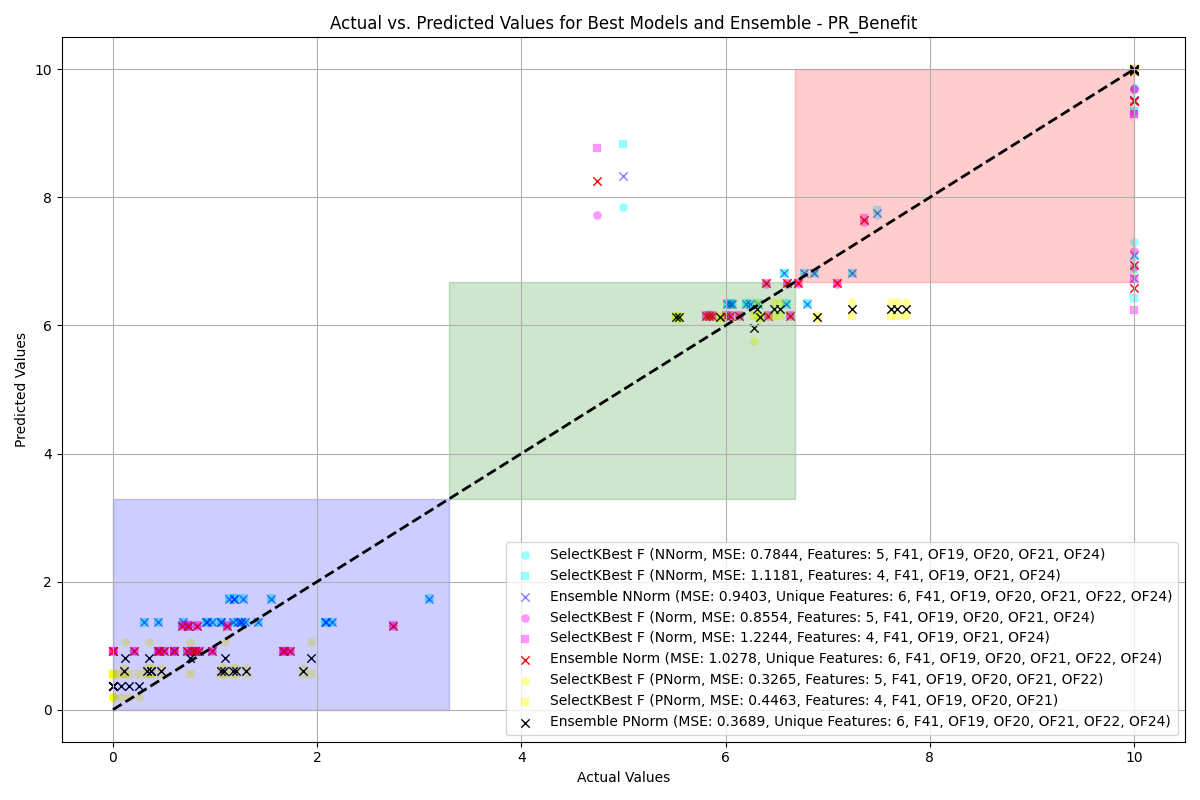
\includegraphics[width=\linewidth]{reg_section_specific/featred_ensemble_learning/actual_vs_predicted_best_feature_selection_and_ensemble_PR_Benefit_10.png}
        \caption{PR Benefit}
        \label{reg_spec_fig:pr_ben_featred}
    \end{minipage}
\end{figure}

\begin{figure}[H]
    \centering
    \begin{minipage}{0.45\textwidth}
        \centering
        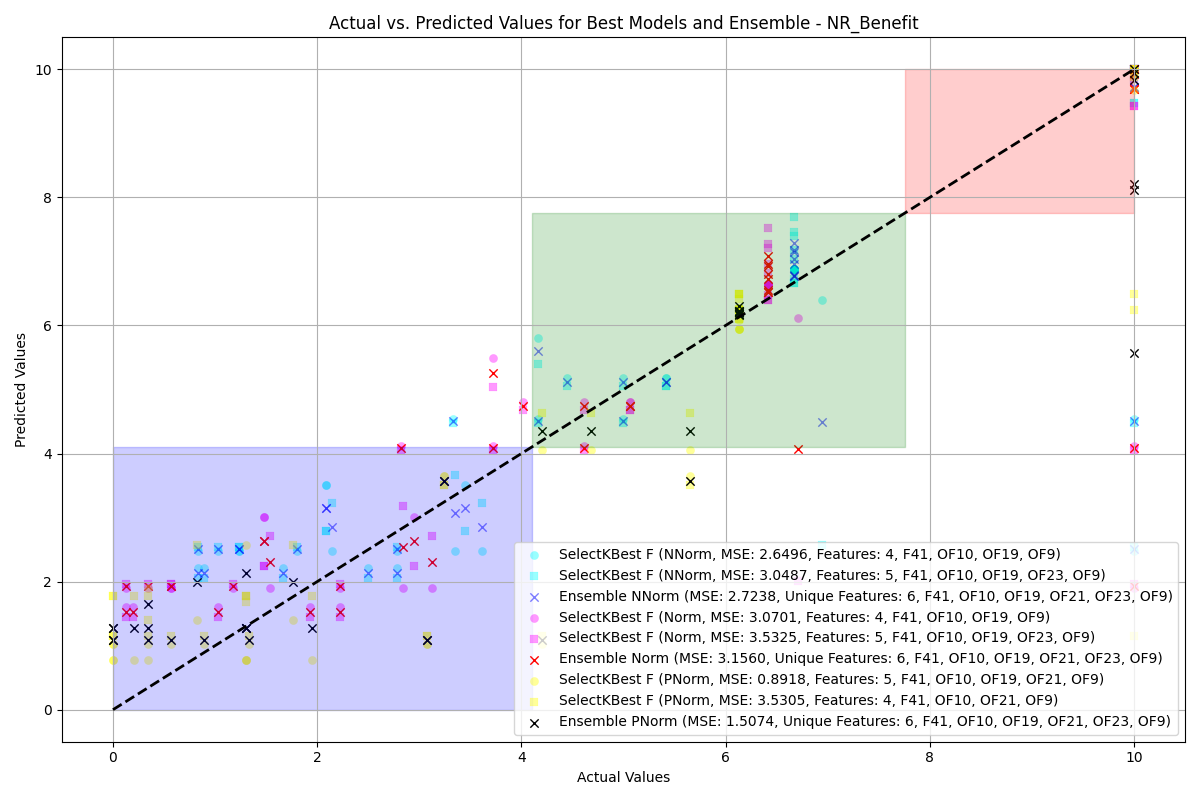
\includegraphics[width=\linewidth]{reg_section_specific/featred_ensemble_learning/actual_vs_predicted_best_feature_selection_and_ensemble_NR_Benefit_10.png}
        \caption{NR Benefit}
        \label{reg_spec_fig:nr_ben_featred}
    \end{minipage}\hfill
    \begin{minipage}{0.45\textwidth}
        \centering
        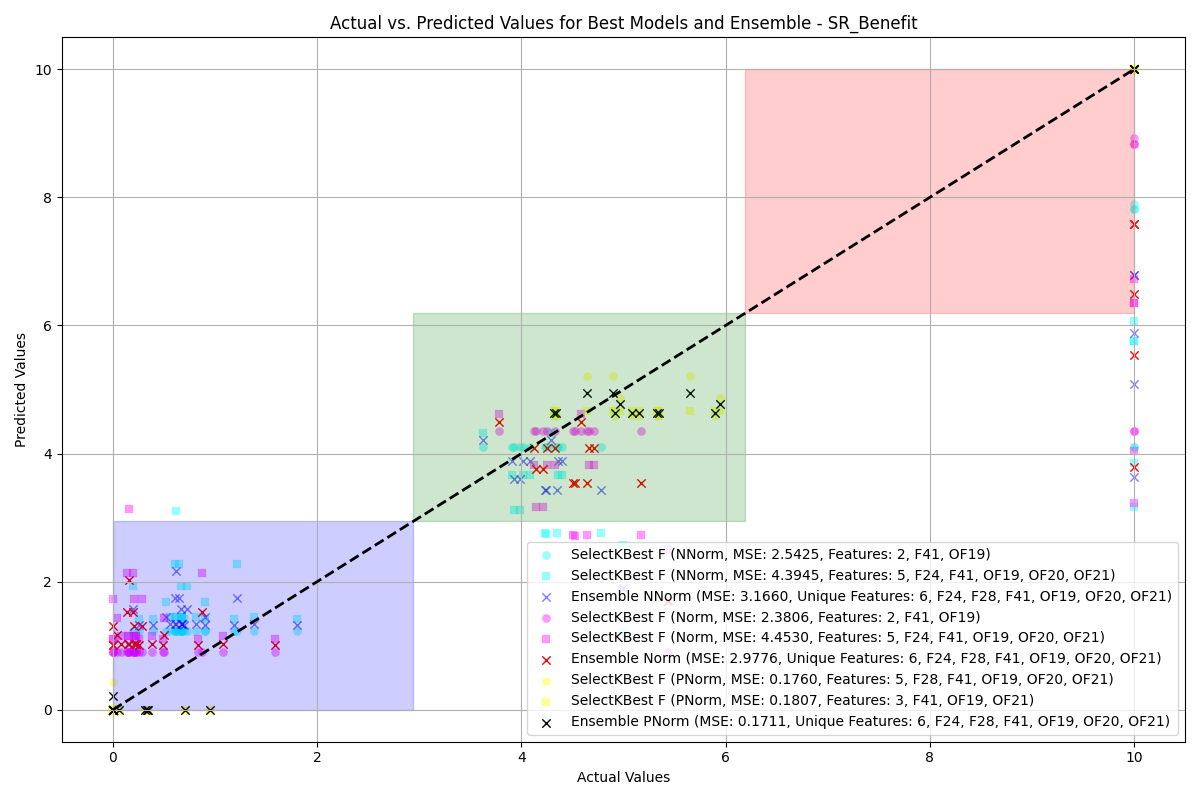
\includegraphics[width=\linewidth]{reg_section_specific/featred_ensemble_learning/actual_vs_predicted_best_feature_selection_and_ensemble_SR_Benefit_10.png}
        \caption{SR Benefit}
        \label{reg_spec_fig:sr_ben_featred}
    \end{minipage}
\end{figure}

\begin{figure}[H]
    \centering
    \begin{minipage}{0.45\textwidth}
        \centering
        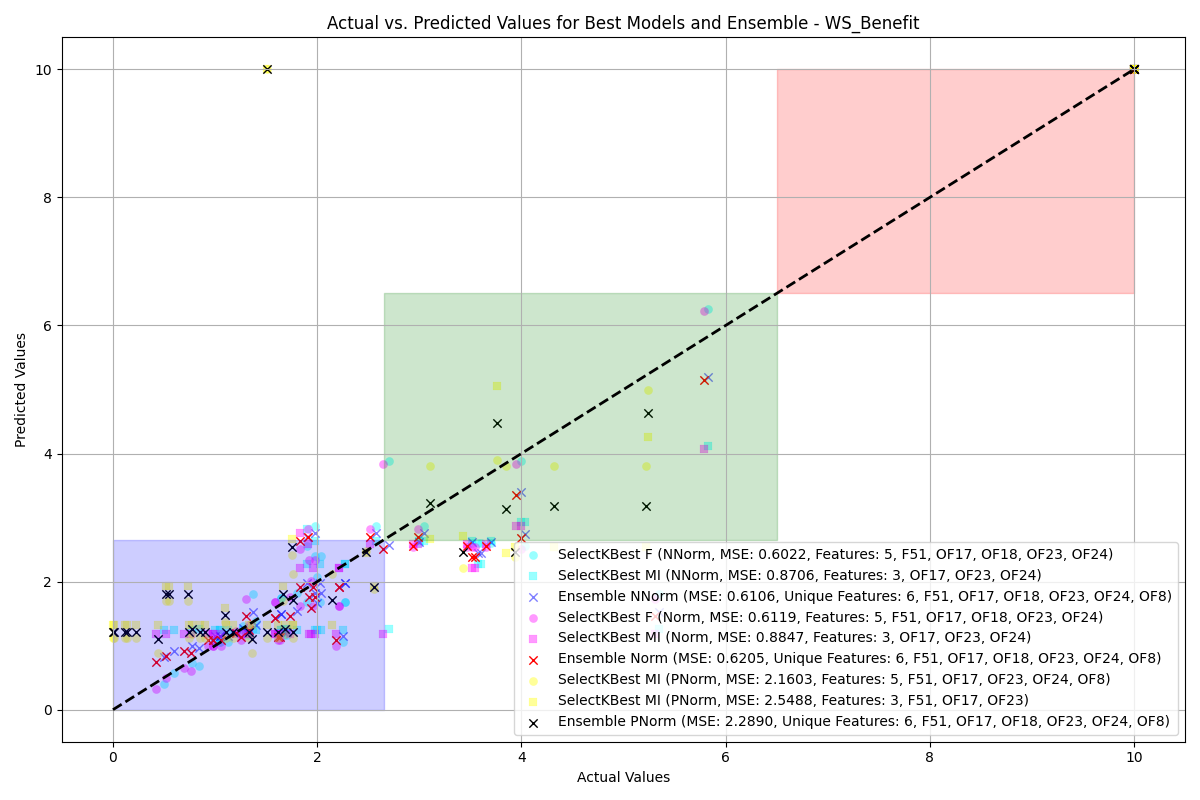
\includegraphics[width=\linewidth]{reg_section_specific/featred_ensemble_learning/actual_vs_predicted_best_feature_selection_and_ensemble_WS_Benefit_10.png}
        \caption{WS Benefit}
        \label{reg_spec_fig:ws_ben_featred}
    \end{minipage}\hfill
    \begin{minipage}{0.45\textwidth}
        \centering
        \includegraphics[width=\linewidth]{reg_section_specific/featred_ensemble_learning/actual_vs_predicted_best_feature_selection_and_ensemble_SFST_Benefit_10.png}
        \caption{SFST Benefit}
        \label{reg_spec_fig:sfst_ben_featred}
    \end{minipage}
\end{figure}

%\begin{table}[H]
\centering
\begin{tabular}{|c|c|c|c|c|c|c|}
\hline
\multirow{2}{*}{\textbf{Function}} & \multicolumn{3}{c|}{\textbf{Top Model}} & \multicolumn{3}{c|}{\textbf{Ensemble}} \\
\cline{2-7}
 & \textbf{Lower} & \textbf{Moderate} & \textbf{Higher} & \textbf{Lower} & \textbf{Moderate} & \textbf{Higher} \\
\hline
WS & 100.00\% & 50.00\% & 100.00\% & 100.00\% & 50.00\% & 100.00\% \\
\hline
PR & 0.00\% & 100.00\% & 87.50\% & 0.00\% & 100.00\% & 87.50\% \\
\hline
NR & 57.14\% & 71.43\% & 100.00\% & 28.57\% & 85.71\% & 100.00\% \\
\hline
SR & 90.00\% & 80.00\% & 83.33\% & 90.00\% & 100.00\% & 83.33\% \\
\hline
SFST & 100.00\% & 42.86\% & 100.00\% & 100.00\% & 42.86\% & 100.00\% \\
\hline
WS\_Benefit & 100.00\% & 28.57\% & 100.00\% & 100.00\% & 28.57\% & 100.00\% \\
\hline
PR\_Benefit & 100.00\% & 42.86\% & 50.00\% & 100.00\% & 85.71\% & 50.00\% \\
\hline
NR\_Benefit & 80.00\% & 100.00\% & 75.00\% & 100.00\% & 100.00\% & 75.00\% \\
\hline
SR\_Benefit & 20.00\% & 88.89\% & 0.00\% & 20.00\% & 88.89\% & 0.00\% \\
\hline
SFST\_Benefit & 87.50\% & 50.00\% & 100.00\% & 87.50\% & 50.00\% & 100.00\% \\
\hline
\end{tabular}
\caption{Comparison of Top Model and Ensemble Accuracy for Non-Normalized Data}
\label{reg_all_tab:featred_non_norm_accuracy}
\end{table}

\begin{table}[H]
\centering
\begin{tabular}{|c|c|c|c|c|c|c|}
\hline
\multirow{2}{*}{\textbf{Function}} & \multicolumn{3}{c|}{\textbf{Top Model}} & \multicolumn{3}{c|}{\textbf{Ensemble}} \\
\cline{2-7}
 & \textbf{Lower} & \textbf{Moderate} & \textbf{Higher} & \textbf{Lower} & \textbf{Moderate} & \textbf{Higher} \\
\hline
WS & 100.00\% & 80.00\% & 100.00\% & 100.00\% & 60.00\% & 100.00\% \\
\hline
PR & N/A & 100.00\% & 100.00\% & N/A & 100.00\% & 87.50\% \\
\hline
NR & N/A & 0.00\% & 100.00\% & N/A & 0.00\% & 100.00\% \\
\hline
SR & 0.00\% & 100.00\% & 71.43\% & 0.00\% & 100.00\% & 100.00\% \\
\hline
SFST & 100.00\% & 100.00\% & 0.00\% & 100.00\% & 100.00\% & 0.00\% \\
\hline
WS\_Benefit & 100.00\% & 28.57\% & 100.00\% & 81.82\% & 42.86\% & 100.00\% \\
\hline
PR\_Benefit & 100.00\% & 85.71\% & 50.00\% & 100.00\% & 57.14\% & 50.00\% \\
\hline
NR\_Benefit & 75.00\% & 77.78\% & 75.00\% & 100.00\% & 77.78\% & 75.00\% \\
\hline
SR\_Benefit & 100.00\% & 88.89\% & 0.00\% & 100.00\% & 88.89\% & 0.00\% \\
\hline
SFST\_Benefit & 87.50\% & 100.00\% & 0.00\% & 87.50\% & 100.00\% & 0.00\% \\
\hline
\end{tabular}
\caption{Comparison of Top Model and Ensemble Accuracy for Pre-Normalized Data}
\label{reg_all_tab:featred_norm_accuracy}
\end{table}



\subsubsection{Specific Features}
\begin{table}[H]
\centering
\begin{tabular}{|c|c|c|c|c|}
\hline
\textbf{Feature} & \textbf{NNorm MSE} & \textbf{Norm MSE} & \textbf{Model} & \textbf{Dataset} \\
\hline
NR & 0.17 & 0.48 & AdaBoostRegressor & Interpolated \\
\hline
PR & 0.12 & 0.19 & AdaBoostRegressor & custom \\
\hline
SR & 0.37 & 0.62 & AdaBoostRegressor & bfill \\
\hline
SFST & 0.20 & 0.33 & AdaBoostRegressor & ffill \\
\hline
WS & 0.25 & 0.49 & AdaBoostRegressor & knn \\
\hline
NR Benefit & 0.39 & 0.45 & MLPRegressor & ffill \\
\hline
PR Benefit & 0.22 & 0.23 & SGDRegressor & iterative \\
\hline
SR Benefit & 0.17 & 0.22 & AdaBoostRegressor & bfill \\
\hline
SFST Benefit & 0.51 & 0.98 & AdaBoostRegressor & custom \\
\hline
WS Benefit & 1.19 & 1.21 & AdaBoostRegressor & bfill \\
\hline
\end{tabular}
\caption{Best MSE for Non-Normalized and Normalized Data with Algorithm and Dataset}
\label{reg_all_tab:norm_mse}
\end{table}


\begin{table}[H]
\centering
\begin{tabular}{|c|c|c|c|}
\hline
\textbf{Feature} & \textbf{PNorm MSE} & \textbf{Model} & \textbf{Dataset}  \\
\hline
NR & 0.31& AdaBoostRegressor & knn  \\
\hline
PR  & 0.21 & AdaBoostRegressor & iterative\\
\hline
SR & 0.46 & AdaBoostRegressor & knn \\
\hline
SFST & 0.26& AdaBoostRegressor & custom  \\
\hline
WS & 0.60 & AdaBoostRegressor & custom \\
\hline
NR Benefit & 0.28& MLPRegressor & knn  \\
\hline
PR Benefit  & 0.49 \& MLPRegressor & ffill \\
\hline
SR Benefit & 0.07& SGDRegressor & mode  \\
\hline
SFST Benefit & 0.71& AdaBoostRegressor & iterative  \\
\hline
WS Benefit & 0.63& AdaBoostRegressor & mean  \\
\hline
\end{tabular}
\caption{Best MSE for Pre-Normalized Data}
\label{reg_all_tab:pre_norm_mse}
\end{table}

\begin{figure}[H]
    \centering
    \begin{minipage}{0.45\textwidth}
        \centering
        \includegraphics[width=\linewidth]{reg_section_all/ensemble_learning/actual_vs_predicted_top_3_models_and_ensembles_PR.png}
        \caption{PR}
        \label{reg_all_fig:pr_ensemble}
    \end{minipage}\hfill
    \begin{minipage}{0.45\textwidth}
        \centering
        \includegraphics[width=\linewidth]{reg_section_all/ensemble_learning/actual_vs_predicted_top_3_models_and_ensembles_NR.png}
        \caption{NR}
        \label{reg_all_fig:nr_ensemble}
    \end{minipage}
\end{figure}

\begin{figure}[H]
    \centering
    \begin{minipage}{0.45\textwidth}
        \centering
        \includegraphics[width=\linewidth]{reg_section_all/ensemble_learning/actual_vs_predicted_top_3_models_and_ensembles_SR.png}
        \caption{SR}
        \label{reg_all_fig:sr_ensemble}
    \end{minipage}\hfill
    \begin{minipage}{0.45\textwidth}
        \centering
        \includegraphics[width=\linewidth]{reg_section_all/ensemble_learning/actual_vs_predicted_top_3_models_and_ensembles_WS.png}
        \caption{WS}
        \label{reg_all_fig:ws_ensemble}
    \end{minipage}
\end{figure}

\begin{figure}[H]
    \centering
    \begin{minipage}{0.45\textwidth}
        \centering
        \includegraphics[width=\linewidth]{reg_section_all/ensemble_learning/actual_vs_predicted_top_3_models_and_ensembles_SFST.png}
        \caption{SFST}
        \label{reg_all_fig:sfst_ensemble}
    \end{minipage}\hfill
    \begin{minipage}{0.45\textwidth}
        \centering
        \includegraphics[width=\linewidth]{reg_section_all/ensemble_learning/actual_vs_predicted_top_3_models_and_ensembles_PR_Benefit.png}
        \caption{PR Benefit}
        \label{reg_all_fig:pr_ben_ensemble}
    \end{minipage}
\end{figure}

\begin{figure}[H]
    \centering
    \begin{minipage}{0.45\textwidth}
        \centering
        \includegraphics[width=\linewidth]{reg_section_all/ensemble_learning/actual_vs_predicted_top_3_models_and_ensembles_NR_Benefit.png}
        \caption{NR Benefit}
        \label{reg_all_fig:nr_ben_ensemble}
    \end{minipage}\hfill
    \begin{minipage}{0.45\textwidth}
        \centering
        \includegraphics[width=\linewidth]{reg_section_all/ensemble_learning/actual_vs_predicted_top_3_models_and_ensembles_SR.png}
        \caption{SR Benefit}
        \label{reg_all_fig:sr_ben_ensemble}
    \end{minipage}
\end{figure}

\begin{figure}[H]
    \centering
    \begin{minipage}{0.45\textwidth}
        \centering
        \includegraphics[width=\linewidth]{reg_section_all/ensemble_learning/actual_vs_predicted_top_3_models_and_ensembles_WS_Benefit.png}
        \caption{WS Benefit}
        \label{reg_all_fig:ws_ben_ensemble}
    \end{minipage}\hfill
    \begin{minipage}{0.45\textwidth}
        \centering
        \includegraphics[width=\linewidth]{reg_section_all/ensemble_learning/actual_vs_predicted_top_3_models_and_ensembles_SFST_Benefit.png}
        \caption{SFST Benefit}
        \label{reg_all_fig:sfst_ben_ensemble}
    \end{minipage}
\end{figure}

\begin{longtable}{|p{2cm}|p{2cm}|p{2cm}|p{2cm}|p{2cm}|p{4cm}|}
\hline
\textbf{Model} & \textbf{Lower Acc.} & \textbf{Moderate Acc.} & \textbf{Higher Acc.} & \textbf{Overall Acc.} & \textbf{Top Features} \\ \hline
\endfirsthead
\hline
\textbf{Model} & \textbf{Lower Acc.} & \textbf{Moderate Acc.} & \textbf{Higher Acc.} & \textbf{Overall Acc.} & \textbf{Top Features} \\ \hline
\endhead

WS & 80.81\% & 64.20\% & 70.37\% & 74.07\% & Provincial\_Class, Hydrogeomorphic\_Class, OF22, F22, F28, F31, F43, F44, F45 \\ \hline
PR & 13.89\% & 77.78\% & 87.50\% & 69.31\% & Provincial\_Class, Federal\_Class, F43, F44, F45 \\ \hline
NR & 32.80\% & 65.08\% & 76.19\% & 58.02\% & Provincial\_Class, F24, F43, F44, F45 \\ \hline
SR & 62.22\% & 60.00\% & 62.35\% & 61.73\% & F28, F29, F31, F44, F45 \\ \hline
SFST & 56.17\% & 60.85\% & 76.39\% & 65.43\% & F1, F43 \\ \hline
WS Benefit & 68.35\% & 46.56\% & 44.44\% & 57.67\% & Hydrogeomorphic\_Class, OF17, OF18, OF23, OF24, F51 \\ \hline
PR Benefit & 80.00\% & 44.97\% & 29.63\% & 58.73\% & Regime, Moss\_Cover, Living\_Moss\_Depth, OF19, OF20, OF21, OF22, OF24, F41 \\ \hline
NR Benefit & 70.74\% & 80.42\% & 49.07\% & 69.84\% & Living\_Moss\_Depth, OF9, OF10, OF19, OF20, OF21, OF22, OF23, F41 \\ \hline
SR Benefit & 93.70\% & 53.91\% & 0.00\% & 67.72\% & Provincial\_Class, Federal\_Class, Regime, Vegetation\_Type, Living\_Moss\_Depth, Organic\_Depth, Hydrogeomorphic\_Class, OF18, OF24, F41 \\ \hline
SFST Benefit & 59.72\% & 32.10\% & 48.15\% & 47.97\% & Provincial\_Class, Federal\_Class, Moss\_Cover, Surface\_Water\_Present, Hydrogeomorphic\_Class, OF18, OF22, OF25, OF28 \\ \hline
\caption{Classification Accuracies and Top Features for Various Models}
\label{tab:grouping_1d}
\end{longtable}

\begin{longtable}{|p{1.5cm}|p{2.0cm}|p{2.0cm}|p{2.0cm}|p{2.0cm}|p{4cm}|}
\hline
\textbf{Model} & \textbf{Lower Acc.} & \textbf{Moderate Acc.} & \textbf{Higher Acc.} & \textbf{Overall Acc.} & \textbf{Top Features} \\ \hline
\endfirsthead
\hline
\textbf{Model} & \textbf{Lower Acc.} & \textbf{Moderate Acc.} & \textbf{Higher Acc.} & \textbf{Overall Acc.} & \textbf{Top Features} \\ \hline
\endhead

WS & 100.00\% & 50.00\% & 100.00\% & 85.71\% & F22, F31, F43, F44, F46, F5, OF18, OF27 \\ \hline
PR & 0.00\% & 100.00\% & 100.00\% & 76.19\% & F43, F44, F45, F5, OF18, OF27 \\ \hline
NR & 0.00\% & 71.43\% & 42.86\% & 80.95\% & F43, F44, F45, F5, OF18, OF27, OF34, S4 \\ \hline
SR & 30.00\% & 80.00\% & 50.00\% & 90.48\% & F24, F28, F31, F43, F44, F45, F5, OF18, OF27 \\ \hline
SFST & 100.00\% & 42.86\% & 100.00\% & 80.95\% & F43, F44, F45, F46, OF18, OF27 \\ \hline
WS Benefit & 54.55\% & 71.43\% & 66.67\% & 90.48\% & F5, OF17, OF18, OF23, OF27, OF34, S4 \\ \hline
PR Benefit & 100.00\% & 85.71\% & 25.00\% & 80.95\% & F14, F3\_c, F41, F44, OF18, OF19, OF27 \\ \hline
NR Benefit & 100.00\% & 85.71\% & 50.00\% & 85.71\% & F41, F5, OF10, OF18, OF19, OF22, OF27, OF9 \\ \hline
SR Benefit & 100.00\% & 0.00\% & 0.00\% & 85.71\% & F12, F41, OF18, OF22, OF27, OF30 \\ \hline
SFST Benefit & 37.50\% & 100.00\% & 42.86\% & 80.95\% & F12, F43, F44, F45, F5, OF18, OF27, OF30 \\ \hline
\caption{Ensemble Model Accuracies}
\label{tab:grouping_2d}
\end{longtable}

\begin{longtable}{|p{1.5cm}|p{2.0cm}|p{2.0cm}|p{2.0cm}|p{2.0cm}|p{4cm}|}
\hline
\textbf{Model} & \textbf{Lower Acc.} & \textbf{Moderate Acc.} & \textbf{Higher Acc.} & \textbf{Overall Acc.} & \textbf{Top Features} \\ \hline
\endfirsthead
\hline
\textbf{Model} & \textbf{Lower Acc.} & \textbf{Moderate Acc.} & \textbf{Higher Acc.} & \textbf{Overall Acc.} & \textbf{Top Features} \\ \hline
\endhead

WS & 100.00\% & 50.00\% & 75.00\% & 85.71\% & F22, F31, F43, F44, F46, F5, OF18, OF27 \\ \hline
PR & 0.00\% & 100.00\% & 100.00\% & 76.19\% & F43, F44, F45, F5, OF18, OF27 \\ \hline
NR & 0.00\% & 85.71\% & 42.86\% & 61.90\% & F43, F44, F45, F5, OF18, OF27, OF34, S4 \\ \hline
SR & 30.00\% & 80.00\% & 33.33\% & 85.71\% & F24, F28, F31, F43, F44, F45, F5, OF18, OF27 \\ \hline
SFST & 100.00\% & 42.86\% & 100.00\% & 80.95\% & F43, F44, F45, F46, OF18, OF27 \\ \hline
WS Benefit & 36.36\% & 71.43\% & 66.67\% & 80.95\% & F5, OF17, OF18, OF23, OF27, OF34, S4 \\ \hline
PR Benefit & 100.00\% & 85.71\% & 25.00\% & 80.95\% & F14, F3\_c, F41, F44, OF18, OF19, OF27 \\ \hline
NR Benefit & 100.00\% & 85.71\% & 50.00\% & 76.19\% & F41, F5, OF10, OF18, OF19, OF22, OF27, OF9 \\ \hline
SR Benefit & 100.00\% & 0.00\% & 0.00\% & 47.62\% & F12, F41, OF18, OF22, OF27, OF30 \\ \hline
SFST Benefit & 37.50\% & 100.00\% & 42.86\% & 57.14\% & F12, F43, F44, F45, F5, OF18, OF27, OF30 \\ \hline

\caption{Voting System Accuracies}
\label{tab:grouping_3d}
\end{longtable}

\begin{figure}[H]
    \centering
    \begin{minipage}{0.45\textwidth}
        \centering
        \includegraphics[width=\linewidth]{reg_section_specific/featred_ensemble_learning/actual_vs_predicted_best_feature_selection_and_ensemble_PR_10.png}
        \caption{PR}
        \label{reg_spec_fig:pr_featred}
    \end{minipage}\hfill
    \begin{minipage}{0.45\textwidth}
        \centering
        \includegraphics[width=\linewidth]{reg_section_specific/featred_ensemble_learning/actual_vs_predicted_best_feature_selection_and_ensemble_NR_10.png}
        \caption{NR}
        \label{reg_spec_fig:nr_featred}
    \end{minipage}
\end{figure}

\begin{figure}[H]
    \centering
    \begin{minipage}{0.45\textwidth}
        \centering
        \includegraphics[width=\linewidth]{reg_section_specific/featred_ensemble_learning/actual_vs_predicted_best_feature_selection_and_ensemble_SR_10.png}
        \caption{SR}
        \label{reg_spec_fig:sr_featred}
    \end{minipage}\hfill
    \begin{minipage}{0.45\textwidth}
        \centering
        \includegraphics[width=\linewidth]{reg_section_specific/featred_ensemble_learning/actual_vs_predicted_best_feature_selection_and_ensemble_WS_10.png}
        \caption{WS}
        \label{reg_spec_fig:ws_featred}
    \end{minipage}
\end{figure}

\begin{figure}[H]
    \centering
    \begin{minipage}{0.45\textwidth}
        \centering
        \includegraphics[width=\linewidth]{reg_section_specific/featred_ensemble_learning/actual_vs_predicted_best_feature_selection_and_ensemble_SFST_10.png}
        \caption{SFST}
        \label{reg_spec_fig:sfst_featred}
    \end{minipage}\hfill
    \begin{minipage}{0.45\textwidth}
        \centering
        \includegraphics[width=\linewidth]{reg_section_specific/featred_ensemble_learning/actual_vs_predicted_best_feature_selection_and_ensemble_PR_Benefit_10.png}
        \caption{PR Benefit}
        \label{reg_spec_fig:pr_ben_featred}
    \end{minipage}
\end{figure}

\begin{figure}[H]
    \centering
    \begin{minipage}{0.45\textwidth}
        \centering
        \includegraphics[width=\linewidth]{reg_section_specific/featred_ensemble_learning/actual_vs_predicted_best_feature_selection_and_ensemble_NR_Benefit_10.png}
        \caption{NR Benefit}
        \label{reg_spec_fig:nr_ben_featred}
    \end{minipage}\hfill
    \begin{minipage}{0.45\textwidth}
        \centering
        \includegraphics[width=\linewidth]{reg_section_specific/featred_ensemble_learning/actual_vs_predicted_best_feature_selection_and_ensemble_SR_Benefit_10.png}
        \caption{SR Benefit}
        \label{reg_spec_fig:sr_ben_featred}
    \end{minipage}
\end{figure}

\begin{figure}[H]
    \centering
    \begin{minipage}{0.45\textwidth}
        \centering
        \includegraphics[width=\linewidth]{reg_section_specific/featred_ensemble_learning/actual_vs_predicted_best_feature_selection_and_ensemble_WS_Benefit_10.png}
        \caption{WS Benefit}
        \label{reg_spec_fig:ws_ben_featred}
    \end{minipage}\hfill
    \begin{minipage}{0.45\textwidth}
        \centering
        \includegraphics[width=\linewidth]{reg_section_specific/featred_ensemble_learning/actual_vs_predicted_best_feature_selection_and_ensemble_SFST_Benefit_10.png}
        \caption{SFST Benefit}
        \label{reg_spec_fig:sfst_ben_featred}
    \end{minipage}
\end{figure}

\begin{table}[H]
\centering
\begin{tabular}{|c|c|c|c|c|c|c|}
\hline
\multirow{2}{*}{\textbf{Function}} & \multicolumn{3}{c|}{\textbf{Top Model}} & \multicolumn{3}{c|}{\textbf{Ensemble}} \\
\cline{2-7}
 & \textbf{Lower} & \textbf{Moderate} & \textbf{Higher} & \textbf{Lower} & \textbf{Moderate} & \textbf{Higher} \\
\hline
WS & 100.00\% & 50.00\% & 100.00\% & 100.00\% & 50.00\% & 100.00\% \\
\hline
PR & 0.00\% & 100.00\% & 87.50\% & 0.00\% & 100.00\% & 87.50\% \\
\hline
NR & 57.14\% & 71.43\% & 100.00\% & 28.57\% & 85.71\% & 100.00\% \\
\hline
SR & 90.00\% & 80.00\% & 83.33\% & 90.00\% & 100.00\% & 83.33\% \\
\hline
SFST & 100.00\% & 42.86\% & 100.00\% & 100.00\% & 42.86\% & 100.00\% \\
\hline
WS\_Benefit & 100.00\% & 28.57\% & 100.00\% & 100.00\% & 28.57\% & 100.00\% \\
\hline
PR\_Benefit & 100.00\% & 42.86\% & 50.00\% & 100.00\% & 85.71\% & 50.00\% \\
\hline
NR\_Benefit & 80.00\% & 100.00\% & 75.00\% & 100.00\% & 100.00\% & 75.00\% \\
\hline
SR\_Benefit & 20.00\% & 88.89\% & 0.00\% & 20.00\% & 88.89\% & 0.00\% \\
\hline
SFST\_Benefit & 87.50\% & 50.00\% & 100.00\% & 87.50\% & 50.00\% & 100.00\% \\
\hline
\end{tabular}
\caption{Comparison of Top Model and Ensemble Accuracy for Non-Normalized Data}
\label{reg_all_tab:featred_non_norm_accuracy}
\end{table}

\begin{table}[H]
\centering
\begin{tabular}{|c|c|c|c|c|c|c|}
\hline
\multirow{2}{*}{\textbf{Function}} & \multicolumn{3}{c|}{\textbf{Top Model}} & \multicolumn{3}{c|}{\textbf{Ensemble}} \\
\cline{2-7}
 & \textbf{Lower} & \textbf{Moderate} & \textbf{Higher} & \textbf{Lower} & \textbf{Moderate} & \textbf{Higher} \\
\hline
WS & 100.00\% & 80.00\% & 100.00\% & 100.00\% & 60.00\% & 100.00\% \\
\hline
PR & N/A & 100.00\% & 100.00\% & N/A & 100.00\% & 87.50\% \\
\hline
NR & N/A & 0.00\% & 100.00\% & N/A & 0.00\% & 100.00\% \\
\hline
SR & 0.00\% & 100.00\% & 71.43\% & 0.00\% & 100.00\% & 100.00\% \\
\hline
SFST & 100.00\% & 100.00\% & 0.00\% & 100.00\% & 100.00\% & 0.00\% \\
\hline
WS\_Benefit & 100.00\% & 28.57\% & 100.00\% & 81.82\% & 42.86\% & 100.00\% \\
\hline
PR\_Benefit & 100.00\% & 85.71\% & 50.00\% & 100.00\% & 57.14\% & 50.00\% \\
\hline
NR\_Benefit & 75.00\% & 77.78\% & 75.00\% & 100.00\% & 77.78\% & 75.00\% \\
\hline
SR\_Benefit & 100.00\% & 88.89\% & 0.00\% & 100.00\% & 88.89\% & 0.00\% \\
\hline
SFST\_Benefit & 87.50\% & 100.00\% & 0.00\% & 87.50\% & 100.00\% & 0.00\% \\
\hline
\end{tabular}
\caption{Comparison of Top Model and Ensemble Accuracy for Pre-Normalized Data}
\label{reg_all_tab:featred_norm_accuracy}
\end{table}



\subsection{Results Analysis}





\subsection{CausalML}
%
\begin{figure}
    \centering
    \includegraphics[width=0.95\linewidth]{./causalml_section/graphs/feature_importance_points_plot_PR.png}
    \caption{PR}
    \label{fig:pr_causalml}
\end{figure}

\begin{figure}
    \centering
    \includegraphics[width=0.95\linewidth]{./causalml_section/graphs/feature_importance_points_plot_NR.png}
    \caption{NR}
    \label{fig:nr_causalml}
\end{figure}

\begin{figure}
    \centering
    \includegraphics[width=0.95\linewidth]{./causalml_section/graphs/feature_importance_points_plot_SR.png}
    \caption{SR}
    \label{fig:sr_causalml}
\end{figure}

\begin{figure}
    \centering
    \includegraphics[width=0.95\linewidth]{./causalml_section/graphs/feature_importance_points_plot_WS.png}
    \caption{WS}
    \label{fig:ws_causalml}
\end{figure}

\begin{figure}
    \centering
    \includegraphics[width=0.95\linewidth]{./causalml_section/graphs/feature_importance_points_plot_SFST.png}
    \caption{SFST}
    \label{fig:sfst_causalml}
\end{figure}



\begin{figure}
    \centering
    \includegraphics[width=0.95\linewidth]{./causalml_section/graphs/feature_importance_points_plot_PR_Benefit.png}
    \caption{PR Benefit}
    \label{fig:pr_ben_causalml}
\end{figure}

\begin{figure}
    \centering
    \includegraphics[width=0.95\linewidth]{./causalml_section/graphs/feature_importance_points_plot_NR_Benefit.png}
    \caption{NR Benefit}
    \label{fig:nr_ben_causalml}
\end{figure}

\begin{figure}
    \centering
    \includegraphics[width=0.95\linewidth]{./causalml_section/graphs/feature_importance_points_plot_SR_Benefit.png}
    \caption{SR Benefit}
    \label{fig:sr_ben_causalml}
\end{figure}

\begin{figure}
    \centering
    \includegraphics[width=0.95\linewidth]{./causalml_section/graphs/feature_importance_points_plot_WS_Benefit.png}
    \caption{WS Benefit}
    \label{fig:ws_ben_causalml}
\end{figure}

\begin{figure}
    \centering
    \includegraphics[width=0.95\linewidth]{./causalml_section/graphs/feature_importance_points_plot_SFST_Benefit.png}
    \caption{SFST Benefit}
    \label{fig:sfst_ben_causalml}
\end{figure}



%\begin{table}
\centering
\begin{tabular}{|l|l|l|}
\hline
\textbf{Model} & \textbf{Top 2 Important Features} & \textbf{Bottom 2 Important Features} \\
\hline
Ridge & 
\begin{tabular}[c]{@{}l@{}}
'F43': 0.536779\\
'F45': 0.192897\\
\end{tabular} & 
\begin{tabular}[c]{@{}l@{}}
'OF8': -0.012789\\
'OF13': -0.009090\\
\end{tabular} \\
\hline
DecisionTreeRegressor & 
\begin{tabular}[c]{@{}l@{}}
'F43': 1.515596\\
'F29': 0.037213\\
\end{tabular} & 
\begin{tabular}[c]{@{}l@{}}
'F65': -0.022642\\
'F24': -0.017126\\
\end{tabular} \\
\hline
GradientBoostingRegressor & 
\begin{tabular}[c]{@{}l@{}}
'F43': 1.346256\\
'OF26': 0.021221\\
\end{tabular} & 
\begin{tabular}[c]{@{}l@{}}
'F3d': -0.003275\\
'F13': -0.000601\\
\end{tabular} \\
\hline
RandomForestRegressor & 
\begin{tabular}[c]{@{}l@{}}
'F43': 1.182576\\
'OF26': 0.042053\\
\end{tabular} & 
\begin{tabular}[c]{@{}l@{}}
'F13': -0.001210\\
'F3f': -0.000922\\
\end{tabular} \\
\hline
AdaBoostRegressor & 
\begin{tabular}[c]{@{}l@{}}
'F43': 1.431664\\
'OF26': 0.020958\\
\end{tabular} & 
\begin{tabular}[c]{@{}l@{}}
'F15': -0.001777\\
'F49': -0.001246\\
\end{tabular} \\
\hline
KNeighborsRegressor & 
\begin{tabular}[c]{@{}l@{}}
'F5': 0.708910\\
'F3d': 0.003255\\
\end{tabular} & 
\begin{tabular}[c]{@{}l@{}}
'OF27': -0.055648\\
'F41': 0.000000\\
\end{tabular} \\
\hline
MLPRegressor & 
\begin{tabular}[c]{@{}l@{}}
'OF27': 1.309096\\
'F14': 0.515494\\
\end{tabular} & 
\begin{tabular}[c]{@{}l@{}}
'F5': -2.923432\\
'F25': -0.309051\\
\end{tabular} \\
\hline
ElasticNet & 
\begin{tabular}[c]{@{}l@{}}
'F43': 0.441983\\
'F45': 0.245119\\
\end{tabular} & 
\begin{tabular}[c]{@{}l@{}}
'OF2': 0.000000\\
'F39': 0.000000\\
\end{tabular} \\
\hline
SVR & 
\begin{tabular}[c]{@{}l@{}}
'F5': 0.048764\\
'OF27': 0.010900\\
\end{tabular} & 
\begin{tabular}[c]{@{}l@{}}
'OF18': -0.000016\\
'F3g': -0.000009\\
\end{tabular} \\
\hline
BayesianRidge & 
\begin{tabular}[c]{@{}l@{}}
'F43': 0.383303\\
'F45': 0.171036\\
\end{tabular} & 
\begin{tabular}[c]{@{}l@{}}
'OF8': -0.004480\\
'OF38': -0.003056\\
\end{tabular} \\
\hline
KernelRidge & 
\begin{tabular}[c]{@{}l@{}}
'F43': 0.542174\\
'F45': 0.191382\\
\end{tabular} & 
\begin{tabular}[c]{@{}l@{}}
'OF8': -0.013750\\
'OF13': -0.008700\\
\end{tabular} \\
\hline
LinearRegression & 
\begin{tabular}[c]{@{}l@{}}
'F43': 0.590500\\
'F7': 0.202867\\
\end{tabular} & 
\begin{tabular}[c]{@{}l@{}}
'OF8': -0.012748\\
'OF6': -0.011382\\
\end{tabular} \\
\hline
RANSACRegressor & 
\begin{tabular}[c]{@{}l@{}}
'OF21': 9.560983\\
'OF20': 7.545941\\
\end{tabular} & 
\begin{tabular}[c]{@{}l@{}}
'F52': -0.194904\\
'OF16': -0.166460\\
\end{tabular} \\
\hline
TheilSenRegressor & 
\begin{tabular}[c]{@{}l@{}}
'F43': 0.393848\\
'F45': 0.244852\\
\end{tabular} & 
\begin{tabular}[c]{@{}l@{}}
'OF28': -0.006563\\
'OF8': -0.006284\\
\end{tabular} \\
\hline
\textbf{Average Importance} & \begin{tabular}[c]{@{}l@{}}'Feature OF21': 0.702052\\
'Feature F43': 0.625989\\
'Feature OF20': 0.544127\\
'Feature F45': 0.135707\\
\end{tabular} & \begin{tabular}[c]{@{}l@{}}'Feature F25': -0.009865\\
'Feature OF16': -0.011711\\
'Feature OF6': -0.011840\\
'Feature F5': -0.138349\\
\end{tabular} \\ \hline\textbf{Voting System} & \begin{tabular}[c]{@{}l@{}}'Feature F43': 1321 points\\
'Feature F1': 1186 points\\
'Feature F14': 1171 points\\
'Feature F7': 1150 points\\
\end{tabular} & \begin{tabular}[c]{@{}l@{}}'Feature OF28': 421 points\\
'Feature OF13': 408 points\\
'Feature F39': 381 points\\
'Feature OF2': 377 points\\
\end{tabular} \\ \hline
\end{tabular}
\caption{Features for PR Models}
\label{tab:important_features_PR}
\end{table}






\begin{table}[h!]
\centering
\begin{tabular}{|l|l|l|}
\hline
\textbf{Model} & \textbf{Top 2 Important Features} & \textbf{Bottom 2 Important Features} \\
\hline
Ridge & 
\begin{tabular}[c]{@{}l@{}}
'F43': 0.390725\\
'F44': 0.165844\\
\end{tabular} & 
\begin{tabular}[c]{@{}l@{}}
'OF6': -0.020725\\
'OF33': -0.013250\\
\end{tabular} \\
\hline
DecisionTreeRegressor & 
\begin{tabular}[c]{@{}l@{}}
'F43': 1.774561\\
'F24': 0.057620\\
\end{tabular} & 
\begin{tabular}[c]{@{}l@{}}
'F3e': -0.008175\\
'F49': -0.005408\\
\end{tabular} \\
\hline
GradientBoostingRegressor & 
\begin{tabular}[c]{@{}l@{}}
'F43': 1.620630\\
'F24': 0.022750\\
\end{tabular} & 
\begin{tabular}[c]{@{}l@{}}
'F3c': -0.000362\\
'F12': -0.000226\\
\end{tabular} \\
\hline
RandomForestRegressor & 
\begin{tabular}[c]{@{}l@{}}
'F43': 0.817959\\
'F12': 0.218402\\
\end{tabular} & 
\begin{tabular}[c]{@{}l@{}}
'F47': -0.011895\\
'F21': -0.009079\\
\end{tabular} \\
\hline
AdaBoostRegressor & 
\begin{tabular}[c]{@{}l@{}}
'F43': 1.720332\\
'F24': 0.038324\\
\end{tabular} & 
\begin{tabular}[c]{@{}l@{}}
'F50': -0.000827\\
'F12': -0.000806\\
\end{tabular} \\
\hline
KNeighborsRegressor & 
\begin{tabular}[c]{@{}l@{}}
'F5': 0.533441\\
'OF27': 0.061891\\
\end{tabular} & 
\begin{tabular}[c]{@{}l@{}}
'OF13': -0.000245\\
'OF9': -0.000204\\
\end{tabular} \\
\hline
MLPRegressor & 
\begin{tabular}[c]{@{}l@{}}
'F5': 0.153295\\
'F45': 0.111910\\
\end{tabular} & 
\begin{tabular}[c]{@{}l@{}}
'F2': -0.017481\\
'F14': -0.014245\\
\end{tabular} \\
\hline
ElasticNet & 
\begin{tabular}[c]{@{}l@{}}
'F43': 0.506674\\
'F45': 0.266837\\
\end{tabular} & 
\begin{tabular}[c]{@{}l@{}}
'OF2': 0.000000\\
'F38': 0.000000\\
\end{tabular} \\
\hline
SVR & 
\begin{tabular}[c]{@{}l@{}}
'F5': 0.025143\\
'OF27': 0.006574\\
\end{tabular} & 
\begin{tabular}[c]{@{}l@{}}
'OF5': -0.000005\\
'F3g': -0.000004\\
\end{tabular} \\
\hline
BayesianRidge & 
\begin{tabular}[c]{@{}l@{}}
'F43': 0.428843\\
'F45': 0.148416\\
\end{tabular} & 
\begin{tabular}[c]{@{}l@{}}
'OF6': -0.007226\\
'OF34': -0.006675\\
\end{tabular} \\
\hline
KernelRidge & 
\begin{tabular}[c]{@{}l@{}}
'F43': 0.406266\\
'F44': 0.176189\\
\end{tabular} & 
\begin{tabular}[c]{@{}l@{}}
'OF6': -0.021310\\
'OF8': -0.014864\\
\end{tabular} \\
\hline
LinearRegression & 
\begin{tabular}[c]{@{}l@{}}
'F43': 0.346340\\
'F44': 0.199381\\
\end{tabular} & 
\begin{tabular}[c]{@{}l@{}}
'OF6': -0.027631\\
'OF33': -0.018511\\
\end{tabular} \\
\hline
RANSACRegressor & 
\begin{tabular}[c]{@{}l@{}}
'F45': 0.448435\\
'F44': 0.221599\\
\end{tabular} & 
\begin{tabular}[c]{@{}l@{}}
'F33': -0.038320\\
'F8': -0.023706\\
\end{tabular} \\
\hline
TheilSenRegressor & 
\begin{tabular}[c]{@{}l@{}}
'F43': 0.316211\\
'F44': 0.201227\\
\end{tabular} & 
\begin{tabular}[c]{@{}l@{}}
'OF6': -0.027462\\
'OF33': -0.015219\\
\end{tabular} \\
\hline
\textbf{Average Importance} & \begin{tabular}[c]{@{}l@{}}'Feature F43': 0.612435\\
'Feature F45': 0.117268\\
'Feature F44': 0.081121\\
'Feature F5': 0.053705\\
\end{tabular} & \begin{tabular}[c]{@{}l@{}}'Feature F8': -0.004219\\
'Feature F33': -0.004765\\
'Feature OF6': -0.005082\\
'Feature OF33': -0.006181\\
\end{tabular} \\ \hline\textbf{Voting System} & \begin{tabular}[c]{@{}l@{}}'Feature F43': 1343 points\\
'Feature F45': 1220 points\\
'Feature F44': 1151 points\\
'Feature F3f': 1137 points\\
\end{tabular} & \begin{tabular}[c]{@{}l@{}}'Feature F32': 377 points\\
'Feature F67': 360 points\\
'Feature F33': 358 points\\
'Feature F39': 352 points\\
\end{tabular} \\ \hline
\end{tabular}
\caption{Features for NR Models}
\label{tab:important_features_NR}
\end{table}
\begin{table}[h!]
\centering
\begin{tabular}{|l|l|l|}
\hline
\textbf{Model} & \textbf{Top 2 Important Features} & \textbf{Bottom 2 Important Features} \\
\hline
Ridge & 
\begin{tabular}[c]{@{}l@{}}
'F43': 1.147478\\
'F45': 0.091115\\
\end{tabular} & 
\begin{tabular}[c]{@{}l@{}}
'OF24': -0.025517\\
'F24': -0.016204\\
\end{tabular} \\
\hline
DecisionTreeRegressor & 
\begin{tabular}[c]{@{}l@{}}
'F43': 1.754513\\
'F22': 0.147253\\
\end{tabular} & 
\begin{tabular}[c]{@{}l@{}}
'F20': -0.014787\\
'F29': -0.009592\\
\end{tabular} \\
\hline
GradientBoostingRegressor & 
\begin{tabular}[c]{@{}l@{}}
'F43': 1.511286\\
'F22': 0.110634\\
\end{tabular} & 
\begin{tabular}[c]{@{}l@{}}
'F20': -0.003293\\
'F46': -0.001353\\
\end{tabular} \\
\hline
RandomForestRegressor & 
\begin{tabular}[c]{@{}l@{}}
'F43': 1.575029\\
'F22': 0.124296\\
\end{tabular} & 
\begin{tabular}[c]{@{}l@{}}
'F20': -0.006019\\
'F2': -0.002894\\
\end{tabular} \\
\hline
AdaBoostRegressor & 
\begin{tabular}[c]{@{}l@{}}
'F43': 1.391152\\
'F22': 0.044818\\
\end{tabular} & 
\begin{tabular}[c]{@{}l@{}}
'OF6': -0.003275\\
'F51': -0.002221\\
\end{tabular} \\
\hline
KNeighborsRegressor & 
\begin{tabular}[c]{@{}l@{}}
'F5': 0.559163\\
'OF27': 0.011390\\
\end{tabular} & 
\begin{tabular}[c]{@{}l@{}}
'OF13': -0.001688\\
'OF9': -0.001394\\
\end{tabular} \\
\hline
MLPRegressor & 
\begin{tabular}[c]{@{}l@{}}
'F5': 0.805548\\
'OF27': 0.188689\\
\end{tabular} & 
\begin{tabular}[c]{@{}l@{}}
'F45': -0.084892\\
'F3e': -0.080038\\
\end{tabular} \\
\hline
ElasticNet & 
\begin{tabular}[c]{@{}l@{}}
'F43': 0.898375\\
'F25': 0.020736\\
\end{tabular} & 
\begin{tabular}[c]{@{}l@{}}
'OF27': -0.003515\\
'OF18': -0.000012\\
\end{tabular} \\
\hline
SVR & 
\begin{tabular}[c]{@{}l@{}}
'F5': 0.036869\\
'F43': 0.000169\\
\end{tabular} & 
\begin{tabular}[c]{@{}l@{}}
'OF27': -0.001506\\
'OF18': -0.000024\\
\end{tabular} \\
\hline
BayesianRidge & 
\begin{tabular}[c]{@{}l@{}}
'F43': 0.726329\\
'F3b': 0.036111\\
\end{tabular} & 
\begin{tabular}[c]{@{}l@{}}
'F68': -0.006553\\
'F6': -0.005987\\
\end{tabular} \\
\hline
KernelRidge & 
\begin{tabular}[c]{@{}l@{}}
'F43': 1.163232\\
'F52': 0.098785\\
\end{tabular} & 
\begin{tabular}[c]{@{}l@{}}
'OF24': -0.025737\\
'F24': -0.017471\\
\end{tabular} \\
\hline
LinearRegression & 
\begin{tabular}[c]{@{}l@{}}
'F43': 1.185014\\
'F52': 0.186445\\
\end{tabular} & 
\begin{tabular}[c]{@{}l@{}}
'OF24': -0.041529\\
'F24': -0.022150\\
\end{tabular} \\
\hline
RANSACRegressor & 
\begin{tabular}[c]{@{}l@{}}
'F43': 0.787310\\
'F22': 0.434157\\
\end{tabular} & 
\begin{tabular}[c]{@{}l@{}}
'F12': -0.331444\\
'F18': -0.283120\\
\end{tabular} \\
\hline
TheilSenRegressor & 
\begin{tabular}[c]{@{}l@{}}
'F43': 1.195570\\
'F52': 0.204452\\
\end{tabular} & 
\begin{tabular}[c]{@{}l@{}}
'OF24': -0.036281\\
'OF21': -0.026817\\
\end{tabular} \\
\hline
\textbf{Average Importance} & \begin{tabular}[c]{@{}l@{}}'Feature F43': 0.951765\\
'Feature F5': 0.097695\\
'Feature F22': 0.091916\\
'Feature F52': 0.048698\\
\end{tabular} & \begin{tabular}[c]{@{}l@{}}'Feature OF20': -0.008094\\
'Feature F62': -0.009468\\
'Feature F18': -0.020177\\
'Feature F12': -0.026529\\
\end{tabular} \\ \hline\textbf{Voting System} & \begin{tabular}[c]{@{}l@{}}'Feature F43': 1346 points\\
'Feature F22': 1265 points\\
'Feature OF22': 1214 points\\
'Feature F25': 1178 points\\
\end{tabular} & \begin{tabular}[c]{@{}l@{}}'Feature F68': 451 points\\
'Feature F18': 439 points\\
'Feature OF8': 398 points\\
'Feature F62': 387 points\\
\end{tabular} \\ \hline
\end{tabular}
\caption{Features for WS Models}
\label{tab:important_features_WS}
\end{table}

\begin{table}[h!]
\centering
\begin{tabular}{|l|l|l|}
\hline
\textbf{Model} & \textbf{Top 2 Important Features} & \textbf{Bottom 2 Important Features} \\
\hline
Ridge & 
\begin{tabular}[c]{@{}l@{}}
'F43': 1.145591\\
'F1': 0.032092\\
\end{tabular} & 
\begin{tabular}[c]{@{}l@{}}
'F49': -0.007396\\
'F15': -0.004882\\
\end{tabular} \\
\hline
DecisionTreeRegressor & 
\begin{tabular}[c]{@{}l@{}}
'F43': 1.956398\\
'F48': 0.016230\\
\end{tabular} & 
\begin{tabular}[c]{@{}l@{}}
'OF3': -0.012433\\
'F47': -0.006130\\
\end{tabular} \\
\hline
GradientBoostingRegressor & 
\begin{tabular}[c]{@{}l@{}}
'F43': 1.658540\\
'F21': 0.016892\\
\end{tabular} & 
\begin{tabular}[c]{@{}l@{}}
'OF18': -0.003418\\
'F2': -0.001442\\
\end{tabular} \\
\hline
RandomForestRegressor & 
\begin{tabular}[c]{@{}l@{}}
'F43': 1.507879\\
'F44': 0.017893\\
\end{tabular} & 
\begin{tabular}[c]{@{}l@{}}
'F65': -0.002316\\
'OF15': -0.001130\\
\end{tabular} \\
\hline
AdaBoostRegressor & 
\begin{tabular}[c]{@{}l@{}}
'F43': 1.680548\\
'F21': 0.008374\\
\end{tabular} & 
\begin{tabular}[c]{@{}l@{}}
'OF18': -0.005203\\
'F8': -0.003271\\
\end{tabular} \\
\hline
KNeighborsRegressor & 
\begin{tabular}[c]{@{}l@{}}
'F5': 0.650557\\
'OF27': 0.009803\\
\end{tabular} & 
\begin{tabular}[c]{@{}l@{}}
'OF13': -0.001657\\
'OF9': -0.001100\\
\end{tabular} \\
\hline
MLPRegressor & 
\begin{tabular}[c]{@{}l@{}}
'F5': 6.260377\\
'OF27': 1.699317\\
\end{tabular} & 
\begin{tabular}[c]{@{}l@{}}
'F35': -0.410244\\
'F36': -0.313736\\
\end{tabular} \\
\hline
ElasticNet & 
\begin{tabular}[c]{@{}l@{}}
'F43': 0.809538\\
'F45': 0.102403\\
\end{tabular} & 
\begin{tabular}[c]{@{}l@{}}
'OF18': -0.000019\\
'OF2': 0.000000\\
\end{tabular} \\
\hline
SVR & 
\begin{tabular}[c]{@{}l@{}}
'F5': 0.026701\\
'F43': 0.000142\\
\end{tabular} & 
\begin{tabular}[c]{@{}l@{}}
'OF18': -0.000016\\
'OF5': -0.000004\\
\end{tabular} \\
\hline
BayesianRidge & 
\begin{tabular}[c]{@{}l@{}}
'F43': 0.811364\\
'F34': 0.018542\\
\end{tabular} & 
\begin{tabular}[c]{@{}l@{}}
'F15': -0.002554\\
'OF8': -0.002456\\
\end{tabular} \\
\hline
KernelRidge & 
\begin{tabular}[c]{@{}l@{}}
'F43': 1.142568\\
'F1': 0.031358\\
\end{tabular} & 
\begin{tabular}[c]{@{}l@{}}
'F49': -0.007572\\
'F15': -0.004914\\
\end{tabular} \\
\hline
LinearRegression & 
\begin{tabular}[c]{@{}l@{}}
'F43': 1.219160\\
'F1': 0.046488\\
\end{tabular} & 
\begin{tabular}[c]{@{}l@{}}
'F49': -0.009860\\
'F31': -0.005465\\
\end{tabular} \\
\hline
RANSACRegressor & 
\begin{tabular}[c]{@{}l@{}}
'F43': 1.518405\\
'F34': 0.129466\\
\end{tabular} & 
\begin{tabular}[c]{@{}l@{}}
'F36': -0.016735\\
'F48': -0.012570\\
\end{tabular} \\
\hline
TheilSenRegressor & 
\begin{tabular}[c]{@{}l@{}}
'F43': 1.308138\\
'F1': 0.044073\\
\end{tabular} & 
\begin{tabular}[c]{@{}l@{}}
'F49': -0.008300\\
'F20': -0.005366\\
\end{tabular} \\
\hline
\textbf{Average Importance} & \begin{tabular}[c]{@{}l@{}}'Feature F43': 1.039090\\
'Feature F5': 0.497852\\
'Feature OF27': 0.122599\\
'Feature F45': 0.035529\\
\end{tabular} & \begin{tabular}[c]{@{}l@{}}'Feature F4': -0.014221\\
'Feature OF9': -0.019349\\
'Feature F36': -0.023610\\
'Feature F35': -0.027724\\
\end{tabular} \\ \hline\textbf{Voting System} & \begin{tabular}[c]{@{}l@{}}'Feature F43': 1305 points\\
'Feature F1': 1149 points\\
'Feature F34': 1093 points\\
'Feature F47': 1076 points\\
\end{tabular} & \begin{tabular}[c]{@{}l@{}}'Feature OF8': 399 points\\
'Feature F58': 378 points\\
'Feature F49': 330 points\\
'Feature F3g': 300 points\\
\end{tabular} \\ \hline
\end{tabular}
\caption{Features for SFST Models}
\label{tab:important_features_SFST}
\end{table}


\begin{table}[h!]
\centering
\begin{tabular}{|l|l|l|}
\hline
\textbf{Model} & \textbf{Top 2 Important Features} & \textbf{Bottom 2 Important Features} \\
\hline
Ridge & 
\begin{tabular}[c]{@{}l@{}}
'F41': 0.703613\\
'OF19': 0.405519\\
\end{tabular} & 
\begin{tabular}[c]{@{}l@{}}
'OF20': -0.055471\\
'F48': -0.012283\\
\end{tabular} \\
\hline
DecisionTreeRegressor & 
\begin{tabular}[c]{@{}l@{}}
'F41': 0.933778\\
'OF19': 0.555612\\
\end{tabular} & 
\begin{tabular}[c]{@{}l@{}}
'OF30': -0.028011\\
'OF11': -0.001123\\
\end{tabular} \\
\hline
GradientBoostingRegressor & 
\begin{tabular}[c]{@{}l@{}}
'F41': 0.877237\\
'OF19': 0.507981\\
\end{tabular} & 
\begin{tabular}[c]{@{}l@{}}
'OF5': -0.004187\\
'F65': -0.001427\\
\end{tabular} \\
\hline
RandomForestRegressor & 
\begin{tabular}[c]{@{}l@{}}
'F41': 0.949723\\
'OF19': 0.528025\\
\end{tabular} & 
\begin{tabular}[c]{@{}l@{}}
'F3c': -0.001661\\
'OF11': -0.000769\\
\end{tabular} \\
\hline
AdaBoostRegressor & 
\begin{tabular}[c]{@{}l@{}}
'F41': 1.009670\\
'OF19': 0.518803\\
\end{tabular} & 
\begin{tabular}[c]{@{}l@{}}
'F17': -0.000691\\
'OF30': -0.000016\\
\end{tabular} \\
\hline
KNeighborsRegressor & 
\begin{tabular}[c]{@{}l@{}}
'F5': 0.288869\\
'OF14': 0.000170\\
\end{tabular} & 
\begin{tabular}[c]{@{}l@{}}
'OF27': -0.042150\\
'OF26': -0.000768\\
\end{tabular} \\
\hline
MLPRegressor & 
\begin{tabular}[c]{@{}l@{}}
'F41': 0.069968\\
'F45': 0.054308\\
\end{tabular} & 
\begin{tabular}[c]{@{}l@{}}
'OF27': -0.066358\\
'OF16': -0.048331\\
\end{tabular} \\
\hline
ElasticNet & 
\begin{tabular}[c]{@{}l@{}}
'F43': 0.073112\\
'F41': 0.045888\\
\end{tabular} & 
\begin{tabular}[c]{@{}l@{}}
'OF5': -0.010997\\
'OF13': -0.001769\\
\end{tabular} \\
\hline
SVR & 
\begin{tabular}[c]{@{}l@{}}
'OF27': 0.010856\\
'F5': 0.009396\\
\end{tabular} & 
\begin{tabular}[c]{@{}l@{}}
'OF5': -0.000006\\
'F3a': -0.000004\\
\end{tabular} \\
\hline
BayesianRidge & 
\begin{tabular}[c]{@{}l@{}}
'F41': 0.154028\\
'OF21': 0.064929\\
\end{tabular} & 
\begin{tabular}[c]{@{}l@{}}
'OF25': -0.018223\\
'F15': -0.013258\\
\end{tabular} \\
\hline
KernelRidge & 
\begin{tabular}[c]{@{}l@{}}
'F41': 0.691473\\
'OF19': 0.396402\\
\end{tabular} & 
\begin{tabular}[c]{@{}l@{}}
'OF20': -0.043222\\
'F48': -0.011175\\
\end{tabular} \\
\hline
LinearRegression & 
\begin{tabular}[c]{@{}l@{}}
'F41': 0.751667\\
'OF19': 0.556543\\
\end{tabular} & 
\begin{tabular}[c]{@{}l@{}}
'OF20': -0.031105\\
'S2': -0.012739\\
\end{tabular} \\
\hline
RANSACRegressor & 
\begin{tabular}[c]{@{}l@{}}
'F41': 0.850172\\
'OF19': 0.528539\\
\end{tabular} & 
\begin{tabular}[c]{@{}l@{}}
'OF21': -0.031337\\
'F48': -0.030173\\
\end{tabular} \\
\hline
TheilSenRegressor & 
\begin{tabular}[c]{@{}l@{}}
'F41': 0.777552\\
'OF19': 0.557333\\
\end{tabular} & 
\begin{tabular}[c]{@{}l@{}}
'OF20': -0.040786\\
'F48': -0.007471\\
\end{tabular} \\
\hline
\textbf{Average Importance} & \begin{tabular}[c]{@{}l@{}}'Feature F41': 0.558198\\
'Feature OF19': 0.331069\\
'Feature OF21': 0.124913\\
'Feature F5': 0.023782\\
\end{tabular} & \begin{tabular}[c]{@{}l@{}}'Feature OF7': -0.003062\\
'Feature OF16': -0.003171\\
'Feature F48': -0.004729\\
'Feature OF20': -0.008562\\
\end{tabular} \\ \hline\textbf{Voting System} & \begin{tabular}[c]{@{}l@{}}'Feature F41': 1351 points\\
'Feature OF19': 1285 points\\
'Feature OF21': 1119 points\\
'Feature OF24': 1037 points\\
\end{tabular} & \begin{tabular}[c]{@{}l@{}}'Feature OF25': 478 points\\
'Feature F33': 478 points\\
'Feature F13': 472 points\\
'Feature F20': 424 points\\
\end{tabular} \\ \hline
\end{tabular}
\caption{Features for PR Benefit Models}
\label{tab:important_features_PR_Benefit}
\end{table}




\begin{table}[h!]
\centering
\begin{tabular}{|l|l|l|}
\hline
\textbf{Model} & \textbf{Top 2 Important Features} & \textbf{Bottom 2 Important Features} \\
\hline
Ridge & 
\begin{tabular}[c]{@{}l@{}}
'OF19': 0.671544\\
'OF21': 0.468303\\
\end{tabular} & 
\begin{tabular}[c]{@{}l@{}}
'OF20': -0.035512\\
'F62': -0.005597\\
\end{tabular} \\
\hline
DecisionTreeRegressor & 
\begin{tabular}[c]{@{}l@{}}
'OF19': 0.844500\\
'OF21': 0.403633\\
\end{tabular} & 
\begin{tabular}[c]{@{}l@{}}
'OF7': -0.000485\\
'OF24': -0.000437\\
\end{tabular} \\
\hline
GradientBoostingRegressor & 
\begin{tabular}[c]{@{}l@{}}
'OF19': 0.821696\\
'OF21': 0.666593\\
\end{tabular} & 
\begin{tabular}[c]{@{}l@{}}
'OF3': -0.001737\\
'F52': -0.001574\\
\end{tabular} \\
\hline
RandomForestRegressor & 
\begin{tabular}[c]{@{}l@{}}
'F41': 0.813527\\
'F12': 0.655125\\
\end{tabular} & 
\begin{tabular}[c]{@{}l@{}}
'OF18': -0.076716\\
'OF23': -0.049900\\
\end{tabular} \\
\hline
AdaBoostRegressor & 
\begin{tabular}[c]{@{}l@{}}
'OF19': 0.806301\\
'OF21': 0.631670\\
\end{tabular} & 
\begin{tabular}[c]{@{}l@{}}
'F12': -0.000092\\
'OF30': -0.000044\\
\end{tabular} \\
\hline
KNeighborsRegressor & 
\begin{tabular}[c]{@{}l@{}}
'F5': 0.184602\\
'OF13': 0.000152\\
\end{tabular} & 
\begin{tabular}[c]{@{}l@{}}
'OF27': -0.019385\\
'F35': -0.000665\\
\end{tabular} \\
\hline
MLPRegressor & 
\begin{tabular}[c]{@{}l@{}}
'F24': 0.038007\\
'OF19': 0.036784\\
\end{tabular} & 
\begin{tabular}[c]{@{}l@{}}
'OF5': -0.044193\\
'OF20': -0.043179\\
\end{tabular} \\
\hline
ElasticNet & 
\begin{tabular}[c]{@{}l@{}}
'OF27': 0.043120\\
'F34': 0.041926\\
\end{tabular} & 
\begin{tabular}[c]{@{}l@{}}
'OF13': -0.000296\\
'OF2': 0.000000\\
\end{tabular} \\
\hline
SVR & 
\begin{tabular}[c]{@{}l@{}}
'OF27': 0.027782\\
'F5': 0.006478\\
\end{tabular} & 
\begin{tabular}[c]{@{}l@{}}
'OF5': -0.000007\\
'F3a': -0.000003\\
\end{tabular} \\
\hline
BayesianRidge & 
\begin{tabular}[c]{@{}l@{}}
'OF21': 0.129610\\
'OF20': 0.092130\\
\end{tabular} & 
\begin{tabular}[c]{@{}l@{}}
'F15': -0.013227\\
'OF16': -0.012066\\
\end{tabular} \\
\hline
KernelRidge & 
\begin{tabular}[c]{@{}l@{}}
'OF19': 0.660613\\
'OF21': 0.500996\\
\end{tabular} & 
\begin{tabular}[c]{@{}l@{}}
'OF20': -0.022330\\
'OF38': -0.003980\\
\end{tabular} \\
\hline
LinearRegression & 
\begin{tabular}[c]{@{}l@{}}
'OF19': 0.898653\\
'OF21': 0.714826\\
\end{tabular} & 
\begin{tabular}[c]{@{}l@{}}
'OF20': -0.023416\\
'S2': -0.008183\\
\end{tabular} \\
\hline
RANSACRegressor & 
\begin{tabular}[c]{@{}l@{}}
'OF19': 0.906854\\
'F41': 0.409029\\
\end{tabular} & 
\begin{tabular}[c]{@{}l@{}}
'F32': -0.004250\\
'OF22': -0.002480\\
\end{tabular} \\
\hline
TheilSenRegressor & 
\begin{tabular}[c]{@{}l@{}}
'OF19': 0.891270\\
'F41': 0.396657\\
\end{tabular} & 
\begin{tabular}[c]{@{}l@{}}
'F33': -0.004966\\
'F34': -0.003339\\
\end{tabular} \\
\hline
\textbf{Average Importance} & \begin{tabular}[c]{@{}l@{}}'Feature OF19': 0.497638\\
'Feature F41': 0.294398\\
'Feature OF21': 0.268613\\
'Feature F12': 0.045374\\
\end{tabular} & \begin{tabular}[c]{@{}l@{}}'Feature OF22': -0.001403\\
'Feature OF5': -0.001777\\
'Feature F20': -0.001792\\
'Feature OF18': -0.002347\\
\end{tabular} \\ \hline\textbf{Voting System} & \begin{tabular}[c]{@{}l@{}}'Feature OF19': 1294 points\\
'Feature F41': 1231 points\\
'Feature OF21': 1143 points\\
'Feature F1': 1056 points\\
\end{tabular} & \begin{tabular}[c]{@{}l@{}}'Feature S1': 430 points\\
'Feature S2': 407 points\\
'Feature F68': 354 points\\
'Feature F20': 269 points\\
\end{tabular} \\ \hline
\end{tabular}
\caption{Features for SR Benefit Models}
\label{tab:important_features_SR_Benefit}
\end{table}




\begin{table}[h!]
\centering
\begin{tabular}{|l|l|l|}
\hline
\textbf{Model} & \textbf{Top 2 Important Features} & \textbf{Bottom 2 Important Features} \\
\hline
Ridge & 
\begin{tabular}[c]{@{}l@{}}
'F45': 0.354192\\
'F43': 0.223956\\
\end{tabular} & 
\begin{tabular}[c]{@{}l@{}}
'OF38': -0.029008\\
'OF33': -0.021786\\
\end{tabular} \\
\hline
DecisionTreeRegressor & 
\begin{tabular}[c]{@{}l@{}}
'F43': 1.823320\\
'F25': 0.050814\\
\end{tabular} & 
\begin{tabular}[c]{@{}l@{}}
'OF22': -0.006792\\
'OF28': -0.006266\\
\end{tabular} \\
\hline
GradientBoostingRegressor & 
\begin{tabular}[c]{@{}l@{}}
'F43': 1.535820\\
'OF22': 0.023043\\
\end{tabular} & 
\begin{tabular}[c]{@{}l@{}}
'F23': -0.000647\\
'F65': -0.000644\\
\end{tabular} \\
\hline
RandomForestRegressor & 
\begin{tabular}[c]{@{}l@{}}
'F43': 1.094504\\
'F44': 0.097645\\
\end{tabular} & 
\begin{tabular}[c]{@{}l@{}}
'F31': -0.001984\\
'F25': -0.001022\\
\end{tabular} \\
\hline
AdaBoostRegressor & 
\begin{tabular}[c]{@{}l@{}}
'F43': 1.700848\\
'F22': 0.019314\\
\end{tabular} & 
\begin{tabular}[c]{@{}l@{}}
'OF2': -0.002059\\
'S4': -0.001717\\
\end{tabular} \\
\hline
KNeighborsRegressor & 
\begin{tabular}[c]{@{}l@{}}
'F5': 0.430873\\
'OF27': 0.118516\\
\end{tabular} & 
\begin{tabular}[c]{@{}l@{}}
'OF13': -0.000089\\
'F41': 0.000000\\
\end{tabular} \\
\hline
MLPRegressor & 
\begin{tabular}[c]{@{}l@{}}
'F43': 0.150892\\
'F45': 0.147232\\
\end{tabular} & 
\begin{tabular}[c]{@{}l@{}}
'F3d': -0.018913\\
'F17': -0.014442\\
\end{tabular} \\
\hline
ElasticNet & 
\begin{tabular}[c]{@{}l@{}}
'F43': 0.426430\\
'F45': 0.233256\\
\end{tabular} & 
\begin{tabular}[c]{@{}l@{}}
'OF18': -0.000013\\
'OF2': 0.000000\\
\end{tabular} \\
\hline
SVR & 
\begin{tabular}[c]{@{}l@{}}
'OF27': 0.023293\\
'F5': 0.008348\\
\end{tabular} & 
\begin{tabular}[c]{@{}l@{}}
'OF18': -0.000016\\
'F54': -0.000006\\
\end{tabular} \\
\hline
BayesianRidge & 
\begin{tabular}[c]{@{}l@{}}
'F43': 0.310904\\
'F45': 0.239989\\
\end{tabular} & 
\begin{tabular}[c]{@{}l@{}}
'OF38': -0.012652\\
'F54': -0.009201\\
\end{tabular} \\
\hline
KernelRidge & 
\begin{tabular}[c]{@{}l@{}}
'F45': 0.349817\\
'F43': 0.231780\\
\end{tabular} & 
\begin{tabular}[c]{@{}l@{}}
'OF38': -0.025551\\
'OF33': -0.022170\\
\end{tabular} \\
\hline
LinearRegression & 
\begin{tabular}[c]{@{}l@{}}
'F45': 0.380422\\
'F44': 0.171212\\
\end{tabular} & 
\begin{tabular}[c]{@{}l@{}}
'F3c': -0.042531\\
'OF38': -0.036337\\
\end{tabular} \\
\hline
RANSACRegressor & 
\begin{tabular}[c]{@{}l@{}}
'F45': 2.335171\\
'F24': 1.789909\\
\end{tabular} & 
\begin{tabular}[c]{@{}l@{}}
'OF31': -0.330208\\
'F3c': -0.245296\\
\end{tabular} \\
\hline
TheilSenRegressor & 
\begin{tabular}[c]{@{}l@{}}
'F45': 0.448860\\
'F52': 0.173472\\
\end{tabular} & 
\begin{tabular}[c]{@{}l@{}}
'F3c': -0.036481\\
'OF38': -0.032400\\
\end{tabular} \\
\hline
\textbf{Average Importance} & \begin{tabular}[c]{@{}l@{}}'Feature F43': 0.563853\\
'Feature F45': 0.320945\\
'Feature F24': 0.140763\\
'Feature OF21': 0.114374\\
\end{tabular} & \begin{tabular}[c]{@{}l@{}}'Feature F58': -0.013924\\
'Feature OF38': -0.021798\\
'Feature F3c': -0.026023\\
'Feature OF31': -0.028798\\
\end{tabular} \\ \hline\textbf{Voting System} & \begin{tabular}[c]{@{}l@{}}'Feature F43': 1365 points\\
'Feature F45': 1260 points\\
'Feature F31': 1135 points\\
'Feature F24': 1130 points\\
\end{tabular} & \begin{tabular}[c]{@{}l@{}}'Feature F21': 426 points\\
'Feature S2': 384 points\\
'Feature OF34': 377 points\\
'Feature OF2': 255 points\\
\end{tabular} \\ \hline
\end{tabular}
\caption{Features for SR Models}
\label{tab:important_features_SR}
\end{table}




\begin{table}[h!]
\centering
\begin{tabular}{|l|l|l|}
\hline
\textbf{Model} & \textbf{Top 2 Important Features} & \textbf{Bottom 2 Important Features} \\
\hline
Ridge & 
\begin{tabular}[c]{@{}l@{}}
'OF10': 0.434765\\
'OF19': 0.414841\\
\end{tabular} & 
\begin{tabular}[c]{@{}l@{}}
'F29': -0.029499\\
'OF33': -0.025170\\
\end{tabular} \\
\hline
DecisionTreeRegressor & 
\begin{tabular}[c]{@{}l@{}}
'OF10': 0.796662\\
'OF19': 0.563827\\
\end{tabular} & 
\begin{tabular}[c]{@{}l@{}}
'F51': -0.001892\\
'OF23': -0.000782\\
\end{tabular} \\
\hline
GradientBoostingRegressor & 
\begin{tabular}[c]{@{}l@{}}
'OF10': 0.671728\\
'OF19': 0.464892\\
\end{tabular} & 
\begin{tabular}[c]{@{}l@{}}
'F65': -0.004832\\
'OF3': -0.003717\\
\end{tabular} \\
\hline
RandomForestRegressor & 
\begin{tabular}[c]{@{}l@{}}
'OF10': 0.836535\\
'OF19': 0.444950\\
\end{tabular} & 
\begin{tabular}[c]{@{}l@{}}
'OF3': -0.003660\\
'OF5': -0.003092\\
\end{tabular} \\
\hline
AdaBoostRegressor & 
\begin{tabular}[c]{@{}l@{}}
'OF10': 0.708734\\
'OF19': 0.393413\\
\end{tabular} & 
\begin{tabular}[c]{@{}l@{}}
'OF3': -0.009379\\
'OF5': -0.007220\\
\end{tabular} \\
\hline
KNeighborsRegressor & 
\begin{tabular}[c]{@{}l@{}}
'F5': 0.327369\\
'OF27': 0.003880\\
\end{tabular} & 
\begin{tabular}[c]{@{}l@{}}
'OF26': -0.002144\\
'F24': -0.001972\\
\end{tabular} \\
\hline
MLPRegressor & 
\begin{tabular}[c]{@{}l@{}}
'F35': 0.309029\\
'F34': 0.088340\\
\end{tabular} & 
\begin{tabular}[c]{@{}l@{}}
'OF27': -0.878888\\
'F3g': -0.151826\\
\end{tabular} \\
\hline
ElasticNet & 
\begin{tabular}[c]{@{}l@{}}
'OF9': 0.106174\\
'OF10': 0.081926\\
\end{tabular} & 
\begin{tabular}[c]{@{}l@{}}
'OF5': -0.039847\\
'OF27': -0.021988\\
\end{tabular} \\
\hline
SVR & 
\begin{tabular}[c]{@{}l@{}}
'F5': 0.012487\\
'OF9': 0.000024\\
\end{tabular} & 
\begin{tabular}[c]{@{}l@{}}
'OF27': -0.005404\\
'OF5': -0.000020\\
\end{tabular} \\
\hline
BayesianRidge & 
\begin{tabular}[c]{@{}l@{}}
'OF10': 0.142219\\
'OF9': 0.092250\\
\end{tabular} & 
\begin{tabular}[c]{@{}l@{}}
'OF3': -0.025231\\
'OF5': -0.021868\\
\end{tabular} \\
\hline
KernelRidge & 
\begin{tabular}[c]{@{}l@{}}
'OF10': 0.424293\\
'OF21': 0.421672\\
\end{tabular} & 
\begin{tabular}[c]{@{}l@{}}
'F29': -0.034079\\
'OF33': -0.024907\\
\end{tabular} \\
\hline
LinearRegression & 
\begin{tabular}[c]{@{}l@{}}
'OF21': 0.607966\\
'OF19': 0.595742\\
\end{tabular} & 
\begin{tabular}[c]{@{}l@{}}
'OF33': -0.018405\\
'F3g': -0.016241\\
\end{tabular} \\
\hline
RANSACRegressor & 
\begin{tabular}[c]{@{}l@{}}
'OF10': 0.845077\\
'F50': 0.680531\\
\end{tabular} & 
\begin{tabular}[c]{@{}l@{}}
'OF20': -0.141968\\
'OF21': -0.098952\\
\end{tabular} \\
\hline
TheilSenRegressor & 
\begin{tabular}[c]{@{}l@{}}
'OF19': 0.630024\\
'OF21': 0.585880\\
\end{tabular} & 
\begin{tabular}[c]{@{}l@{}}
'OF33': -0.017230\\
'F7': -0.015492\\
\end{tabular} \\
\hline
\textbf{Average Importance} & \begin{tabular}[c]{@{}l@{}}'Feature OF10': 0.417809\\
'Feature OF19': 0.312239\\
'Feature OF21': 0.205786\\
'Feature F41': 0.075133\\
\end{tabular} & \begin{tabular}[c]{@{}l@{}}'Feature OF6': -0.007846\\
'Feature OF25': -0.008854\\
'Feature F3g': -0.014606\\
'Feature OF27': -0.065078\\
\end{tabular} \\ \hline\textbf{Voting System} & \begin{tabular}[c]{@{}l@{}}'Feature OF10': 1342 points\\
'Feature OF19': 1236 points\\
'Feature F41': 1198 points\\
'Feature OF21': 1189 points\\
\end{tabular} & \begin{tabular}[c]{@{}l@{}}'Feature F25': 433 points\\
'Feature OF3': 372 points\\
'Feature OF5': 358 points\\
'Feature F36': 356 points\\
\end{tabular} \\ \hline
\end{tabular}
\caption{Features for NR Benefit Models}
\label{tab:important_features_NR_Benefit}
\end{table}




\begin{table}[h!]
\centering
\begin{tabular}{|l|l|l|}
\hline
\textbf{Model} & \textbf{Top 2 Important Features} & \textbf{Bottom 2 Important Features} \\
\hline
Ridge & 
\begin{tabular}[c]{@{}l@{}}
'OF17': 0.901439\\
'OF23': 0.333440\\
\end{tabular} & 
\begin{tabular}[c]{@{}l@{}}
'OF37': -0.087702\\
'F20': -0.063504\\
\end{tabular} \\
\hline
DecisionTreeRegressor & 
\begin{tabular}[c]{@{}l@{}}
'OF17': 1.460172\\
'OF23': 0.207532\\
\end{tabular} & 
\begin{tabular}[c]{@{}l@{}}
'F23': -0.006009\\
'OF5': -0.003486\\
\end{tabular} \\
\hline
GradientBoostingRegressor & 
\begin{tabular}[c]{@{}l@{}}
'OF17': 1.489140\\
'OF23': 0.131793\\
\end{tabular} & 
\begin{tabular}[c]{@{}l@{}}
'F41': -0.003486\\
'F65': -0.002410\\
\end{tabular} \\
\hline
RandomForestRegressor & 
\begin{tabular}[c]{@{}l@{}}
'F53': 7.896065\\
'OF24': 0.623784\\
\end{tabular} & 
\begin{tabular}[c]{@{}l@{}}
'OF18': -2.847741\\
'OF22': -0.226609\\
\end{tabular} \\
\hline
AdaBoostRegressor & 
\begin{tabular}[c]{@{}l@{}}
'OF17': 1.300579\\
'OF23': 0.082517\\
\end{tabular} & 
\begin{tabular}[c]{@{}l@{}}
'F21': -0.001078\\
'OF34': -0.000603\\
\end{tabular} \\
\hline
KNeighborsRegressor & 
\begin{tabular}[c]{@{}l@{}}
'OF27': 0.359802\\
'F5': 0.237931\\
\end{tabular} & 
\begin{tabular}[c]{@{}l@{}}
'F35': -0.000053\\
'F45': -0.000035\\
\end{tabular} \\
\hline
MLPRegressor & 
\begin{tabular}[c]{@{}l@{}}
'F2': 2.912182\\
'F6': 0.921916\\
\end{tabular} & 
\begin{tabular}[c]{@{}l@{}}
'F5': -9.126598\\
'F3c': -2.098251\\
\end{tabular} \\
\hline
ElasticNet & 
\begin{tabular}[c]{@{}l@{}}
'OF17': 0.411531\\
'F54': 0.084062\\
\end{tabular} & 
\begin{tabular}[c]{@{}l@{}}
'F5': -0.020583\\
'F31': -0.001072\\
\end{tabular} \\
\hline
SVR & 
\begin{tabular}[c]{@{}l@{}}
'OF27': 0.028316\\
'OF5': 0.000032\\
\end{tabular} & 
\begin{tabular}[c]{@{}l@{}}
'F5': -0.001905\\
'OF18': -0.000007\\
\end{tabular} \\
\hline
BayesianRidge & 
\begin{tabular}[c]{@{}l@{}}
'OF17': 0.851256\\
'OF23': 0.199564\\
\end{tabular} & 
\begin{tabular}[c]{@{}l@{}}
'F20': -0.033465\\
'OF11': -0.023769\\
\end{tabular} \\
\hline
KernelRidge & 
\begin{tabular}[c]{@{}l@{}}
'OF17': 0.835658\\
'F24': 0.376621\\
\end{tabular} & 
\begin{tabular}[c]{@{}l@{}}
'OF37': -0.072615\\
'F20': -0.055666\\
\end{tabular} \\
\hline
LinearRegression & 
\begin{tabular}[c]{@{}l@{}}
'OF17': 0.888735\\
'OF23': 0.385073\\
\end{tabular} & 
\begin{tabular}[c]{@{}l@{}}
'OF37': -0.178323\\
'OF21': -0.095820\\
\end{tabular} \\
\hline
RANSACRegressor & 
\begin{tabular}[c]{@{}l@{}}
'OF20': 3.351361\\
'OF21': 3.174862\\
\end{tabular} & 
\begin{tabular}[c]{@{}l@{}}
'S2': -0.562348\\
'OF6': -0.521871\\
\end{tabular} \\
\hline
TheilSenRegressor & 
\begin{tabular}[c]{@{}l@{}}
'OF17': 0.850844\\
'OF23': 0.332914\\
\end{tabular} & 
\begin{tabular}[c]{@{}l@{}}
'OF37': -0.128644\\
'F20': -0.045430\\
\end{tabular} \\
\hline
\textbf{Average Importance} & \begin{tabular}[c]{@{}l@{}}'Feature OF17': 0.671066\\
'Feature F53': 0.620027\\
'Feature OF20': 0.235132\\
'Feature OF21': 0.218170\\
\end{tabular} & \begin{tabular}[c]{@{}l@{}}'Feature F33': -0.103096\\
'Feature F3c': -0.145086\\
'Feature F3d': -0.161077\\
'Feature F5': -0.651739\\
\end{tabular} \\ \hline\textbf{Voting System} & \begin{tabular}[c]{@{}l@{}}'Feature OF17': 1307 points\\
'Feature F52': 1237 points\\
'Feature OF23': 1212 points\\
'Feature F51': 1189 points\\
\end{tabular} & \begin{tabular}[c]{@{}l@{}}'Feature F64': 381 points\\
'Feature F67': 376 points\\
'Feature F33': 369 points\\
'Feature F5': 323 points\\
\end{tabular} \\ \hline
\end{tabular}
\caption{Features for WS Benefit Models}
\label{tab:important_features_WS_Benefit}
\end{table}




\begin{table}[h!]
\centering
\begin{tabular}{|l|l|l|}
\hline
\textbf{Model} & \textbf{Top 2 Important Features} & \textbf{Bottom 2 Important Features} \\
\hline
Ridge & 
\begin{tabular}[c]{@{}l@{}}
'F43': 1.068454\\
'F50': 0.068869\\
\end{tabular} & 
\begin{tabular}[c]{@{}l@{}}
'OF20': -0.020697\\
'OF11': -0.012037\\
\end{tabular} \\
\hline
DecisionTreeRegressor & 
\begin{tabular}[c]{@{}l@{}}
'F43': 1.323816\\
'OF28': 0.159743\\
\end{tabular} & 
\begin{tabular}[c]{@{}l@{}}
'F65': -0.007496\\
'OF16': -0.006533\\
\end{tabular} \\
\hline
GradientBoostingRegressor & 
\begin{tabular}[c]{@{}l@{}}
'F43': 1.196512\\
'OF28': 0.082922\\
\end{tabular} & 
\begin{tabular}[c]{@{}l@{}}
'F47': -0.001079\\
'F18': -0.000807\\
\end{tabular} \\
\hline
RandomForestRegressor & 
\begin{tabular}[c]{@{}l@{}}
'OF28': 0.538508\\
'OF22': 0.071115\\
\end{tabular} & 
\begin{tabular}[c]{@{}l@{}}
'F43': -1.649695\\
'OF18': -0.549475\\
\end{tabular} \\
\hline
AdaBoostRegressor & 
\begin{tabular}[c]{@{}l@{}}
'F43': 0.969779\\
'OF28': 0.094944\\
\end{tabular} & 
\begin{tabular}[c]{@{}l@{}}
'OF5': -0.004574\\
'F3f': -0.002689\\
\end{tabular} \\
\hline
KNeighborsRegressor & 
\begin{tabular}[c]{@{}l@{}}
'F5': 0.763124\\
'OF27': 0.157415\\
\end{tabular} & 
\begin{tabular}[c]{@{}l@{}}
'OF13': -0.000378\\
'OF9': -0.000315\\
\end{tabular} \\
\hline
MLPRegressor & 
\begin{tabular}[c]{@{}l@{}}
'F45': 1.611972\\
'F3b': 0.504369\\
\end{tabular} & 
\begin{tabular}[c]{@{}l@{}}
'F3a': -0.517319\\
'OF2': -0.487867\\
\end{tabular} \\
\hline
ElasticNet & 
\begin{tabular}[c]{@{}l@{}}
'F43': 0.821764\\
'OF18': 0.086786\\
\end{tabular} & 
\begin{tabular}[c]{@{}l@{}}
'OF2': 0.000000\\
'F39': 0.000000\\
\end{tabular} \\
\hline
SVR & 
\begin{tabular}[c]{@{}l@{}}
'F5': 0.059692\\
'OF27': 0.027247\\
\end{tabular} & 
\begin{tabular}[c]{@{}l@{}}
'F3g': -0.000010\\
'OF2': -0.000007\\
\end{tabular} \\
\hline
BayesianRidge & 
\begin{tabular}[c]{@{}l@{}}
'F43': 0.769779\\
'OF18': 0.039686\\
\end{tabular} & 
\begin{tabular}[c]{@{}l@{}}
'OF20': -0.017260\\
'OF11': -0.013994\\
\end{tabular} \\
\hline
KernelRidge & 
\begin{tabular}[c]{@{}l@{}}
'F43': 1.045855\\
'F50': 0.051678\\
\end{tabular} & 
\begin{tabular}[c]{@{}l@{}}
'OF20': -0.029024\\
'OF11': -0.014729\\
\end{tabular} \\
\hline
LinearRegression & 
\begin{tabular}[c]{@{}l@{}}
'F43': 1.074091\\
'F50': 0.103631\\
\end{tabular} & 
\begin{tabular}[c]{@{}l@{}}
'S2': -0.015593\\
'OF20': -0.012721\\
\end{tabular} \\
\hline
RANSACRegressor & 
\begin{tabular}[c]{@{}l@{}}
'F43': 2.910780\\
'F45': 0.534127\\
\end{tabular} & 
\begin{tabular}[c]{@{}l@{}}
'F9': -0.129027\\
'F23': -0.081989\\
\end{tabular} \\
\hline
TheilSenRegressor & 
\begin{tabular}[c]{@{}l@{}}
'F43': 1.144618\\
'F6': 0.082759\\
\end{tabular} & 
\begin{tabular}[c]{@{}l@{}}
'OF21': -0.062422\\
'OF20': -0.053491\\
\end{tabular} \\
\hline
\textbf{Average Importance} & \begin{tabular}[c]{@{}l@{}}'Feature F43': 0.755861\\
'Feature F45': 0.141279\\
'Feature F5': 0.083083\\
'Feature OF28': 0.061002\\
\end{tabular} & \begin{tabular}[c]{@{}l@{}}'Feature F3e': -0.012449\\
'Feature F3d': -0.015819\\
'Feature OF13': -0.020652\\
'Feature F3a': -0.025738\\
\end{tabular} \\ \hline\textbf{Voting System} & \begin{tabular}[c]{@{}l@{}}'Feature F43': 1158 points\\
'Feature OF18': 1122 points\\
'Feature F1': 1100 points\\
'Feature OF28': 1080 points\\
\end{tabular} & \begin{tabular}[c]{@{}l@{}}'Feature F62': 425 points\\
'Feature S2': 416 points\\
'Feature F22': 366 points\\
'Feature F20': 362 points\\
\end{tabular} \\ \hline
\end{tabular}
\caption{Features for SFST Benefit Models}
\label{tab:important_features_SFST_Benefit}
\end{table}


\clearpage





\end{document}
